% Options for packages loaded elsewhere
\PassOptionsToPackage{unicode}{hyperref}
\PassOptionsToPackage{hyphens}{url}
\PassOptionsToPackage{dvipsnames,svgnames,x11names}{xcolor}
\documentclass[
  russian,
]{article}
\usepackage{xcolor}
\usepackage[margin=1in]{geometry}
\usepackage{amsmath,amssymb}
\setcounter{secnumdepth}{-\maxdimen} % remove section numbering
\usepackage{iftex}
\ifPDFTeX
  \usepackage[T1]{fontenc}
  \usepackage[utf8]{inputenc}
  \usepackage{textcomp} % provide euro and other symbols
\else % if luatex or xetex
  \usepackage{unicode-math} % this also loads fontspec
  \defaultfontfeatures{Scale=MatchLowercase}
  \defaultfontfeatures[\rmfamily]{Ligatures=TeX,Scale=1}
\fi
\usepackage{lmodern}
\ifPDFTeX\else
  % xetex/luatex font selection
  \setmainfont[]{DejaVu Serif}
  \setsansfont[]{DejaVu Sans}
  \setmonofont[]{DejaVu Sans Mono}
  \setmathfont[]{DejaVu Math TeX Gyre}
\fi
% Use upquote if available, for straight quotes in verbatim environments
\IfFileExists{upquote.sty}{\usepackage{upquote}}{}
\IfFileExists{microtype.sty}{% use microtype if available
  \usepackage[]{microtype}
  \UseMicrotypeSet[protrusion]{basicmath} % disable protrusion for tt fonts
}{}
\makeatletter
\@ifundefined{KOMAClassName}{% if non-KOMA class
  \IfFileExists{parskip.sty}{%
    \usepackage{parskip}
  }{% else
    \setlength{\parindent}{0pt}
    \setlength{\parskip}{6pt plus 2pt minus 1pt}}
}{% if KOMA class
  \KOMAoptions{parskip=half}}
\makeatother
\usepackage{longtable,booktabs,array}
\usepackage{calc} % for calculating minipage widths
% Correct order of tables after \paragraph or \subparagraph
\usepackage{etoolbox}
\makeatletter
\patchcmd\longtable{\par}{\if@noskipsec\mbox{}\fi\par}{}{}
\makeatother
% Allow footnotes in longtable head/foot
\IfFileExists{footnotehyper.sty}{\usepackage{footnotehyper}}{\usepackage{footnote}}
\makesavenoteenv{longtable}
\usepackage{graphicx}
\makeatletter
\newsavebox\pandoc@box
\newcommand*\pandocbounded[1]{% scales image to fit in text height/width
  \sbox\pandoc@box{#1}%
  \Gscale@div\@tempa{\textheight}{\dimexpr\ht\pandoc@box+\dp\pandoc@box\relax}%
  \Gscale@div\@tempb{\linewidth}{\wd\pandoc@box}%
  \ifdim\@tempb\p@<\@tempa\p@\let\@tempa\@tempb\fi% select the smaller of both
  \ifdim\@tempa\p@<\p@\scalebox{\@tempa}{\usebox\pandoc@box}%
  \else\usebox{\pandoc@box}%
  \fi%
}
% Set default figure placement to htbp
\def\fps@figure{htbp}
\makeatother
\ifLuaTeX
\usepackage[bidi=basic,shorthands=off,,provide=*]{babel}
\else
\usepackage[bidi=default,shorthands=off,,provide=*]{babel}
\fi
\ifPDFTeX
\else
\babelfont{rm}[]{DejaVu Serif}
\fi
\ifLuaTeX
  \usepackage{selnolig} % disable illegal ligatures
\fi
\setlength{\emergencystretch}{3em} % prevent overfull lines
\providecommand{\tightlist}{%
  \setlength{\itemsep}{0pt}\setlength{\parskip}{0pt}}
\usepackage{xurl}
\PassOptionsToPackage{hyphens}{url}
\Urlmuskip=0mu plus 1mu\relax
\setlength{\parskip}{0pt plus 0.5pt}
\sloppy
\setlength{\emergencystretch}{3em}
\usepackage{bookmark}
\IfFileExists{xurl.sty}{\usepackage{xurl}}{} % add URL line breaks if available
\urlstyle{same}
\hypersetup{
  pdflang={ru},
  colorlinks=true,
  linkcolor={blue},
  filecolor={Maroon},
  citecolor={Blue},
  urlcolor={Blue},
  pdfcreator={LaTeX via pandoc}}

\author{}
\date{}

\begin{document}

\section{Россия 3.0 --- «Троица»: открытое обращение о суверенном
доверенном вычислительном стеке Trinity S³AI как национальном заделе для
Национальной стратегии развития искусственного интеллекта до 2030
года}\label{ux440ux43eux441ux441ux438ux44f-3.0-ux442ux440ux43eux438ux446ux430-ux43eux442ux43aux440ux44bux442ux43eux435-ux43eux431ux440ux430ux449ux435ux43dux438ux435-ux43e-ux441ux443ux432ux435ux440ux435ux43dux43dux43eux43c-ux434ux43eux432ux435ux440ux435ux43dux43dux43eux43c-ux432ux44bux447ux438ux441ux43bux438ux442ux435ux43bux44cux43dux43eux43c-ux441ux442ux435ux43aux435-trinity-suxb3ai-ux43aux430ux43a-ux43dux430ux446ux438ux43eux43dux430ux43bux44cux43dux43eux43c-ux437ux430ux434ux435ux43bux435-ux434ux43bux44f-ux43dux430ux446ux438ux43eux43dux430ux43bux44cux43dux43eux439-ux441ux442ux440ux430ux442ux435ux433ux438ux438-ux440ux430ux437ux432ux438ux442ux438ux44f-ux438ux441ux43aux443ux441ux441ux442ux432ux435ux43dux43dux43eux433ux43e-ux438ux43dux442ux435ux43bux43bux435ux43aux442ux430-ux434ux43e-2030-ux433ux43eux434ux430}

\textbf{Автор:} Дмитрий Васильев (Dmitrii Vasilev) \textbf{ORCID:}
0009-0008-4294-6159 \textbf{Электронная почта:} admin@t27.ai
\textbf{Научная группа:} Trinity S³AI / gHashTag, самозанятый
\textbf{Дата:} июнь 2026 г.

\textbf{Жанр:} открытое обращение в научном формате (программная статья
со стратегическим предложением)

\begin{center}\rule{0.5\linewidth}{0.5pt}\end{center}

\subsection{Аннотация}\label{ux430ux43dux43dux43eux442ux430ux446ux438ux44f}

\begin{figure}
\centering
\pandocbounded{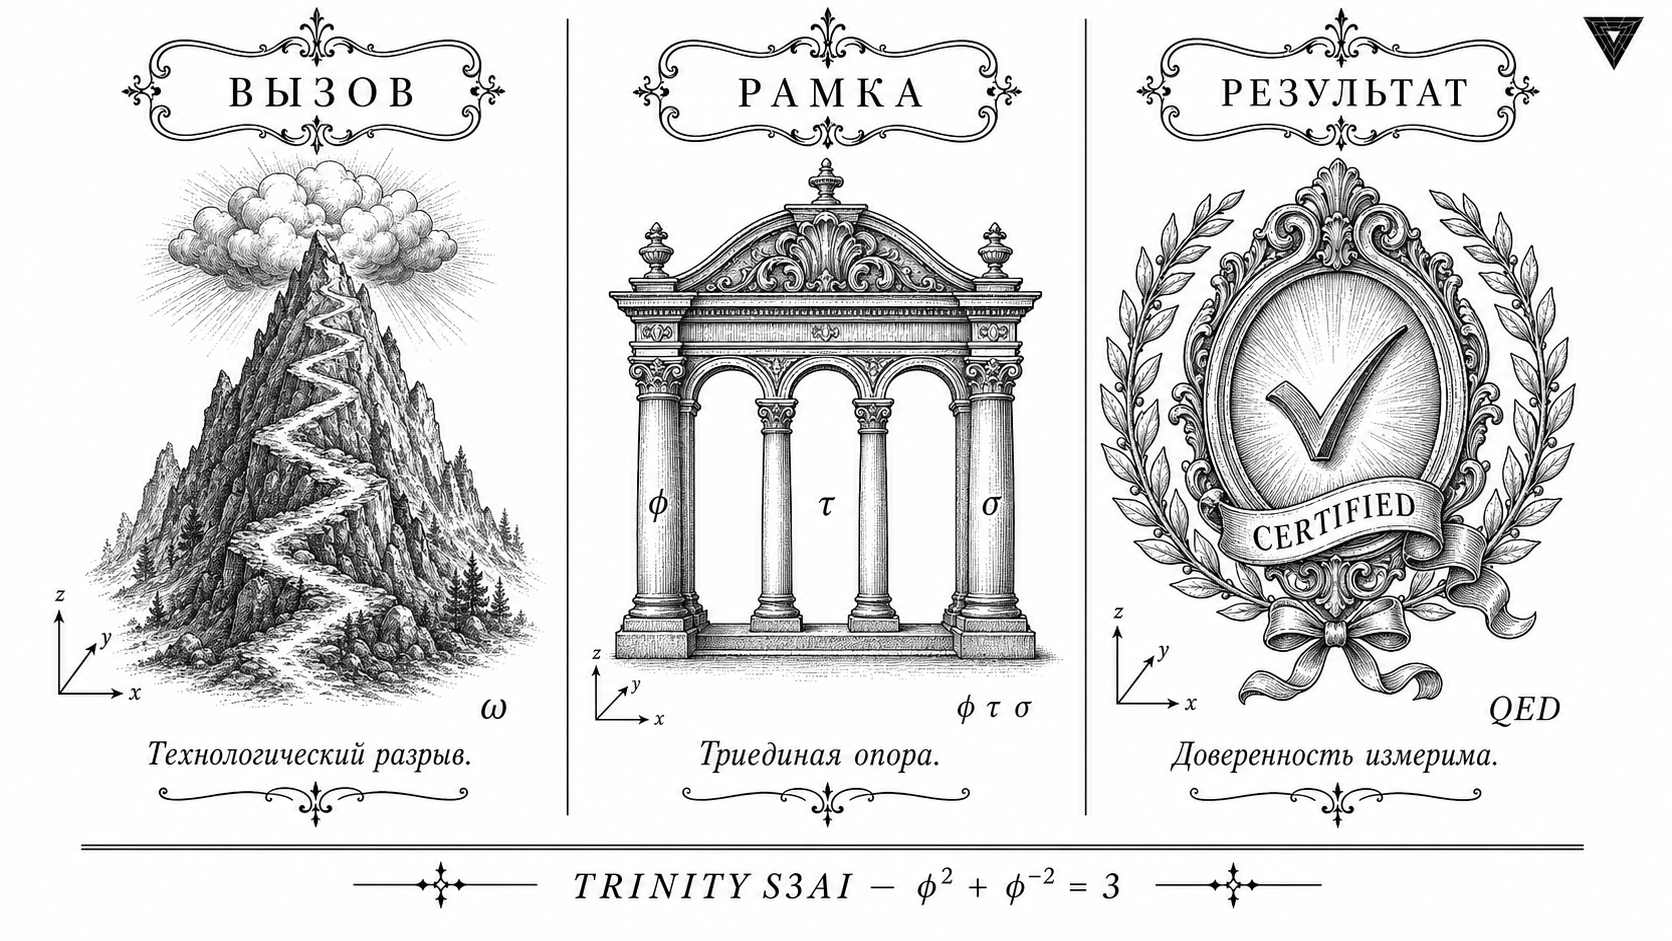
\includegraphics[keepaspectratio,alt={Аннотация --- вызов, рамка, результат}]{figures/canon/r30_annotation.png}}
\caption{Аннотация --- вызов, рамка, результат}
\end{figure}

В работе предлагается стратегическая рамка «Россия 3.0 --- Троица» ---
согласованный с действующими государственными документами подход к
достижению технологического суверенитета в сфере искусственного
интеллекта (ИИ) к 2030 году через приоритет \emph{проверяемости}
(доверенности) вычислительного стека, а не только наращивания
производительности. Показано, как ключевые целевые показатели
Национальной стратегии развития ИИ (Указ Президента РФ № 490 от
10.10.2019 в редакции Указа № 124 от 15.02.2024) и сопряжённых
документов --- нацпроекта «Экономика данных», Стратегии электронной
промышленности (Распоряжение № 20-р) и Концепции технологического
развития (Распоряжение № 1315-р) --- могут быть поддержаны открытым
отечественным заделом: семейством числовых форматов GoldenFloat,
троичной (балансной) архитектурой и спецификационно-первичным
компилятором TRI-27.

Документ строго разделяет \textbf{проверяемые факты} (опубликованный
препринт, рабочий FPGA-кодек, открытый код) и \textbf{открытые гипотезы}
(широкое принятие, энергоэффективность), помечая каждую группу
утверждений статусом. Предложение не претендует на эксклюзивность или
превосходство над государственными инициативами --- оно позиционируется
как один из готовых отечественных кирпичиков «доверенного ИИ» в смысле
действующего ГОСТ Р 59276-2020 и действующего требования Приказа ФСТЭК №
117 (п. 61); законопроект Минцифры 2026 г. привлекается лишь как вектор
регулирования {[}не действующая норма{]}. Явно выделены научная новизна
и положения, выносимые на рассмотрение; приведён протокол
воспроизводимости (открытый код, битоточные векторы, FPGA-тест-план) и
иллюстративная операционализация метрики проверяемости. Предложение
позиционировано относительно мировой литературы (posit, takum, OCP MX,
BitNet, ZKML/TEE), а также честно очерчена граница применимости тезиса:
проверяемость арифметики --- необходимая, но не достаточная часть
доверия, комплементарная проверяемости исполнения модели. Отдельно
раскрыта \textbf{ключевая отличительная особенность} стека (§ 4a):
единая программная модель --- один и тот же исходный код
(\texttt{.t27}-спецификация) сначала исполняется как «золотая» эталонная
эмуляция на обычном бинарном CPU, затем переносится на FPGA, а
результаты на обоих уровнях сверяются бит-в-бит против
единых открытых векторов соответствия; показано отличие от обычного HLS
(объединение спецификационной первичности, CPU-эталона и
SHA-256-печатей), приведён реальный кейс errata 2026-05-31 (CPU-эталон
поймал дефект до аппаратной верификации на FPGA) и трассировка
энергии (J/\text{op}) как основа «проверяемого Green AI» ---
позиционирования через достоверность энергометрики, а не гонку за
пиковыми TOPS/TOPS·Вт. Завершает работу открытое обращение к руководству
страны с семью конкретными, реализуемыми предложениями и явной встречной
отдачей государству. В версии работы дополнительно разобраны действующие
механизмы закрепления и защиты задела: патент на способ вычисления и
устройство (ст. 1350 ГК РФ), авторско-правовая охрана ИИ-кода при
доказуемом творческом вкладе человека (ст. 1257, 1259 ГК РФ), экспортный
контроль и его связь с экспортом RTL/дизайна технологии (ФЗ № 183-ФЗ; изготовление кремния за рубежом рассматривается как [замысел/будущая опция], не текущее действие),
механизм признания ПО доверенным (Постановления Правительства № 1931 и №
1912), квалификация криптофункции BLAKE3 (Постановление № 313), а также
путь стандартизации формата через ТК 164. Дополнительно приведён
конкурентный бенчмаркинг отечественного ландшафта (§ 3b: НТЦ «Модуль»,
МЦСТ, «Сбер», «Мотив НТ» «Алтай», лаб. Брусенцова, СКФУ, ИСП РАН) и
добавлена \textbf{производственная и партнёрская карта} (§ 3c: 18
отечественных фабрик-изготовителей и 9 fabless-дизайн-центров как
потенциальных партнёров по изготовлению 65--250 нм и архитектурной
кооперации, с приоритетами контакта и статусными тегами); и показана
возможность экспорта российского ядра доверия в мировую инфраструктуру
доверенных устройств «от лампочки до электронного ключа» через
действующие международные рамки (EU CRA, eIDAS 2.0, Matter, ISO/IEC
30141, FIDO2) при российском ядре (§ 8a). Отдельно предложена
операционная стратегия 2026--2030 «национальное ядро → экспорт» по
закреплению за Россией репутации доверенного поставщика ПО --- с
четырьмя годовыми этапами, измеримыми KPI и опорой на действующие нормы
РФ (Реестр ПО, «доверенное ПО», РБПО ГОСТ Р 56939) и международные
открытые стандарты прозрачности (OpenSSF Scorecard, SLSA, Sigstore,
SBOM) (§ 8b).

\textbf{Ключевые слова:} доверенный ИИ; проверяемость вычислений;
технологический суверенитет; числовые форматы (GoldenFloat); балансная
троичность; открытое железо; топология ИМС и РИД; единая программная
модель CPU→FPGA; ФСТЭК № 117; стандартизация (ТК 164).

\begin{center}\rule{0.5\linewidth}{0.5pt}\end{center}

\subsection{Суть на одной странице (для занятого
читателя)}\label{ux441ux443ux442ux44c-ux43dux430-ux43eux434ux43dux43eux439-ux441ux442ux440ux430ux43dux438ux446ux435-ux434ux43bux44f-ux437ux430ux43dux44fux442ux43eux433ux43e-ux447ux438ux442ux430ux442ux435ux43bux44f}

\begin{figure}
\centering
\pandocbounded{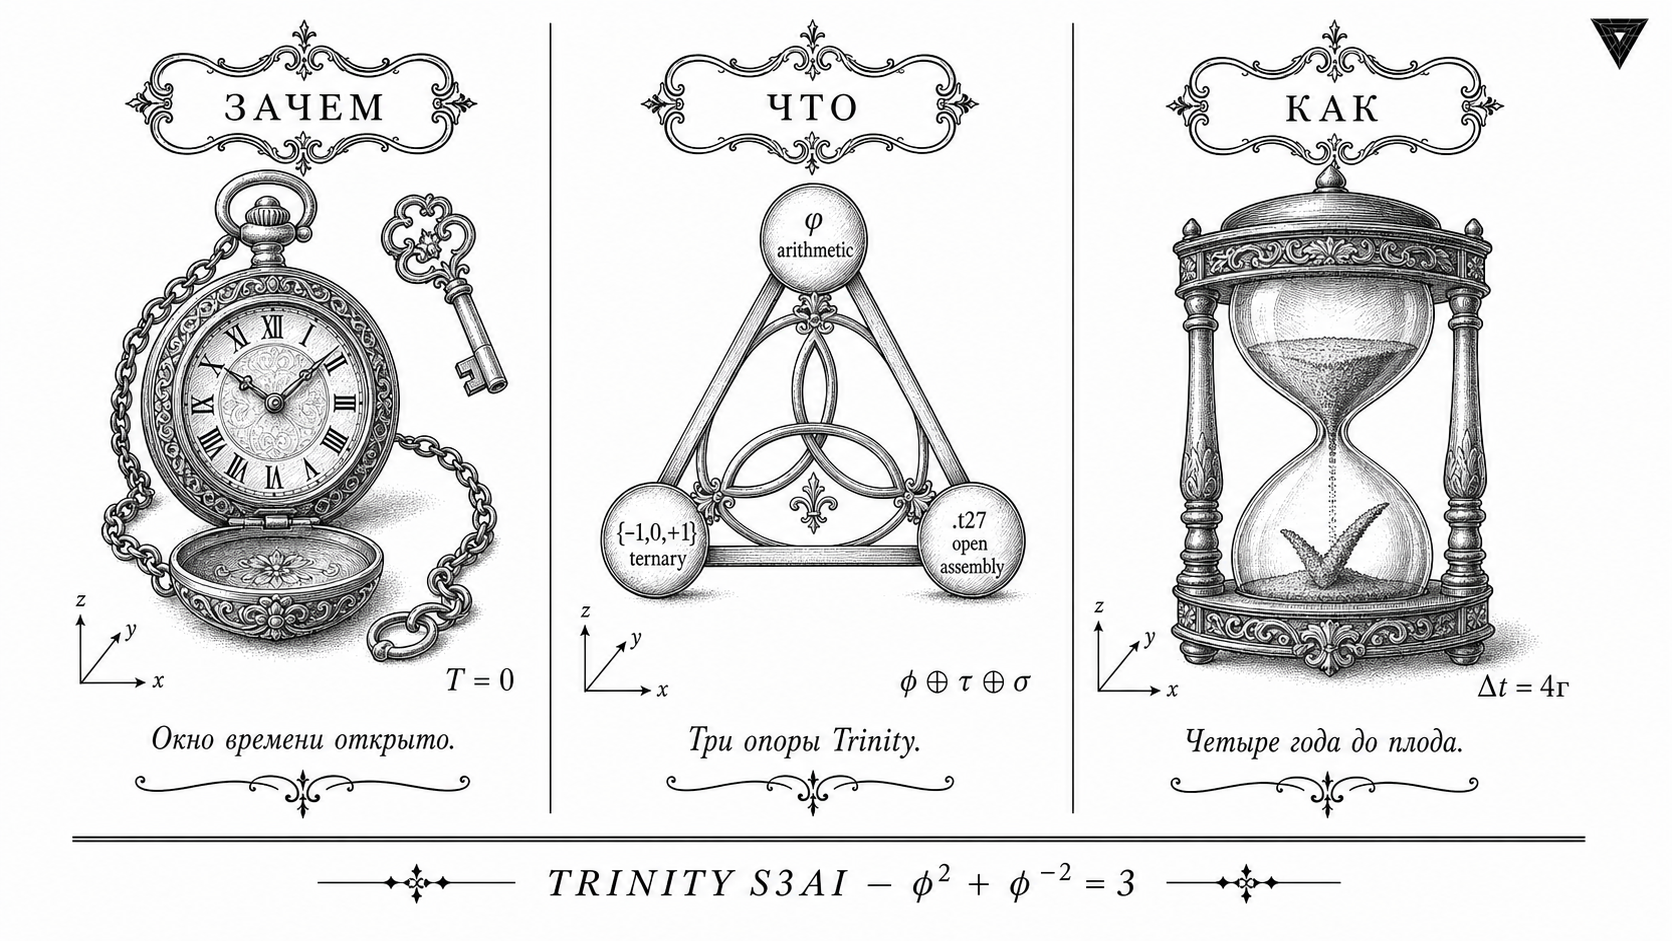
\includegraphics[keepaspectratio,alt={Суть --- зачем, что, как}]{figures/canon/r30_tldr.png}}
\caption{Суть --- зачем, что, как}
\end{figure}

\emph{Этот раздел кратко излагает всё предложение. Подробности,
источники и статусные теги --- в основном тексте.}

\textbf{Проблема.} Государство верно определило приоритетами
\textbf{доверенность и суверенитет} ИИ (Указ № 490 в ред. № 124), но у
понятия «доверенная технология» пока нет технической метрики, а гонка за
производительностью упирается в зависимость от передовой литографии.

\textbf{Идея «Россия 3.0».} Сместить приоритет первого порядка с
\emph{производительности} на \textbf{проверяемость каждого вычисления}
--- то, что можно измерить и воспроизвести на отечественной основе уже
сегодня, без потребности в 5-нм фабриках.

\textbf{Что предлагается конкретно --- стек Trinity S³AI (три опоры):}
(1) \textbf{GoldenFloat} --- числовые форматы с математически замкнутой
спецификацией; (2) \textbf{балансная троичность} \{−1, 0, +1\} ---
отечественная линия троичных машин (Сетунь); (3) \textbf{TRI-27} ---
открытый инструментарий «один код → CPU-эталон → FPGA (AX7203)» со
сверкой бит-в-бит.

\textbf{Что доказано, а что гипотеза (честно):}

\begin{itemize}
\tightlist
\item
  \textbf{{[}доказано / измерено{]}} опубликованный препринт; рабочий
  FPGA-кодек (GF16: 35/35 тестов, 323 МГц); открытый каталог 83
  форматов; открытый код под Apache-2.0/MIT.
\item
  \textbf{{[}открытая гипотеза{]}} энергоэффективность по оценке FPGA-синтеза
  (измерение на кристалле вне области работы; изготовление кремния не планируется); широкое
  принятие формата вендорами.
\end{itemize}

\textbf{О чём просьба к государству (7 мер, § 8):} включить
«проверяемость» в КПЭ доверенного ИИ; поддержать регистрацию РИД
(топология ИМС, программа для ЭВМ) для исследователей-физлиц; облегчить
вход микрокоманд в гранты; пилот доверенного инференса в рамках ЭПР;
связать публикационный и кадровый треки; ускорить стандартизацию
форматов через ТК 164; распространить патентную поддержку на
open-hardware.

\textbf{Встречная отдача государству:} неотчуждаемый отечественный РИД;
формат-кандидат в национальный стандарт (ПНСТ); учебная платформа для
кадров; проверяемый компонент доверенного ИИ под уже действующее
требование п. 61 Приказа ФСТЭК № 117. \textbf{Это инвестиция в актив, а
не безвозвратная трата.}

\begin{center}\rule{0.5\linewidth}{0.5pt}\end{center}

\subsection{1. Введение: почему «Россия 3.0» и почему
«Троица»}\label{ux432ux432ux435ux434ux435ux43dux438ux435-ux43fux43eux447ux435ux43cux443-ux440ux43eux441ux441ux438ux44f-3.0-ux438-ux43fux43eux447ux435ux43cux443-ux442ux440ux43eux438ux446ux430}

\begin{figure}
\centering
\pandocbounded{
\includegraphics[keepaspectratio,alt={Триптих фиг. 1 --- Россия 1.0 / 2.0 / 3.0: от индустриального рывка к доверенному вычислению.}]{figures/canon/r30_sec1_intro.png}}
\caption{Триптих фиг. 1 --- Россия 1.0 / 2.0 / 3.0: от индустриального
рывка к доверенному вычислению.}
\end{figure}

Россия дважды совершала технологические рывки, опираясь на собственную
научную школу. Условно их можно обозначить как \textbf{Россия 1.0} ---
индустриализация и атомно-космический проект XX века, и \textbf{Россия
2.0} --- цифровизация и построение государственных цифровых сервисов
2010--2020-х годов. Настоящая работа предлагает рамку \textbf{«Россия
3.0»} --- переход к \emph{суверенному доверенному интеллекту}, где
ценность измеряется не количеством операций в секунду, а
\textbf{проверяемостью каждого вычисления} на отечественной основе.

Название «Троица» (в английском написании --- Trinity) отсылает к
триединой опоре предлагаемого подхода: (1) \emph{доверенная арифметика}
--- числовые форматы с математически замкнутой спецификацией; (2)
\emph{доверенная логика} --- балансная троичность \{−1, 0, +1\},
продолжающая отечественную линию троичных машин; (3) \emph{доверенная
сборка} --- открытый спецификационно-первичный инструментарий, где
FPGA-битстрим воспроизводится из именованных спецификаций, а не из
непрозрачного унаследованного кода.

Выбор момента не случаен. К 1 июня 2026 года Правительству поручено
подготовить \textbf{Национальный план по внедрению технологий ИИ}
(\href{https://www.cnews.ru/news/top/2026-01-06_v_rossii_sozdayut_natsionalnyj}{перечень
поручений Президента, январь 2026 г., CNews}); 16 марта 2026 года
утверждена \textbf{дорожная карта развития суперкомпьютеров и ИИ}
(\href{https://telesputnik.ru/materials/tech/news/mixail-misustin-utverdil-doroznuyu-kartu-razvitiya-superkompyuterov-i-texnologii-ii-v-rossii}{Телеспутник});
на общественном обсуждении находится \textbf{законопроект Минцифры о
регулировании ИИ} (плановое вступление в силу --- 01.09.2027) с
введением понятий «суверенная», «национальная» и «доверенная» модель ИИ
(\href{https://pravo.ru/news/262870/}{Право.ру, март 2026}) ---
\textbf{{[}законопроект, не действующая норма{]}}. Окно для научно
обоснованных предложений открыто именно сейчас.

\begin{quote}
\textbf{Дисциплина честности (принцип данной работы).} Ниже все
утверждения о Trinity снабжены статусом: \textbf{{[}доказано{]}} ---
подтверждается публикацией или открытым кодом; \textbf{{[}измерено{]}}
--- получено на конкретном стенде; \textbf{{[}открытая гипотеза{]}} ---
заявка, путь фальсификации которой описан. Категоричные непроверяемые
утверждения («первый в мире», «лучший») не используются. Эта
самодисциплина --- не слабость, а основа доверенности в смысле ГОСТ Р
59276-2020.
\end{quote}

\begin{quote}
\textbf{Научная новизна и положения, выносимые на рассмотрение.} Чтобы
отделить новый результат от обзорной части, явно формулируем вклад
работы. \textbf{Новым является:} (1) сам \emph{критерий приоритета}
доверенного ИИ ---
\texttt{проверяемость\ на\ единицу\ стоимости\ (verifiability-per-dollar)}
--- и его операционализация через измеримые прокси (см. § 3); (2)
замкнутое правило вывода разбиения \texttt{порядок/мантисса} для
семейства форматов GoldenFloat на основе золотого сечения и его
верификация (9/9 ширин, тождество Люка до 500 знаков) (см. § 4.1); (3)
метод \emph{честного фрейминга} --- дисциплина статусных тегов
\texttt{{[}доказано{]}/{[}измерено{]}/{[}открытая\ гипотеза{]}} как
технический способ обеспечения доверия к самим заявлениям.
\textbf{Положения, выносимые на рассмотрение:} (П1) приоритет
проверяемости снимает критическую зависимость суверенного ИИ от
передовой литографии; (П2) доверенность реализуема и проверяема уже на
FPGA и доступных топологиях; (П3) задел Trinity согласован с
действующими нормами (Приказ ФСТЭК № 117 п. 61, ст. 1262 и 1448--1464 ГК
РФ) без опоры на ещё не вступивший в силу законопроект. Остальные
разделы (государственная рамка, правовой каркас) носят
обзорно-аналитический характер и служат обоснованием положений.
\end{quote}

\begin{center}\rule{0.5\linewidth}{0.5pt}\end{center}

\subsection{2. Государственная рамка: что уже зафиксировано в
документах}\label{ux433ux43eux441ux443ux434ux430ux440ux441ux442ux432ux435ux43dux43dux430ux44f-ux440ux430ux43cux43aux430-ux447ux442ux43e-ux443ux436ux435-ux437ux430ux444ux438ux43aux441ux438ux440ux43eux432ux430ux43dux43e-ux432-ux434ux43eux43aux443ux43cux435ux43dux442ux430ux445}

\begin{figure}
\centering
\pandocbounded{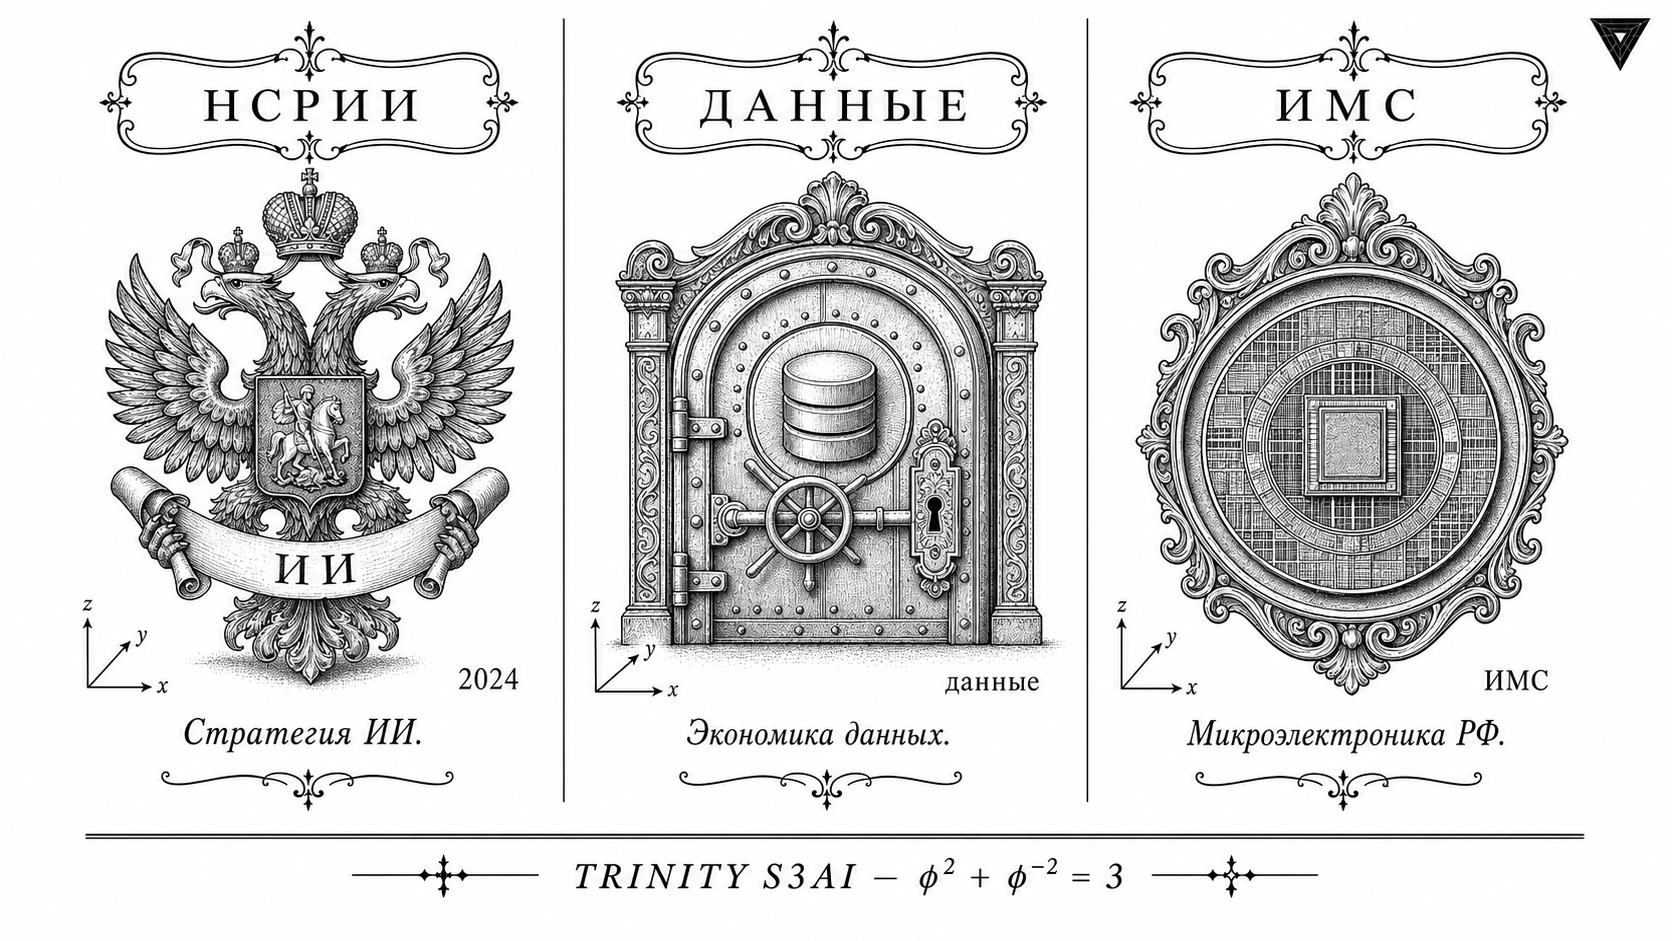
\includegraphics[keepaspectratio,alt={Триптих фиг. 2с --- Государственная рамка: НСРИИ, экономика данных, микроэлектроника.}]{figures/canon/r30_sec2_state.png}}
\caption{Триптих фиг. 2с --- Государственная рамка: НСРИИ, экономика
данных, микроэлектроника.}
\end{figure}

Предложение «Россия 3.0» не подменяет, а \emph{обслуживает} действующую
государственную политику. Ниже --- выверенные по официальным источникам
опорные документы и их целевые показатели до 2030 года.

\subsubsection{2.1. Национальная стратегия развития ИИ
(НСРИИ)}\label{ux43dux430ux446ux438ux43eux43dux430ux43bux44cux43dux430ux44f-ux441ux442ux440ux430ux442ux435ux433ux438ux44f-ux440ux430ux437ux432ux438ux442ux438ux44f-ux438ux438-ux43dux441ux440ux438ux438}

Базовый акт --- \textbf{Указ Президента РФ № 490 от 10.10.2019} «О
развитии искусственного интеллекта в Российской Федерации»
(\href{http://www.kremlin.ru/acts/bank/44731}{kremlin.ru}), действующий
в редакции \textbf{Указа № 124 от 15.02.2024}
(\href{http://www.kremlin.ru/acts/bank/50326}{kremlin.ru}). Редакция
2024 года ввела ключевые для нашего предложения понятия:
\textbf{доверенные технологии ИИ}, \textbf{прозрачность и объяснимость
алгоритмов}, \textbf{технологический суверенитет} (самостоятельность РФ
за счёт преимущественного использования отечественных технологий ИИ).

Действующие целевые показатели НСРИИ к 2030 году (верифицированы по
тексту Указа № 124):

{[}Таблица --- целевые показатели НСРИИ до 2030 г.:{]} - Затраты
организаций на внедрение ИИ: 123 млрд руб./год (2022) → \textbf{850 млрд
руб./год} (2030). - Накопленный вклад ИИ в прирост ВВП: 0,2 трлн руб. →
\textbf{11,2 трлн руб.} - Суперкомпьютерные мощности ИИ-кластеров: 0,073
→ \textbf{1 экзафлопс}; совокупные мощности сектора --- \textbf{6,2
экзафлопса}. - Выпускники вузов со специализацией ИИ: 3 048 → \textbf{15
500 чел./год}. - Доля работников с навыками ИИ: 5\% → \textbf{80\%}. -
Уровень доверия граждан к технологиям ИИ: 55\% → \textbf{80\%}. - Доля
приоритетных отраслей с высокой готовностью к внедрению ИИ: 12\% →
\textbf{95\%}. - Публикации российских авторов на конференциях ИИ уровня
A: 103 → \textbf{450 в год}.

\emph{(Источник КПЭ: \href{http://www.kremlin.ru/acts/bank/50326}{Указ №
124, kremlin.ru}.)}

Особо отметим показатель \textbf{«уровень доверия граждан к ИИ ---
80\%»}: именно его трудно достичь наращиванием производительности, и
именно к нему прямо адресован подход «проверяемости вместо TOPS».

\subsubsection{2.2. Нацпроект «Экономика данных» и федеральный проект
«Искусственный
интеллект»}\label{ux43dux430ux446ux43fux440ux43eux435ux43aux442-ux44dux43aux43eux43dux43eux43cux438ux43aux430-ux434ux430ux43dux43dux44bux445-ux438-ux444ux435ux434ux435ux440ux430ux43bux44cux43dux44bux439-ux43fux440ux43eux435ux43aux442-ux438ux441ux43aux443ux441ux441ux442ux432ux435ux43dux43dux44bux439-ux438ux43dux442ux435ux43bux43bux435ux43aux442}

С 1 января 2025 года действует национальный проект \textbf{«Экономика
данных и цифровая трансформация государства»} (2025--2030) с федеральным
бюджетом \textbf{1,013 трлн руб.}
(\href{https://www.comnews.ru/content/238087/2025-03-05/2025-w10/1007/nacproekt-ekonomika-dannykh-privlechet-14-trln-rub}{ComNews,
презентация Д. Григоренко, 26.02.2025}). В его составе --- федеральный
проект \textbf{«Искусственный интеллект»} с бюджетом \textbf{65,2 млрд
руб.} из федерального бюджета. Среди целей ФП «ИИ» --- массовое
использование \textbf{отечественных} ИИ-решений и поддержка 1 000+
ИТ-стартапов.

\subsubsection{2.3. Доверенный ИИ: действующие нормы и регуляторный
вектор}\label{ux434ux43eux432ux435ux440ux435ux43dux43dux44bux439-ux438ux438-ux434ux435ux439ux441ux442ux432ux443ux44eux449ux438ux435-ux43dux43eux440ux43cux44b-ux438-ux440ux435ux433ux443ux43bux44fux442ux43eux440ux43dux44bux439-ux432ux435ux43aux442ux43eux440}

Здесь критически важно разделить \textbf{уже действующие} требования и
\textbf{законопроект} (вектор регулирования), поскольку они имеют разную
юридическую силу.

\textbf{Действующие нормы (в силе):}

\begin{itemize}
\tightlist
\item
  \textbf{ГОСТ Р 59276-2020} «Системы искусственного интеллекта. Способы
  обеспечения доверия. Общие положения» (введён 01.03.2021,
  \href{https://docs.cntd.ru/document/1200177291}{docs.cntd.ru}) ---
  действующий стандарт, задающий понятие доверенной системы ИИ и
  классификацию способов обеспечения доверия. Развивается Техническим
  комитетом \textbf{ТК 164} «Искусственный интеллект» (серия ГОСТ:
  59277, 59898, 70462, 71476-2024, 42001-2024 и др.).
\item
  \textbf{Приказ ФСТЭК России № 117 от 11.04.2025} (в силе с 01.03.2026)
  --- новые требования к защите государственных информационных систем
  (ГИС). Пункт 61 прямо устанавливает: в состав ГИС «должны включаться
  \textbf{доверенные технологии искусственного интеллекта} или их
  компоненты»
  (\href{https://cisoclub.ru/prikaz-fstek-117/}{cisoclub.ru},
  \href{https://service.securitm.ru/docs/fstek-117/p-61}{securitm.ru}).
  Это \textbf{уже действующее} требование, формирующее реальный спрос на
  проверяемые ИИ-компоненты, а не прогноз.
\item
  \textbf{Постановление Правительства РФ № 1931 от 28.11.2025} (в силе с
  01.03.2026,
  \href{http://government.ru/docs/all/162383/}{government.ru}) ---
  механизм признания программного обеспечения \textbf{доверенным}:
  оператор --- Минцифры, процедура включает тестирование и решение
  Правительственной комиссии, статус действует 3 года. Это
  \textbf{действующая (вступающая в силу) норма}, а не законопроект, и
  она формирует отдельный, более высокий статус «доверенного ПО», к
  которому может выстраиваться трек Trinity.
\item
  \textbf{Постановление Правительства РФ № 1912 от 14.11.2023} (критерии
  доверенных программно-аппаратных комплексов, ПАК,
  \href{http://government.ru/docs/all/150563/}{government.ru}) ---
  нормативная база для доверенных ПАК на значимых объектах КИИ. Чип
  Trinity как аппаратная часть доверенного ПАК прямо вписывается в эту
  рамку.
\end{itemize}

\textbf{Регуляторный вектор (законопроект, не норма):}

\begin{itemize}
\tightlist
\item
  \textbf{Законопроект Минцифры «Об основах регулирования ИИ»}
  (опубликован 18--19 марта 2026 г., плановое вступление в силу ---
  01.09.2027,
  \href{https://amp.rbc.ru/rbcnews/technology_and_media/19/03/2026/69bb1d5a9a79470e2984c919}{РБК};
  \href{https://pravo.ru/story/263957/}{Право.ру}) --- \textbf{{[}проект
  / вектор регулирования, не действующая норма{]}}. Вводит три категории
  моделей: \textbf{суверенная} (полностью на российской базе),
  \textbf{национальная} (допускает иностранный открытый код, но на
  российских датасетах), \textbf{доверенная} (любая база, но с
  сертификатом ФСТЭК и Минцифры и внесением в реестр доверенных моделей;
  обязательна для ГИС и значимых объектов КИИ). Прямого запрета на
  иностранный ИИ законопроект не вводит. Категория «доверенная» ---
  естественная цель, к которой стек Trinity готовится заранее
  \textbf{{[}открытая гипотеза / проекция регулирования{]}}.
\end{itemize}

\subsubsection{2.4. Микроэлектроника и
техсуверенитет}\label{ux43cux438ux43aux440ux43eux44dux43bux435ux43aux442ux440ux43eux43dux438ux43aux430-ux438-ux442ux435ux445ux441ux443ux432ux435ux440ux435ux43dux438ux442ux435ux442}

\begin{figure}
\centering
\pandocbounded{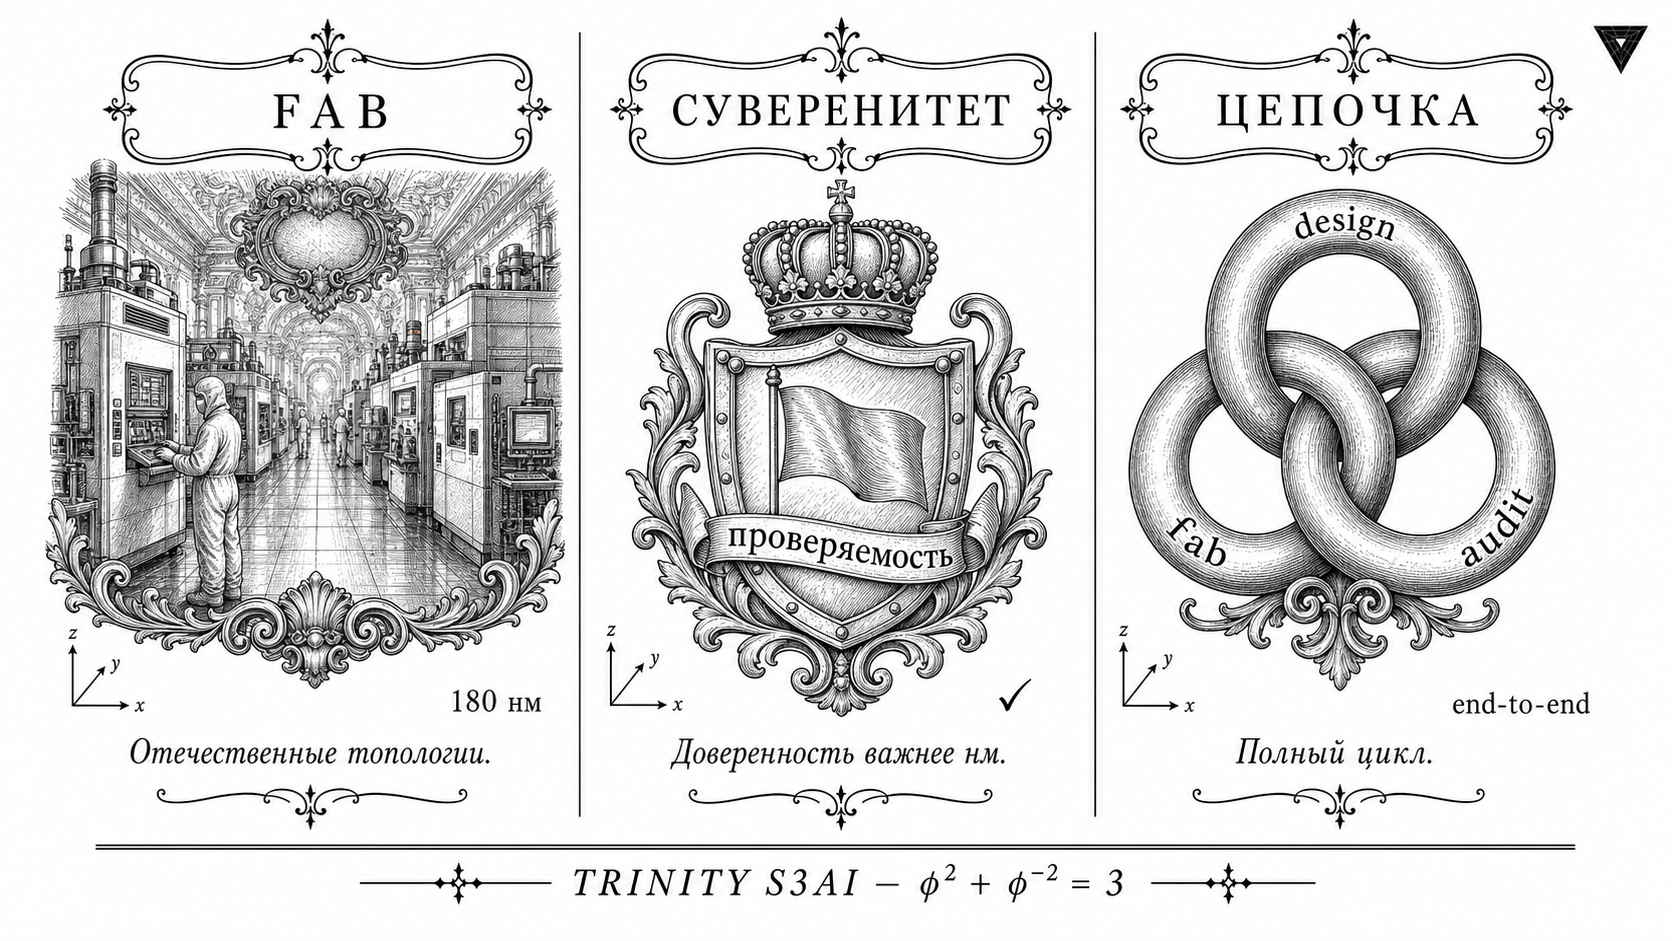
\includegraphics[keepaspectratio,alt={Микроэлектроника --- фаб, суверенитет, цепочка}]{figures/canon/r30_sec24_micro.png}}
\caption{Микроэлектроника --- фаб, суверенитет, цепочка}
\end{figure}

\textbf{Стратегия развития электронной промышленности РФ до 2030 года}
(Распоряжение Правительства № 20-р от 17.01.2020,
\href{http://government.ru/docs/38795/}{government.ru}) ставит целью
серийное производство ЭКБ по топологии \textbf{28 нм} как реалистичный
приоритет (нормы 7--5 нм --- с перспективой локализации).
\textbf{Концепция технологического развития до 2030} (Распоряжение №
1315-р от 20.05.2023) закрепляет определение технологического
суверенитета как наличия в стране собственных линий разработки
критических и сквозных технологий.

\begin{quote}
\textbf{Ключевое наблюдение.} Государственная рамка уже сместила акцент
с «догнать по нанометрам» на \textbf{«обеспечить доверенность и
суверенность»}. Подход «Россия 3.0» работает именно в этой логике:
доверенный вычислительный стек можно строить и проверять \emph{уже на
доступных топологиях и FPGA}, не дожидаясь паритета по техпроцессу.
\end{quote}

\begin{center}\rule{0.5\linewidth}{0.5pt}\end{center}

\subsection{3. Тезис «Россия 3.0»: проверяемость вместо гонки
производительности}\label{ux442ux435ux437ux438ux441-ux440ux43eux441ux441ux438ux44f-3.0-ux43fux440ux43eux432ux435ux440ux44fux435ux43cux43eux441ux442ux44c-ux432ux43cux435ux441ux442ux43e-ux433ux43eux43dux43aux438-ux43fux440ux43eux438ux437ux432ux43eux434ux438ux442ux435ux43bux44cux43dux43eux441ux442ux438}

\begin{figure}
\centering
\pandocbounded{
\includegraphics[keepaspectratio,alt={Триптих фиг. 2 --- Смена приоритета: от TOPS-per-dollar к verifiability-per-dollar.}]{figures/canon/r30_sec3_verif.png}}
\caption{Триптих фиг. 2 --- Смена приоритета: от TOPS-per-dollar к
verifiability-per-dollar.}
\end{figure}

Доминирующая мировая парадигма ИИ-инфраструктуры --- наращивание TOPS
(операций в секунду) и числа параметров моделей. В условиях ограничений
на доступ к передовой литографии прямая гонка по этому вектору для
России затруднена объективно
(\href{https://arpe.ru/news/Rossiyskoy_elektronike_ne_khvataet_innovatsiy/}{аналитика
по Стратегии № 20-р, ARPE}).

Предлагаемый сдвиг парадигмы: \textbf{измерять ценность вычислителя
проверяемостью на единицу стоимости (verifiability-per-dollar), а не
производительностью на единицу стоимости (TOPS-per-dollar)}. Это не
отказ от производительности, а смена приоритета первого порядка,
который:

\begin{enumerate}
\def\labelenumi{\arabic{enumi}.}
\tightlist
\item
  \textbf{Снимает зависимость от передовой литографии} --- доверенный
  стек верифицируется на FPGA и доступных топологиях (28 нм), что
  согласуется с реалистичным ориентиром Стратегии № 20-р.
\item
  \textbf{Прямо адресует показатель доверия граждан 80\%} ---
  объяснимая, воспроизводимая арифметика технически обосновывает
  доверие, а не декларирует его.
\item
  \textbf{Соответствует понятию доверенной системы ИИ} из действующего
  ГОСТ Р 59276-2020 (и готовит стек к категории «доверенная» будущего
  законопроекта Минцифры {[}проекция{]}) --- доверенность становится
  свойством, встроенным в стек на уровне чисел и логики, а не
  надстройкой.
\end{enumerate}

\textbf{Проверяемость измерима, а не декларативна.} Чтобы
verifiability-per-dollar был метрикой, а не лозунгом, мы
операционализируем его через конкретные технические прокси: (1)
\textbf{битоточные векторы соответствия} (bit-exact conformance vectors)
--- для каждого формата фиксированный набор эталонных значений,
воспроизводимых на любой реализации; (2) \textbf{воспроизводимость
«печатей» (seals)} компилятора TRI-27 --- детерминированная генерация
RTL из именованной \texttt{.t27}-спецификации; (3) \textbf{9/9
воспроизведение ширин порядка} реализованных форматов из единого
правила; (4) \textbf{формальная спецификация} как единый источник истины
(SSOT). Эти прокси измеримы и фальсифицируемы, что и отличает
«проверяемость» от маркетинга. \textbf{Иллюстрация операционализации
(как считать).} В первом приближении \texttt{verifiability-per-dollar}
можно оценивать как отношение
\texttt{доли\ независимо\ воспроизводимых\ результатов\ системы} (доля
выходов, прошедших битоточные векторы соответствия на независимой
реализации, 0--1) к
\texttt{совокупной\ стоимости\ владения\ вычислителем} (CAPEX+OPEX,
руб.). Для GF16-кодека сегодня доля воспроизводимых результатов = 35/35
= 1,0 на доступной FPGA стоимостью порядка десятков тысяч рублей --- то
есть высокая проверяемость достигается без передовой литографии. Это не
финальная метрика, а \textbf{пред-регистрируемый протокол измерения},
который можно уточнять и фальсифицировать \textbf{{[}смоделировано ---
методика; измерено --- числитель для GF16{]}}.

\textbf{Позиционирование (без конкуренции с ускорителями).} Trinity не
претендует на замену ИИ-ускорителей (Эльбрус, отечественные NPU,
зарубежные GPU). Это \textbf{ортогональный слой доверенной арифметики и
оракула соответствия форматам}, который может работать поверх любого
вычислителя --- отечественного или импортного --- добавляя свойство
проверяемости там, где его сегодня нет.

\textbf{Граница применимости тезиса (честно, без переоценки).}
Проверяемость \emph{арифметики и форматов} --- не то же самое, что
проверяемость \emph{модели ИИ в целом}. Галлюцинации, состязательные
атаки и ошибки обучения живут на уровне модели, \emph{выше} арифметики,
и доверенная арифметика их сама по себе не устраняет. Поэтому Trinity
решает \textbf{необходимую, но не достаточную} часть доверия:
воспроизводимый и объяснимый числовой фундамент. Он
\textbf{комплементарен}, а не альтернативен подходам проверяемости
верхнего уровня --- доказательствам с нулевым разглашением (ZKP/ZKML) и
доверенным средам исполнения (TEE), которые проверяют \emph{факт
корректного исполнения} модели
(\href{https://equilibrium.co/writing/state-of-verifiable-inference}{State
of Verifiable Inference, Equilibrium}). Полный доверенный стек
складывает оба уровня: проверяемая арифметика (Trinity) + проверяемое
исполнение (ZKP/TEE) \textbf{{[}доказано --- разграничение уровней;
открытая гипотеза --- совместная интеграция{]}}.

\textbf{Целевой ориентир для КПЭ «проверяемость» (иллюстративно).} Чтобы
предлагаемый показатель был пригоден для госплана, нужен измеримый
ориентир и метод сбора. Иллюстративно: \emph{доля доверенных
ИИ-компонентов в ГИС/КИИ, для которых публикуются битоточные векторы
соответствия и воспроизводимые сборки}, базовое значение 2026 г. ≈ 0 \%
→ целевое 2030 г. (ориентир) --- большинство критичных компонентов; сбор
--- через реестр доверенного ПО (ПП № 1931) и сертификационный трек
ФСТЭК. Конкретные пороги --- предмет согласования с регулятором
\textbf{{[}смоделировано --- методика; открытая гипотеза --- числовые
пороги{]}}.

Три опоры «Троицы» реализуют этот тезис на трёх уровнях стека.

\begin{center}\rule{0.5\linewidth}{0.5pt}\end{center}

\subsection{3a. Связанные работы и позиционирование в мировой
литературе}\label{a.-ux441ux432ux44fux437ux430ux43dux43dux44bux435-ux440ux430ux431ux43eux442ux44b-ux438-ux43fux43eux437ux438ux446ux438ux43eux43dux438ux440ux43eux432ux430ux43dux438ux435-ux432-ux43cux438ux440ux43eux432ux43eux439-ux43bux438ux442ux435ux440ux430ux442ux443ux440ux435}

\begin{figure}
\centering
\pandocbounded{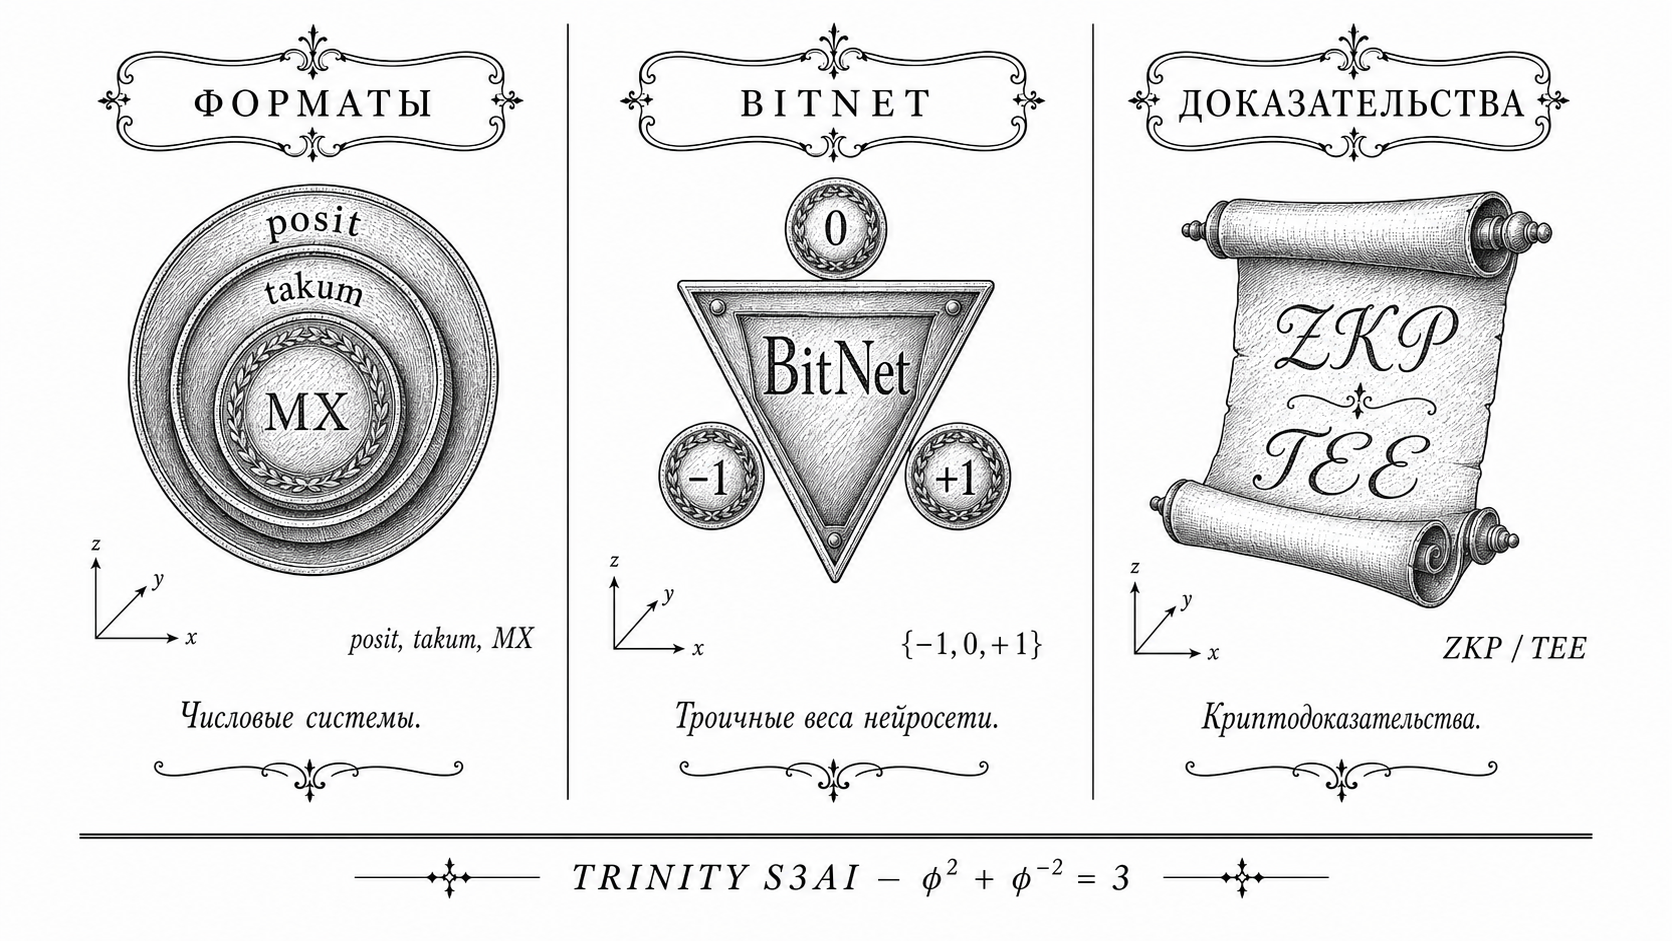
\includegraphics[keepaspectratio,alt={Триптих фиг. 3а --- Связанные работы: posit/takum/MX, BitNet \{-1,0,+1\}, ZKP/TEE.}]{figures/canon/r30_sec3a_related.png}}
\caption{Триптих фиг. 3а --- Связанные работы: posit/takum/MX, BitNet
\{-1,0,+1\}, ZKP/TEE.}
\end{figure}

Предложение Trinity опирается на три исследовательские линии и честно
соотносит себя с ними.

\textbf{Альтернативные числовые форматы.} После IEEE 754 предложен ряд
форматов: \emph{posit} (Дж. Густафсон, 2017,
\href{http://www.johngustafson.net/pdfs/BeatingFloatingPoint.pdf}{Beating
Floating Point}) с тейпер-точностью; \emph{takum} (Л. Хунхольд, 2024,
\href{https://www.arxiv.org/abs/2404.18603}{arXiv:2404.18603}) ---
логарифмический формат с ограниченным динамическим диапазоном; семейство
\emph{OCP MX / OFP8} для ML. Сравнительные оценки
(\href{http://www.arxiv.org/abs/2504.21197}{arXiv:2504.21197})
показывают преимущество тейпер-форматов над IEEE 754 по точности.
\textbf{Отличие GoldenFloat:} вклад заявляется не в точности (это
открытая гипотеза, см. § 4.1), а в \emph{замкнутом правиле вывода}
разбиения порядок/мантисса и \emph{проверяемости} (битоточные векторы,
формальная спецификация). GoldenFloat включён в нейтральный 83-форматный
каталог наряду с этими форматами.

\textbf{Троичные/малобитные вычисления.} Линия BitNet b1.58 (Microsoft)
показала, что троичные веса \{−1, 0, +1\} сохраняют качество при кратном
снижении затрат
(\href{https://github.com/huggingface/blog/blob/main/1_58_llm_extreme_quantization.md}{HuggingFace
blog}). Trinity встраивает эту линию в исторический российский контекст
«Сетуни» Брусенцова (см. § 4.2) и в доверенный стек, а не только в
эффективность.

\textbf{Проверяемые вычисления.} Параллельная линия --- ZKML и
доверенные среды (TEE) для доказательства корректного исполнения модели
(\href{https://equilibrium.co/writing/state-of-verifiable-inference}{Equilibrium}).
Как показано в § 3, Trinity работает на \emph{другом, нижнем} уровне
(арифметика/форматы) и комплементарен этим подходам. Таким образом, ниша
Trinity --- пересечение трёх линий: \emph{проверяемый числовой
фундамент} для доверенного ИИ, чего ни один из перечисленных подходов по
отдельности не закрывает.

\subsubsection{3a.1. Обновление 2026: прямые прецеденты, конкуренты и
разграничение
ниши}\label{a.1.-ux43eux431ux43dux43eux432ux43bux435ux43dux438ux435-2026-ux43fux440ux44fux43cux44bux435-ux43fux440ux435ux446ux435ux434ux435ux43dux442ux44b-ux43aux43eux43dux43aux443ux440ux435ux43dux442ux44b-ux438-ux440ux430ux437ux433ux440ux430ux43dux438ux447ux435ux43dux438ux435-ux43dux438ux448ux438}

\begin{figure}
\centering
\pandocbounded{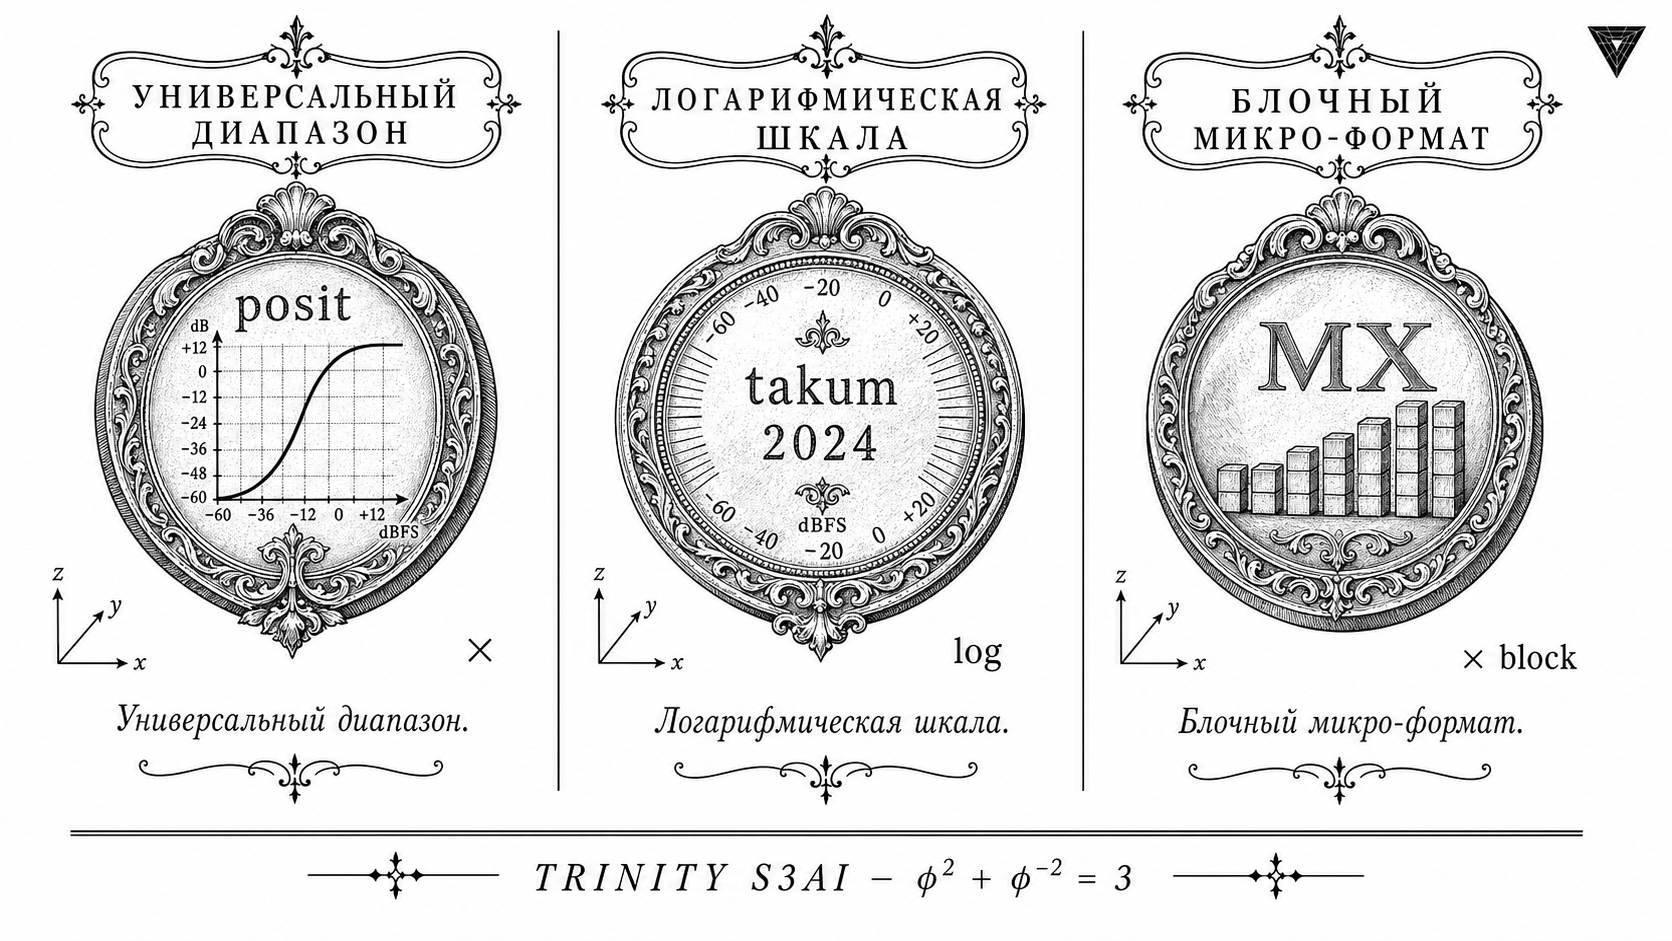
\includegraphics[keepaspectratio,alt={Прецеденты --- posit, takum, MX}]{figures/canon/r30_sec3a1_precedents.png}}
\caption{Прецеденты --- posit, takum, MX}
\end{figure}

К середине 2026 г. вокруг ниши Trinity сформировался плотный научный
фон, который требует честного разграничения. Ниже --- четыре линии с
явными статусными тегами.

\textbf{Троичные ускорители на железе (ближайшие конкуренты по нише).}
Группа FPL/FPGA опубликовала \emph{TerEffic}
(\href{https://arxiv.org/abs/2502.16473}{arXiv:2502.16473}, FPL 2025)
--- FPGA-ускоритель троично-квантованного LLM (1,58-бит веса, до 16 300
ток/с на 370M-модели) и \emph{TeLLMe}
(\href{https://arxiv.org/abs/2504.16266}{arXiv:2504.16266}, FPGA 2026)
--- первый edge-FPGA троичный ускоритель prefill+decode (7 Вт).
\textbf{Принципиальное отличие Trinity:} обе работы используют
троичность как \emph{квантизацию весов \{−1,0,+1\} поверх IEEE-FP
арифметики на FPGA}, тогда как Trinity заявляет \emph{балансную троичную
логику} \{−1,0,+1\} как RTL-дизайн, верифицируемый на FPGA AX7203. Это разные уровни: квантизация модели vs.~троичная
арифметика устройства \textbf{{[}доказано --- различие методологий{]}}.
Фундаментальный формат \emph{Tekum}
(\href{https://arxiv.org/abs/2512.10964}{arXiv:2512.10964}, Hunhold,
ноябрь 2025) вводит tapered-точность напрямую на балансной троичной
логике и является ближайшим соседом GoldenFloat по классу форматов.
\textbf{Разграничение GoldenFloat vs Tekum:} GoldenFloat использует
\emph{статическое φ-разбиение мантиссы/экспоненты} (фиксированные поля,
ориентация на ML-инференс и битоточные conformance-векторы), тогда как
Tekum --- \emph{логарифмическая tapered-кодировка} (класс takum/posit на
троичной основе, ориентация на общечисленные вычисления широкого
динамического диапазона). Tekum --- не конкурент-вытеснитель, а союзная
точка дизайн-пространства в том же классе конических/tapered форматов
\textbf{{[}доказано --- различие кодировок; возможность цитирования{]}}.

\textbf{Исторический контекст 2026.} В марте 2026 г. опубликован
\emph{5500FP} --- 24-тритный балансный троичный RISC-процессор на FPGA,
получивший освещение Hackaday и The Register. Поэтому любые формулировки
о «первом общедоступном балансном троичном железе 2026 г.» неприменимы;
Trinity дифференцируется как \emph{FPGA/RTL-дизайн для инференса ИИ с битоточно проверяемой арифметикой}, а не
general-purpose CPU на FPGA \textbf{{[}открытая гипотеза/проекция ---
позиционирование{]}}.

\textbf{Проверяемые вычисления созрели до криптографии.} Появились
\emph{NANOZK}
(\href{https://arxiv.org/abs/2603.18046}{arXiv:2603.18046}, ICLR 2026
VerifAI) --- послойные ZK-доказательства вывода LLM (доказательство 5,5
КБ, верификация 24 мс), \emph{ZK-DeepSeek}
(\href{https://arxiv.org/abs/2511.19902}{arXiv:2511.19902}) и
систематический обзор ZKML
(\href{https://arxiv.org/abs/2502.18535}{arXiv:2502.18535}).
\textbf{Позиция Trinity:} криптографические ZKP и битоточные
conformance-векторы --- \emph{разные слои гарантий}, не конкуренты. ZKP
дают математическую гарантию приватности и корректности ценой больших
ресурсов; conformance-векторы + Coq-доказательства Trinity дают
\emph{лёгкую, аппаратно реализуемую гарантию детерминизма и
воспроизводимости} нижнего арифметического уровня \textbf{{[}доказано
--- существование векторов; открытая гипотеза --- рыночное
соотношение{]}}.

\textbf{Spec-first ISA и энергетические бенчмарки.} Прямой
производственный прецедент для «спецификационно-первичного компилятора»
TRI-27 --- \emph{CHERIoT-Ibex}
(\href{https://arxiv.org/abs/2502.04738}{arXiv:2502.04738}): комплексная
формальная верификация capability-RISC-V относительно эталонной
Sail-модели (Sail→SystemVerilog→FV); инструмент \emph{Pydrofoil}
(\href{https://doi.org/10.4230/LIPIcs.ECOOP.2025.3}{ECOOP 2025}) даёт
быстрый симулятор из Sail-описания. Coq-доказательства Trinity
позиционируются как надстройка над де-факто стандартом \emph{Flocq}
(coq-flocq 4.2.1). Для воспроизводимой энергоэффективности созрели
открытые протоколы: \emph{ML.ENERGY Benchmark}
(\href{https://arxiv.org/abs/2505.06371}{arXiv:2505.06371}, NeurIPS 2025
Spotlight), \emph{Watt Counts}
(\href{https://arxiv.org/abs/2604.09048}{arXiv:2604.09048}) и
\emph{TokenPowerBench}
(\href{https://arxiv.org/abs/2512.03024}{arXiv:2512.03024}, AAAI 2026)
--- Trinity должен заявлять GF16-кодек в координатах J/op и
throughput/Watt, совместимых хотя бы с одним из них \textbf{{[}открытая
гипотеза/проекция --- численные результаты до реальных замеров{]}}.

\subsubsection{3a.2. Обновление (июнь 2026): новая волна конкурентов и
уточнение
ниши}\label{a.2.-ux43eux431ux43dux43eux432ux43bux435ux43dux438ux435-ux438ux44eux43dux44c-2026-ux43dux43eux432ux430ux44f-ux432ux43eux43bux43dux430-ux43aux43eux43dux43aux443ux440ux435ux43dux442ux43eux432-ux438-ux443ux442ux43eux447ux43dux435ux43dux438ux435-ux43dux438ux448ux438}

\begin{figure}
\centering
\pandocbounded{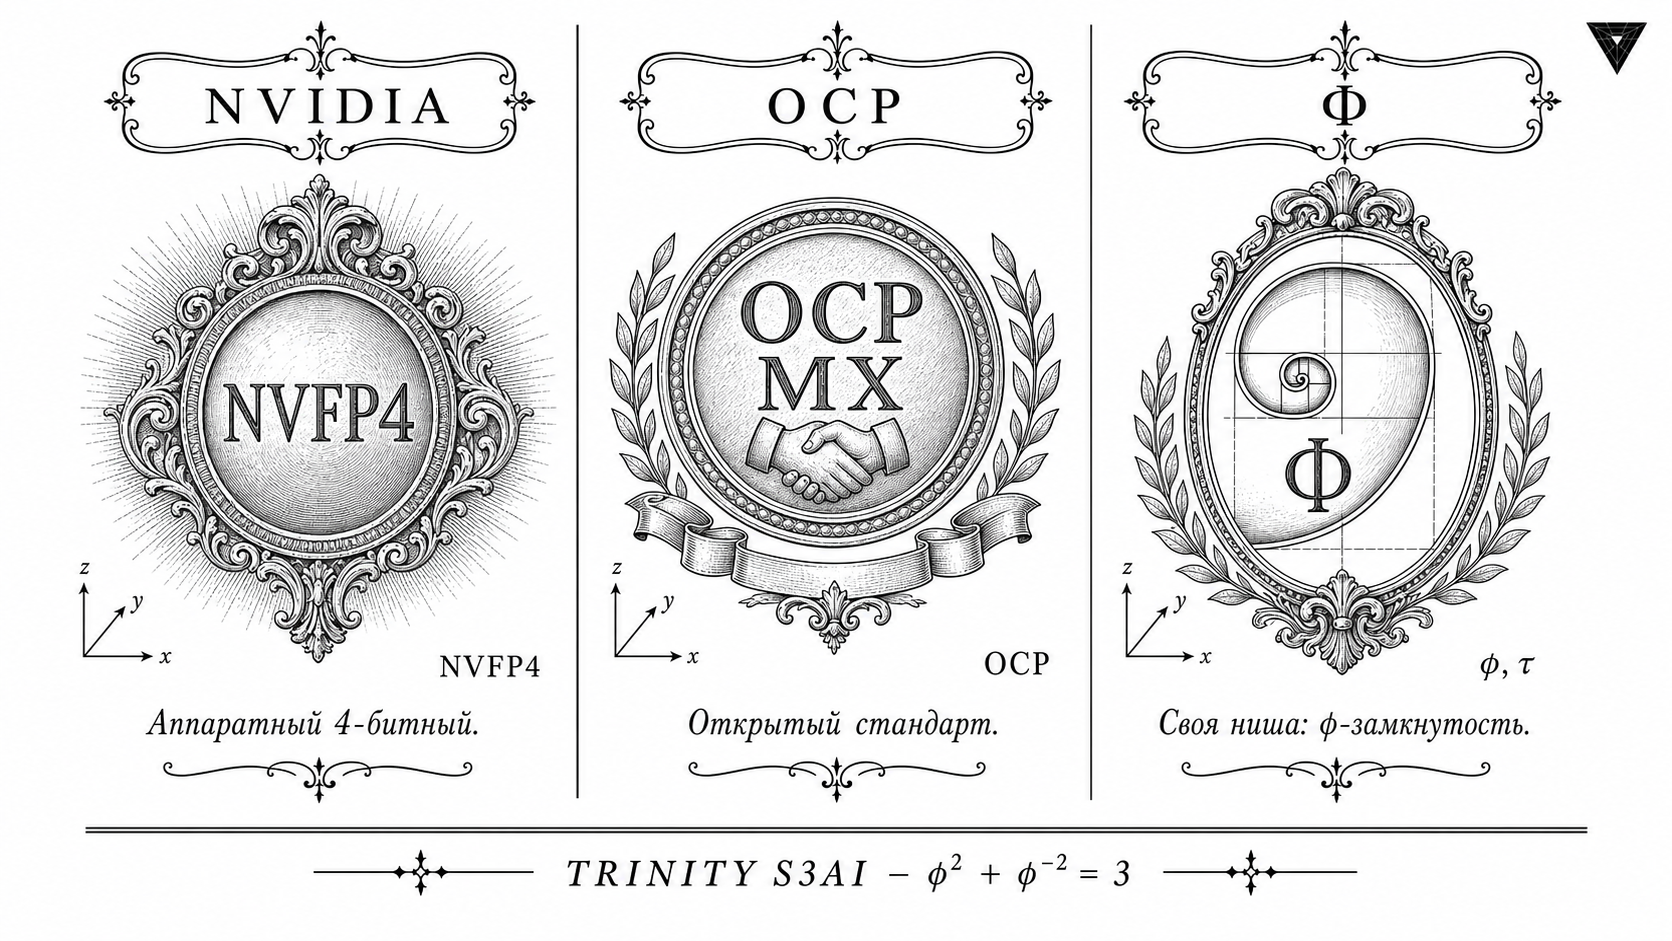
\includegraphics[keepaspectratio,alt={Волна 2026 --- NVIDIA, OCP, Φ}]{figures/canon/r30_sec3a2_wave2026.png}}
\caption{Волна 2026 --- NVIDIA, OCP, Φ}
\end{figure}

За последние месяцы конкурентный ландшафт троичных вычислений резко
уплотнился. Ниже --- честное соотнесение со свежими работами; Trinity не
претендует на превосходство по «голым» цифрам (RTL/GDS --- дизайн-артефакт, проверенный в симуляции и формально; аппаратно --- на FPGA AX7203), а
дифференцируется по трём осям: \emph{балансная троичная логика
устройства}, \emph{открытый RTL/GDS-дизайн} и
\emph{верифицируемость арифметики}.

\textbf{Троичные ускорители ASIC/CPU --- планка поднялась.} \emph{TENET}
от Microsoft Research
(\href{https://arxiv.org/abs/2509.13765}{arXiv:2509.13765}) ---
sparse-aware LUT-центричная архитектура троичного LLM-инференса:
TENET-ASIC заявляет 21,1× энергоэффективности и 2,7× ускорения против
A100 \textbf{{[}доказано --- у авторов{]}}. \emph{TOM}
(\href{https://arxiv.org/abs/2602.20662}{arXiv:2602.20662}) синтезирует
троичные веса как standard-cell ROM (3 306 ток/с на BitNet-2B).
\emph{T-SAR} (\href{https://arxiv.org/abs/2511.13676}{arXiv:2511.13676},
DATE 2026) и \emph{Litespark}
(\href{https://arxiv.org/abs/2605.06485}{arXiv:2605.06485}) показывают
троичный инференс \textbf{на обычном CPU без спец-железа} (до 52×
throughput через SIMD). \textbf{Разграничение Trinity:} все они
используют троичность как \emph{квантизацию весов \{−1,0,+1\} поверх
бинарной арифметики} (LUT-декомпрессия, ROM, SIMD-эмуляция); Trinity
заявляет \emph{балансную троичную логику как RTL-дизайн} с
битоточно верифицируемой арифметикой на FPGA AX7203. Software-троичность на бинарном
CPU и native-троичный RTL-дизайн на FPGA --- не взаимоисключающие: GF16/TRI-27
остаётся переносимым числовым форматом и эталоном \textbf{{[}доказано
--- различие методологий; открытая гипотеза --- энергетическое сравнение
до измерения на FPGA{]}}. \emph{TeLLMe} перешёл из препринта в
рецензируемую публикацию ACM FPGA 2026
(\href{https://doi.org/10.1145/3748173.3779191}{DOI
10.1145/3748173.3779191}), что усиливает его вес как прецедента.

\textbf{ZKML без спец-железа.} \emph{Jolt Atlas}
(\href{https://arxiv.org/abs/2602.17452}{arXiv:2602.17452}) расширяет
ZK-доказательства напрямую на ONNX-операции со streaming-доказательством
на устройствах с ограниченной памятью --- то есть ZK-инференс без ASIC.
\textbf{Позиция Trinity остаётся в силе:} битоточные conformance-векторы
+ Coq/Flocq дают \emph{детерминированную воспроизводимость нижнего
арифметического уровня} (лёгкую, аппаратно реализуемую), тогда как ZKP
(Jolt Atlas, NANOZK) дают \emph{криптографическую приватность и
корректность исполнения}. Это разные слои гарантий, которые можно
складывать, а не конкуренты \textbf{{[}доказано --- существование
conformance-векторов; открытая гипотеза --- рыночное соотношение{]}}.

\textbf{Канонический якорь энергометрики и зрелость Sail.} Позиционная
работа \emph{«LLM Inference as Energy-to-Token Production»}
(\href{https://arxiv.org/abs/2605.11733}{arXiv:2605.11733}, май 2026)
формализует именно те метрики (J/token, PUE-adjusted power, Token
Production Function), в которых Trinity заявляет energy-harness GF16 ---
это даёт прямую привязку к актуальному академическому дискурсу
\textbf{{[}возможность цитирования{]}}. Экосистема \emph{Sail} за
апрель--май 2026 укрепилась как мейнстрим spec-first ISA: формализация
RISC-V Hypervisor Extension в Sail (ASPLOS 2026,
\href{https://doi.org/10.1145/3803525.3804982}{DOI
10.1145/3803525.3804982}), Interaction-Tree-семантика RISC-V в Rocq и
фреймворк \emph{ArchSem} (Proceedings of the ACM on Programming
Languages, POPL 2026, vol.10, \href{https://doi.org/10.1145/3776650}{DOI
10.1145/3776650}) от кембриджской Sail-группы. Это подтверждает:
Sail-описание TRI-27 ISA --- корректно позиционированный вклад, а не
экзотика \textbf{{[}подтверждает позиционирование{]}}. Параллельно
усиливается линия posit-на-RISC-V (\emph{QVU}, IEEE ISPA 2025,
\href{https://doi.org/10.1109/ISPA67752.2025.00020}{DOI
10.1109/ISPA67752.2025.00020}; унифицированный posit/IEEE-754-кодек,
\href{https://arxiv.org/abs/2505.19096}{arXiv:2505.19096}) --- прямое
конкурентное давление на нишу «новый числовой формат как
ISA-расширение»; ответ Trinity --- позиционировать GoldenFloat как
отдельную точку дизайн-пространства с замкнутой спецификацией и ускорять
стандартизацию формата через ТК 164 \textbf{{[}открытая
гипотеза/проекция{]}}.

\begin{center}\rule{0.5\linewidth}{0.5pt}\end{center}

\subsubsection{3a.3. Обновление (июль 2026): ASIC-планка Platinum,
метрика AUE и зрелость
Lean/Rocq-верификации}\label{a.3.-ux43eux431ux43dux43eux432ux43bux435ux43dux438ux435-ux438ux44eux43bux44c-2026-asic-ux43fux43bux430ux43dux43aux430-platinum-ux43cux435ux442ux440ux438ux43aux430-aue-ux438-ux437ux440ux435ux43bux43eux441ux442ux44c-leanrocq-ux432ux435ux440ux438ux444ux438ux43aux430ux446ux438ux438}

К июлю 2026 г. фон уплотнился ещё по трём осям. Ниже --- честное
соотнесение с источниками, не цитированными выше; статусные теги
сохранены, превосходство по «голым» цифрам не заявляется (RTL/GDS
— дизайн-артефакт: проверен в sim и формально; аппаратно — на FPGA AX7203).

\textbf{ASIC-планка поднялась снова --- Platinum как новая базовая
линия.} На ASP-DAC 2026 принят \emph{Platinum}
(\href{https://arxiv.org/abs/2511.21910}{arXiv:2511.21910},
\href{https://doi.org/10.1109/ASP-DAC66049.2026.11420289}{DOI
10.1109/ASP-DAC66049.2026.11420289}, Duke University) --- лёгкий
LUT-ориентированный ASIC-ускоритель mpGEMM с офлайн-генерируемыми путями
и адаптивным переключением между bit-serial и троичным режимами; на
BitNet b1.58-3B авторы заявляют 73,6× ускорения и 32,4× снижения
энергопотребления против SpikingEyeriss при площади 0,96 мм²
\textbf{{[}доказано --- у авторов{]}}. \emph{PD-Swap}
(\href{https://arxiv.org/abs/2512.11550}{arXiv:2512.11550}) добавляет
давление в FPGA-сегменте: дезагрегированный prefill/decode-ускоритель
ternary-LLM на динамической частичной реконфигурации (27 ток/с, 1,3-2,1×
против SOTA на длинных контекстах). \textbf{Разграничение Trinity без
изменений и теперь с явным ASIC-репером:} все три (Platinum, PD-Swap,
ранее TeLLMe/TENET) используют троичность как \emph{квантизацию весов
\{−1,0,+1\} поверх бинарной арифметики}; Trinity заявляет
\emph{балансную троичную логику как RTL-дизайн, верифицируемый на FPGA AX7203} с битоточно
верифицируемой арифметикой. Это разные уровни, а не сравнение «кто
быстрее»; численное энергетическое сопоставление с Platinum остаётся
\textbf{{[}открытой гипотезой/проекцией до измерения на FPGA{]}}.

\textbf{Метрика энергоэффективности уточнилась --- AUE поверх J/token.}
Работа \emph{AUE}
(\href{https://doi.org/10.1109/ICPADS67057.2025.11323149}{DOI
10.1109/ICPADS67057.2025.11323149}, ICPADS 2025) показывает, что сырой
J/token систематически искажает сравнение в пользу малых моделей, и
предлагает нормированную метрику AUE = Дж / (KToken × GParam),
нейтральную к масштабу модели. Это прямо релевантно линии § 4a.3:
энергетические сравнения GF16-кодека Trinity с float-базовыми линиями
следует приводить \textbf{в координатах AUE}, а не только J/token, чтобы
сопоставление было честным относительно размера модели
\textbf{{[}возможность цитирования{]}}. Эмпирическая работа группы
Luccioni (\href{https://arxiv.org/abs/2601.22362}{arXiv:2601.22362},
январь 2026, NVIDIA H100) уточняет границу применимости: квантизация
даёт реальную экономию энергии \emph{только в compute-bound режиме}, а
на системном уровне scheduling запросов может менять энергию на запрос
до 100× \textbf{{[}подтверждает позицию{]}}. Вывод для Trinity: троичная
арифметика выигрывает именно в compute-bound режиме --- это совпадает с
режимом, где квантизация реально снижает энергию; следовательно, заявку
об энергоэффективности нужно формулировать как условную («в
compute-bound нагрузке»), а не безусловную, и измерять в AUE.

\textbf{Верификация арифметики и ISA --- производственная зрелость
Lean/Rocq.} Появились прямые инструментальные прецеденты для линии § 4a
(Coq/Flocq-надстройка Trinity): \emph{LeanBET}
(\href{https://arxiv.org/abs/2605.16169}{arXiv:2605.16169}, май 2026)
--- исполняемый научный конвейер в Lean 4, который ведёт
float-вычисление и одновременно доказывает корректность над
вещественными числами, то есть демонстрирует ту же дуальную стратегию
«исполнение + вещественное доказательство», что заявляет Trinity
\textbf{{[}подтверждает позицию{]}}; \emph{NumFuzz}
(\href{https://arxiv.org/abs/2501.14598}{arXiv:2501.14598}, PACMPL) и
\emph{VCFloat2} (\href{https://doi.org/10.1145/3636501.3636953}{DOI
10.1145/3636501.3636953}, CPP 2024) дают тип-системные и Coq-инструменты
автоматического вывода границ ошибок округления для \emph{нестандартных}
форматов (настраиваемая ширина мантиссы) --- прямой прецедент для
верификации форматов каталога Trinity \textbf{{[}возможность
цитирования{]}}. Линию spec-first ISA расширяет
\emph{Interaction-Tree-семантика RISC-V на Rocq}
(\href{https://arxiv.org/abs/2605.04933}{arXiv:2605.04933}, май 2026):
сквозная bisimulation «LLVM IR → RTL» с case study корректности ALU ---
тот тип кросс-уровневой верификации, который Trinity позиционирует для
TRI-27 \textbf{{[}подтверждает позиционирование{]}}.

\textbf{ZKML --- окно ниши продолжает сужаться.} \emph{TeleSparse}
(\href{https://arxiv.org/abs/2504.19274}{arXiv:2504.19274}) снизил
память доказателя ZK-верификации трансформеров на 67 \% и время на 46 \%
(Halo2, проверено на ViT/ResNet/MobileNet) при потере точности
\textasciitilde1 \% --- то есть ZK-верификация инференса становится
практичной без спецжелеза. \textbf{Позиция Trinity остаётся прежней и
проверяемой:} битоточные conformance-векторы + Coq/Flocq дают
\emph{детерминированную воспроизводимость нижнего арифметического
уровня} (лёгкую, аппаратно реализуемую), ZKP (TeleSparse, ранее
ZK-DeepSeek/Jolt Atlas/NANOZK) дают \emph{криптографическую приватность
и корректность исполнения} --- это складываемые слои, а не конкуренты
\textbf{{[}доказано --- существование conformance-векторов; открытая
гипотеза --- рыночное соотношение{]}}.

\subsubsection{3a.4. Обновление (июль 2026, вторая половина):
Lean-формализация P3109, единая DSE-рамка для троичных ускорителей и
давление posit/takum на
RISC-V}\label{a.4.-ux43eux431ux43dux43eux432ux43bux435ux43dux438ux435-ux438ux44eux43bux44c-2026-ux432ux442ux43eux440ux430ux44f-ux43fux43eux43bux43eux432ux438ux43dux430-lean-ux444ux43eux440ux43cux430ux43bux438ux437ux430ux446ux438ux44f-p3109-ux435ux434ux438ux43dux430ux44f-dse-ux440ux430ux43cux43aux430-ux434ux43bux44f-ux442ux440ux43eux438ux447ux43dux44bux445-ux443ux441ux43aux43eux440ux438ux442ux435ux43bux435ux439-ux438-ux434ux430ux432ux43bux435ux43dux438ux435-posittakum-ux43dux430-risc-v}

К середине июля 2026 г. фон уплотнился по четырём осям, ранее не
отражённым в § 3a.1--3a.3. Разграничение ниши сохраняется; статусные
теги приводятся; численное превосходство не заявляется (RTL/GDS
— дизайн-артефакт: проверен в sim и формально; аппаратно — на FPGA AX7203).

\textbf{Формальная верификация узкобитной арифметики: у конкурирующего
формат-класса появился machine-checked фундамент.} Работа \emph{FLoPS}
(\href{https://arxiv.org/abs/2602.15965}{arXiv:2602.15965}, v3 май 2026,
Rutgers) даёт, по заявлению авторов, первую машинно-проверенную
Lean-формализацию грядущего стандарта \emph{IEEE-P3109} для малоточной
floating-point арифметики --- параметрического семейства форматов
(произвольная ширина, точность вплоть до 1-битной мантиссы, stochastic
rounding, saturation); в ней доказано новое свойство точного
overflow-error у FastTwoSum при saturation и показан слом свойств
ExtractScalar при 1 бите точности. \textbf{Соотнесение с Trinity:} это
одновременно {[}возможность цитирования{]} --- прямой прецедент
формализации целого стандарта форматов, на который опирается наш
собственный verification-нарратив (Coq/Flocq над каталогом GoldenFloat),
--- и {[}конкурент/угроза{]}, поскольку P3109 как класс узкобитных FP
теперь получает независимый машинно-проверенный базис. Позиционирование
GoldenFloat корректно формулировать не как «более верифицируемый
формат», а как \emph{другой класс} (φ-производный статический split
против параметрического P3109) с \emph{собственным} уровнем аудита ---
битоточными conformance-векторами и FPGA-кодеком, измеренным на Tier-E
\textbf{{[}verified SW; измерено CI-synth/FPGA --- для отдельных
ступеней GF{]}}.

\textbf{Троичные ускорители получают единую систему сравнения
(DSE-рамку).} Группа KU Leuven
(\href{https://arxiv.org/abs/2604.25183}{arXiv:2604.25183}, апрель 2026)
формализует пространство проектирования LUT-based троичных ускорителей
класса BitNet b1.58, публикует открытый генератор + аналитическую модель
стоимости, верифицированную синтезом TSMC 16 нм, и заявляет экономию
площади до 2,2× против multiplier-baseline с коррекцией параметров ряда
SOTA-дизайнов до 1,2×. \textbf{Значение для Trinity:} это
{[}конкурент/угроза{]} на уровне \emph{методологии} --- любые будущие
сравнения троичного железа Trinity с классом BitNet-ускорителей (TENET,
TeLLMe, VitaLLM) будут, вероятно, оцениваться сквозь эту DSE-рамку.
Разграничение при этом не меняется: перечисленные работы трактуют
троичность как \emph{квантизацию весов \{−1,0,+1\} поверх бинарной
арифметики}, тогда как Trinity заявляет \emph{балансную троичную логику
как RTL-дизайн, верифицируемый на FPGA} с битоточно проверяемой арифметикой. Разумный
тактический вывод --- привести собственные FPGA-метрики GoldenFloat (LUT
decode-кодека, Tier-E) в терминах, сопоставимых с осями стоимости этой
рамки, а не отвечать на неё «голыми» TOPS \textbf{{[}возможность
цитирования --- как источник инженерных ограничений LUT-ядер{]}}.

\textbf{Posit/takum и spec-first ISA продолжают наращивать инженерное
давление.} Линия альтернативных числовых форматов на открытой
RISC-V-интеграции --- прямое референсное поле GoldenFloat ---
уплотнилась: precision-scalable posit/IEEE-754-кодеки в ядре RISC-V
(\href{https://arxiv.org/abs/2505.19096}{arXiv:2505.19096}) заявляют
сокращение LUT на 47,9 \% и FF на 57,4 \% с ускорением GEMM до 2,54×
относительно прежних posit-RISC-V реализаций; сравнительная эмпирика
takum vs posit vs OFP8/bfloat16 продолжает накапливаться в пользу
takum16 как «жизнеспособного кандидата» на замену bfloat16 (по заявлению
авторов соответствующих работ). На стороне формальной ISA-модели
\emph{Modular SAIL}
(\href{https://arxiv.org/abs/2507.12471}{arXiv:2507.12471})
демонстрирует композициональность golden-модели SAIL-RISCV на уровне
эмулятора с сохранением функциональной эквивалентности монолиту.
\textbf{Соотнесение:} takum остаётся \emph{союзником по классу}
(конические/tapered форматы), а не «врагом»; posit-RISC-V и Modular SAIL
--- {[}конкурент/угроза{]} и одновременно {[}возможность цитирования{]}
как прецеденты модульных, проверяемых форматных ISA-расширений, на
которые может опереться собственный трек ПНСТ GoldenFloat через
профильный ТК.

\textbf{Энергетическая метрика: от J/token к методологически оговорённым
осям.} В дополнение к AUE (§ 3a.3) работа \emph{Advocating
Energy-per-Token}
(\href{https://arxiv.org/abs/2603.20224}{arXiv:2603.20224}) предлагает
energy-per-token как метрику-дополнение к accuracy-бенчмаркам и
показывает, что chain-of-thought способен увеличивать энергозатраты
малых моделей в 130--150× (величина разрыва --- по методологии авторов,
требует независимой проверки). \textbf{Вывод для Trinity без изменений и
теперь с двумя опорами:} заявку об энергоэффективности GF16-кодека
формулировать \emph{условно} (compute-bound режим) и приводить
одновременно в координатах AUE и energy-per-token, а не как безусловное
«49×» --- последнее сохраняет статус \textbf{{[}открытой
гипотезы/проекции до измерения на FPGA{]}}.

\begin{center}\rule{0.5\linewidth}{0.5pt}\end{center}

\subsection{3b. Отечественный ландшафт и конкурентный
бенчмаркинг}\label{b.-ux43eux442ux435ux447ux435ux441ux442ux432ux435ux43dux43dux44bux439-ux43bux430ux43dux434ux448ux430ux444ux442-ux438-ux43aux43eux43dux43aux443ux440ux435ux43dux442ux43dux44bux439-ux431ux435ux43dux447ux43cux430ux440ux43aux438ux43dux433}

\begin{figure}
\centering
\pandocbounded{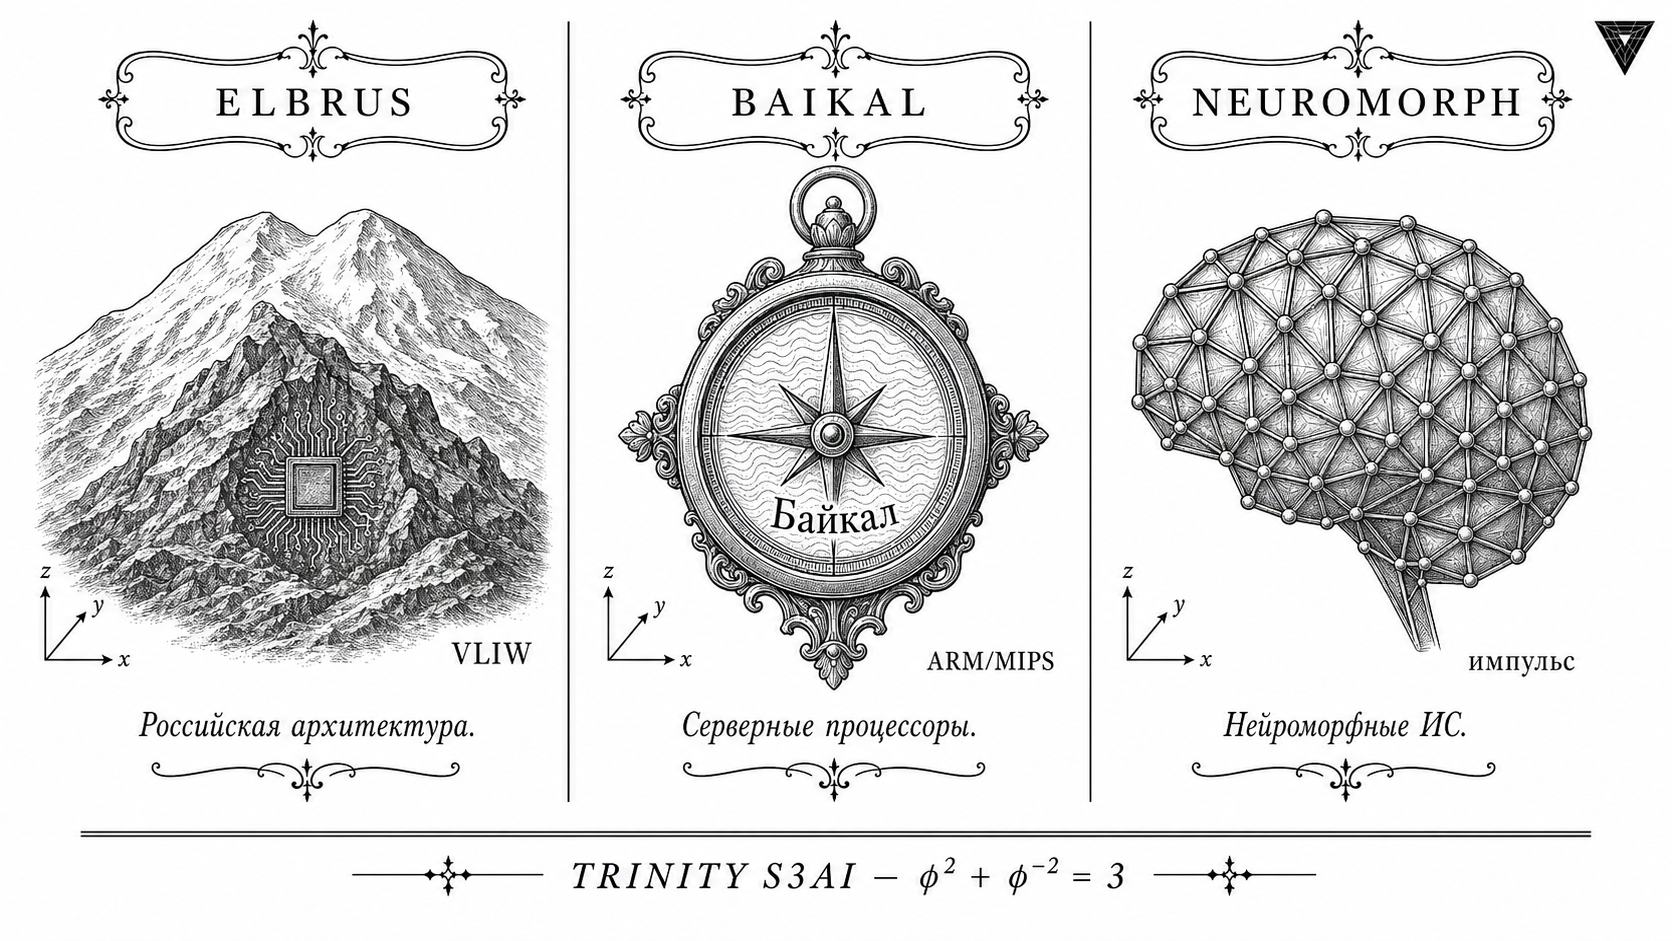
\includegraphics[keepaspectratio,alt={Триптих фиг. 3б --- Отечественный ландшафт: Эльбрус, Байкал, нейроморфные ИС.}]{figures/canon/r30_sec3b_landscape.png}}
\caption{Триптих фиг. 3б --- Отечественный ландшафт: Эльбрус, Байкал,
нейроморфные ИС.}
\end{figure}

Чтобы позиционирование «проверяемость вместо TOPS» не звучало
абстрактно, ниже честно соотнесём Trinity с \textbf{реальными
отечественными игроками}. Российский ландшафт релевантных технологий
распадается на четыре слоя; Trinity заявлена во всех четырёх, но с
\emph{разной зрелостью} --- сильнее в L3 (форматы, опубликованы) и L4
(правовой и верификационный каркас), слабее в L1/L2 (RTL/GDS — дизайн-артефакт,
аппаратная верификация — на FPGA AX7203; изготовление кремния не планируется). Все характеристики
конкурентов взяты из открытых источников на середину июня 2026 г. и
снабжены статусными тегами; заявления вендоров атрибутируются источнику,
а не нам.

\textbf{L1 --- ИИ-ускорители и нейропроцессоры.} Старейший и наиболее
зрелый разработчик --- \textbf{НТЦ «Модуль»} (архитектура NeuroMatrix):
флагман К1879ВМ8Я/NM6408 (28 нм, 16 ядер NMC4 @1 ГГц, \textasciitilde512
GFLOPS fp32, 20--35 Вт, серийно с 2019 г.) \textbf{{[}измерено{]}}
(\href{https://habr.com/ru/articles/922958/}{разбор NM Card, Habr});
перспективная линейка на NMC5 --- «Арамис» (64 TOPS@int8, 12 Вт) и
«Портос» (16 TFLOPS@fp64, 150 Вт), первый продукт ожидается в 2027 г.
\textbf{{[}смоделировано{]}}
(\href{https://tehnoomsk.ru/archives/18434}{Техносфера}). \textbf{МЦСТ
«Эльбрус»} --- универсальные процессоры (Эльбрус-2С3 партией
\textgreater10 тыс. шт. за 2025 г.; Эльбрус-32С, 7 нм, ≥6 TFLOPS,
предсерия не ранее 2027 г.) \textbf{{[}доказано/смоделировано{]}}
(\href{https://zhukovsky.life/news/12711/}{Жуковский Life}); отдельный
«Эльбрус-Б» Бабаянов обещает «в 30--200 раз», но прототип не показан
\textbf{{[}открытая гипотеза{]}}
(\href{https://importfree.cnews.ru/news/top/2025-05-12_osnovatel_mtsst_i_vyhodets}{CNews}).
\textbf{«Сбер»} на ПМЭФ-2026 показал фотонный вычислитель (\textgreater1
млрд матричных умножений/с, энергопотребление оптического ядра «более
чем на 30\% ниже электронных аналогов») \textbf{{[}смоделировано{]}}
(\href{https://www.gazeta.ru/amp/business/news/2026/06/04/28617565.shtml}{Газета.Ru}).
\textbf{НПЦ «Элвис»} разрабатывает доверенный сетевой процессор
«МАРКО-240» (ОКР Минпромторга) \textbf{{[}доказано{]}}
(\href{https://vpk.name/news/474097_minpromtorg_razdal_20_mlrd_na_novye_rossiiskie_processory.html}{ВПК.name})
--- релевантен мере по доверенным сетям, но это сетевой процессор, а не
ИИ-арифметика.

\textbf{L2 --- нейроморфные процессоры.} Наиболее близкий по духу
конкурент по \emph{энергоэффективности} --- \textbf{«Мотив НТ» «Алтай»
(AltAI)}: цифровой импульсный (SNN) процессор, 28 нм, 16 нейроядер, до
8192 нейронов, \textasciitilde4 млн синапсов, энергопотребление
\textbf{70--300 мВт}, вычисления-в-памяти \textbf{{[}измерено{]}}
(прототип AltAI-1)
(\href{https://memrilab.polyketon.ru/ru/blog/altai/}{MemriLAB},
\href{https://neuro.kaspersky.ru/processor-altai/}{Kaspersky
Neuromorphic}); заявление «примерно в 1000 раз меньше энергии, чем GPU»
--- \textbf{{[}смоделировано / заявление вендора{]}}, не независимый
замер. \textbf{Курчатовский институт и ННГУ} ведут мемристорные
нейроядра на уровне прототипов \textbf{{[}доказано{]}}
(\href{https://hightech.fm/2024/12/24/memristor-neuromorphic}{Хайтек}).

\textbf{L3 --- числовые форматы и троичные системы (ядро ниши Trinity).}
Историческое наследие --- \textbf{лаборатория Брусенцова (ВЦ МГУ)}:
«Сетунь»/«Сетунь 70», симметричный троичный код \{−1,0,+1\}, ТВМ и
ДССП-Т \textbf{{[}доказано{]}}
(\href{https://ternarycomp.cs.msu.ru/Papers/brusentsov_ramil_alvarez_setun_70.pdf}{ternarycomp.cs.msu.ru}).
Современные проекты: \textbf{«Умный кремний» (В. И. Васильев)} ---
эмуляция «Сетуни» на RISC-V/ESP32-C3 \textbf{{[}доказано{]}}
(\href{https://www.islife.ru/post/pub00061/}{islife.ru});
\textbf{«Сетунь-2 / Мозг»} и \textbf{«Тайфун»} (тритный TRIPS-клон) ---
\textbf{{[}открытая гипотеза{]}} (анонсы, артефакты не верифицированы)
(\href{https://t.me/s/technojnec?before=4062}{Техножнец},
\href{http://www.nedopc.org/forum/viewtopic.php?t=22152}{nedoPC.org}).
\textbf{СКФУ} развивает научную школу модулярной арифметики (СОК/RNS)
для нейросетей и IoT \textbf{{[}доказано{]}}
(\href{https://scientificrussia.ru/articles/uchyonye-skfu-povysili-skorost-preobrazovaniya-informatsii-v-internete-veshchej}{Научная
Россия}) --- академический трек без публичного кремния и без
собственного именованного формата.

\textbf{L4 --- доверенный ИИ и верификация.} \textbf{ИСП РАН
(Исследовательский центр доверенного ИИ)} создаёт методики и платформы
для разработки и верификации ИИ с требуемым уровнем доверия и может
стать оператором сертификации ИИ в РФ \textbf{{[}доказано{]}}
(\href{https://ai.gov.ru/ai/ecosystem/issledovatelskiy-tsentr-iskusstvennogo-intellekta-na-baze-isp-ran1701974716/}{ai.gov.ru},
\href{https://www.ispras.ru/ai-center/}{ИСП РАН}). Это \textbf{не
конкурент, а потенциальный регулятор и партнёр}: ИСП РАН верифицирует ИИ
на уровне моделей и ПО, Trinity --- на уровне арифметики и формата
(RTL-оракул соответствия Corona). Уровни комплементарны: «доверие к модели» и
«доверие к вычислению».

Сводная матрица (зрелость: \textbf{С} --- серия; \textbf{П} ---
прототип/пилот; \textbf{Р} --- RTL-дизайн, верифицированный на FPGA, изготовление
кремния не планируется; \textbf{А} --- анонс; \textbf{Н} --- нет аппаратной реализации,
теория/НИР):

{[}Таблица --- сводная матрица бенчмаркинга:{]}

\begin{longtable}[]{@{}
  >{\raggedright\arraybackslash}p{(\linewidth - 8\tabcolsep) * \real{0.1765}}
  >{\raggedright\arraybackslash}p{(\linewidth - 8\tabcolsep) * \real{0.1765}}
  >{\centering\arraybackslash}p{(\linewidth - 8\tabcolsep) * \real{0.2941}}
  >{\raggedright\arraybackslash}p{(\linewidth - 8\tabcolsep) * \real{0.1765}}
  >{\raggedright\arraybackslash}p{(\linewidth - 8\tabcolsep) * \real{0.1765}}@{}}
\toprule\noalign{}
\begin{minipage}[b]{\linewidth}\raggedright
Проект
\end{minipage} & \begin{minipage}[b]{\linewidth}\raggedright
Слой
\end{minipage} & \begin{minipage}[b]{\linewidth}\centering
Зрел.
\end{minipage} & \begin{minipage}[b]{\linewidth}\raggedright
Ниша
\end{minipage} & \begin{minipage}[b]{\linewidth}\raggedright
Конкур. Trinity
\end{minipage} \\
\midrule\noalign{}
\endhead
\bottomrule\noalign{}
\endlastfoot
Trinity / «Троица» & L3+L4 & Р & Проверяемые форматы + троичность &
--- \\
НТЦ «Модуль» & L1 & С & TOPS/GFLOPS, инференс & Нет (другая ось) \\
МЦСТ «Эльбрус» & L1 & С & CPU общего назначения & Нет \\
«Сбер» (фотоника) & L1 & П & Оптич. матр. умнож. & Нет (ортогонально) \\
«Мотив НТ» «Алтай» & L2 & П & SNN, edge-ИИ, 70--300 мВт & Косвенно
(энерго) \\
Курчатовский / ННГУ & L2 & П & Мемристорные ядра & Нет \\
Лаб. Брусенцова (МГУ) & L3 & Н & Троичная теория/ТВМ & Нет (наследие) \\
«Умный кремний» & L3 & П & Эмуляция «Сетуни» (RISC-V) & Нет (любит.) \\
«Сетунь-2», «Тайфун» & L3 & А & Троичные ЦПУ & Возможно (троичн.) \\
СКФУ (СОК/RNS) & L3 & Н & Модулярная арифметика & Нет (двоичная) \\
ИСП РАН & L4 & --- & Верификация ИИ & Нет (партнёр) \\
\end{longtable}

\textbf{Выводы для позиционирования.} (1) \emph{Не конкурировать по TOPS
и по чистой энергоэффективности}: в L1 доминирует «Модуль» (реальный
кремний), в энергоэффективности --- «Алтай» (\textasciitilde70 мВт
измерено). Это прямо обесценивает наивный тезис «49×
энергоэффективности», который должен оставаться \textbf{{[}открытой
гипотезой{]}}, а не фактом. (2) \emph{Уникальная ось Trinity ---
проверяемость арифметики (verifiability-per-dollar)}: ни один из
L1/L2-игроков не делает формат-конформность первичной метрикой. (3)
Trinity --- \emph{один из первых} российских проектов с именованным
числовым форматом, доведённым до публикации и FPGA-кодека (GoldenFloat,
83-форматный каталог) --- формулировка осознанно осторожная, «один из
первых», не «первый». (4) \emph{L4 --- кооперация, а не конкуренция}:
встроиться в экосистему ИСП РАН как поставщик нижнего уровня доверия.
(5) \emph{Рекомендация}: зарегистрировать РИД (ПО GoldenFloat/TRI-27) в
Роспатенте до анонсов конкурентов, подать статью в ВАК К-1, оформить
кооперацию с вузом для диссертационного совета 1.2.1.

\begin{center}\rule{0.5\linewidth}{0.5pt}\end{center}

\subsection{3c. Производственная и партнёрская карта: отечественные
мощности для изготовления и
сотрудничества}\label{c.-ux43fux440ux43eux438ux437ux432ux43eux434ux441ux442ux432ux435ux43dux43dux430ux44f-ux438-ux43fux430ux440ux442ux43dux451ux440ux441ux43aux430ux44f-ux43aux430ux440ux442ux430-ux43eux442ux435ux447ux435ux441ux442ux432ux435ux43dux43dux44bux435-ux43cux43eux449ux43dux43eux441ux442ux438-ux434ux43bux44f-ux438ux437ux433ux43eux442ux43eux432ux43bux435ux43dux438ux44f-ux438-ux441ux43eux442ux440ux443ux434ux43dux438ux447ux435ux441ux442ux432ux430}

\begin{figure}
\centering
\pandocbounded{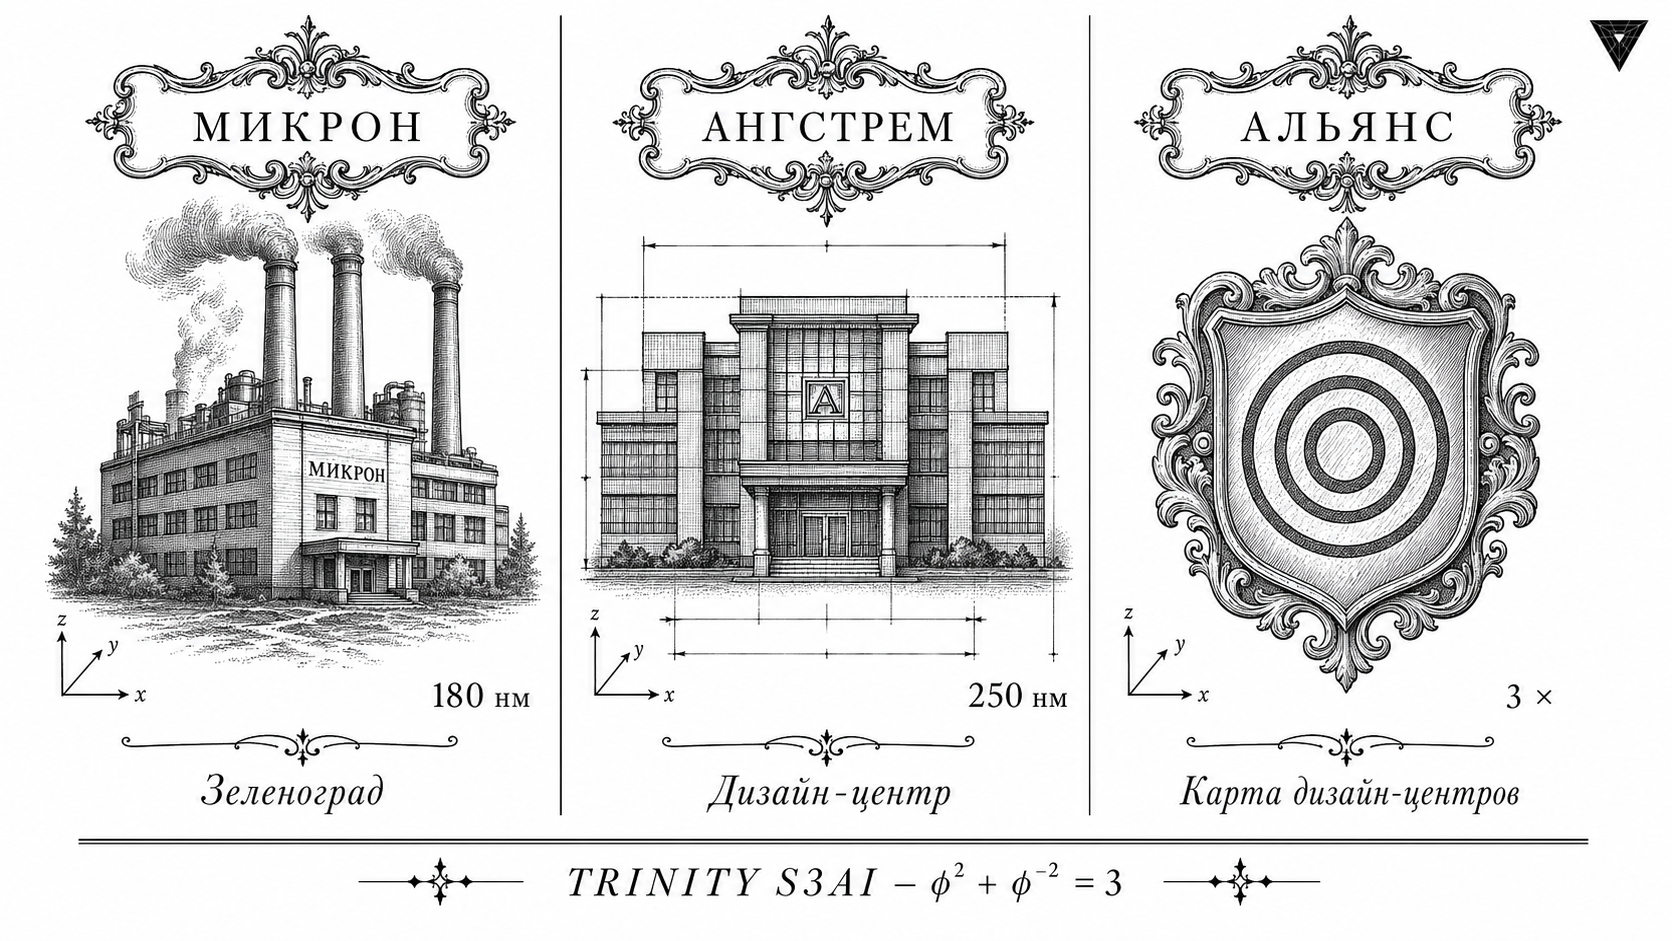
\includegraphics[keepaspectratio,alt={Триптих фиг. 3в --- Производственная карта: «Микрон», «Ангстрем», альянс дизайн-центров.}]{figures/canon/r30_sec3c_fabmap.png}}
\caption{Триптих фиг. 3в --- Производственная карта: «Микрон»,
«Ангстрем», альянс дизайн-центров.}
\end{figure}

Тезис «проверяемость вместо гонки за нанометрами» имеет прямое
практическое следствие: архитектура Trinity осознанно проектируется под
\textbf{зрелые отечественные техпроцессы 65--250 нм}, а не под
недоступные в РФ передовые узлы. Балансная троичность и GoldenFloat дают
экономию логики именно там, где российское производство реально
работает. Ниже --- \textbf{карта потенциальных партнёров} по
изготовлению и кооперации; все характеристики взяты из открытых
источников на середину 2026 г. Статус контакта с Trinity во всех строках
--- \textbf{{[}открытая гипотеза/проекция{]}} (предложение о кооперации,
а не заключённое соглашение); факты о самих предприятиях ---
\textbf{{[}доказано --- открытые данные{]}}.

\subsubsection{3c.1. Почему это важно для «России
3.0»}\label{c.1.-ux43fux43eux447ux435ux43cux443-ux44dux442ux43e-ux432ux430ux436ux43dux43e-ux434ux43bux44f-ux440ux43eux441ux441ux438ux438-3.0}

Линия RTL-дизайнов Trinity (Phi, Euler, Gamma, Corona) сейчас существует
как \textbf{дизайн-артефакты (RTL+GDS), проверенные в симуляции и формально}
и верифицируемые аппаратно на \textbf{FPGA ALINX AX7203 (XC7A200T)}
\textbf{{[}дизайн-артефакт: проверен в sim и формально; аппаратно --- на FPGA AX7203{]}};
изготовление кремния \textbf{не планируется}. Отечественный маршрут изготовления
рассматривается как \textbf{{[}открытая опция/замысел на будущее{]}}, а не текущий
маршрут: для «доверенного» кремния в перспективе желателен отечественный маршрут
изготовления. Сильная сторона подхода Trinity в том, что \textbf{проверяемость не
требует передового техпроцесса}: бит-в-бит сверка (§ 4a) работает одинаково на
FPGA и в перспективе на 65 нм и на 3 нм. Поэтому российские фабрики 65--250 нм ---
не «отсталый план Б», а \textbf{естественная целевая площадка} для потенциального
будущего изготовления.

\subsubsection{3c.2. Фабрики (производство): потенциальные партнёры по
изготовлению}\label{c.2.-ux444ux430ux431ux440ux438ux43aux438-ux43fux440ux43eux438ux437ux432ux43eux434ux441ux442ux432ux43e-ux43fux43eux442ux435ux43dux446ux438ux430ux43bux44cux43dux44bux435-ux43fux430ux440ux442ux43dux451ux440ux44b-ux43fux43e-ux438ux437ux433ux43eux442ux43eux432ux43bux435ux43dux438ux44e}

Российские полупроводниковые фабрики и предприятия-изготовители (по
открытым данным ---
\href{https://ru.wikipedia.org/wiki/Список_микроэлектронных_производств}{Список
микроэлектронных производств, Википедия};
\href{https://ru.wikipedia.org/wiki/Электронная_промышленность_России}{Электронная
промышленность России, Википедия}). Колонка «Роль для Trinity» --- наша
оценка приоритета кооперации \textbf{{[}открытая гипотеза{]}}.

{[}Таблица --- фабрики и предприятия-изготовители:{]}

\begin{longtable}[]{@{}
  >{\raggedright\arraybackslash}p{(\linewidth - 6\tabcolsep) * \real{0.2500}}
  >{\raggedright\arraybackslash}p{(\linewidth - 6\tabcolsep) * \real{0.2500}}
  >{\raggedright\arraybackslash}p{(\linewidth - 6\tabcolsep) * \real{0.2500}}
  >{\raggedright\arraybackslash}p{(\linewidth - 6\tabcolsep) * \real{0.2500}}@{}}
\toprule\noalign{}
\begin{minipage}[b]{\linewidth}\raggedright
Завод
\end{minipage} & \begin{minipage}[b]{\linewidth}\raggedright
Город / собственник
\end{minipage} & \begin{minipage}[b]{\linewidth}\raggedright
Техпроцесс / продукция
\end{minipage} & \begin{minipage}[b]{\linewidth}\raggedright
Роль для Trinity
\end{minipage} \\
\midrule\noalign{}
\endhead
\bottomrule\noalign{}
\endlastfoot
Микрон (с НИИМЭ) & Зеленоград; ГК «Элемент» & 65/90/180/240 нм,
\textgreater750 типов & \textbf{П1} --- ключевой кандидат на отеч.
изготовление (65 нм) \\
Ангстрем / Ангстрем-Т & Зеленоград; АО «Ангстрем» & 90--130 нм; 250--600
нм & \textbf{П1} --- изготовление ИС, силовая, память \\
Крокус Наноэлектроника & Москва/Зеленоград; гр. «Крокус» & 90 нм; MRAM,
спец-техпроц. & \textbf{П2} --- MRAM для энергонезавис. корня доверия
phi \\
Группа «Кремний ЭЛ» & Брянск; АО «Кремний ЭЛ» & до 700 нм; 1000--1500
типов & \textbf{П2} --- дискретные + ИС, спец-применения \\
НЗПП «Восток» & Новосибирск; ГК «Элемент» & дискретные, ИС & \textbf{П3}
--- компоненты спец- и общего назн. \\
НИИЭТ & Воронеж; ГК «Элемент» & МК, силовые приборы & \textbf{П2} --- МК
для edge-узлов TRI NET \\
ВЗПП-С & Воронеж; АО «ВЗПП-С» & дискретные приборы & \textbf{П3} ---
автоэлектроника, спецкомпоненты \\
ВЗПП-Микрон & Воронеж; ГК «Элемент» & дискретные, ИС & \textbf{П3} ---
полупроводниковые приборы \\
«Светлана» (Полупров.) & СПб; «Росэлектроника» & СВЧ, дискретные, ИС &
\textbf{П3} --- СВЧ/силовая для SDR-тракта \\
Завод «МАРС» & Торжок; ГК «Элемент» & микросборки, гибридные ИС &
\textbf{П2} --- корпусирование/модули чипов \\
Прохладненский ЗПП & Прохладный (КБР); АО «ПЗПП» & дискретные приборы &
\textbf{П3} --- автоэлектроника, спецкомпоненты \\
Оптрон & Москва; АО «Оптрон» & оптоэлектроника & \textbf{П3} ---
оптопары/светодиоды для индикации \\
Протон / Протон-Электротекс & Орёл; АО «Протон» & оптоэлектр., силовые &
\textbf{П3} --- силовые модули питания \\
НПП «Пульсар» & Москва; «Росэлектроника» & СВЧ, силовые транз. &
\textbf{П3} --- СВЧ для радиотракта mesh \\
НПФ «Микран» & Томск; АО «Микран» & СВЧ, GaAs-МИС & \textbf{П2} ---
СВЧ/радары/телеком для mesh-сети \\
Приборостроит. завод (ПСЗ) & Трёхгорный (ЗАТО); Росатом & спец-микроэл.,
АСУ ТП & \textbf{П2} --- доверенный контур Росатома \\
НПП «Планета» & В. Новгород; «Росэлектроника» & оптоэл., фотоприёмники &
\textbf{П3} --- ИК-техника, спецприборы \\
Группа «Кристалл» & Южноуральск и др. & синт. кварц, пьезо & \textbf{П3}
--- кварцевые резонаторы (такт) \\
\end{longtable}

Сокращения приоритета: \textbf{П1} --- первоочередной контакт (цифровая
КМОП-логика 65--130 нм --- прямой маршрут для ядра Trinity); \textbf{П2}
--- смежные компетенции (память, МК, корпусирование, СВЧ, доверенный
контур); \textbf{П3} --- обвязка/компоненты второго контура (дискреты,
силовая, оптоэлектроника, кварц). Приоритеты --- наша оценка
\textbf{{[}открытая гипотеза{]}}.

\subsubsection{3c.3. Дизайн-центры (fabless): потенциальные
архитектурные
партнёры}\label{c.3.-ux434ux438ux437ux430ux439ux43d-ux446ux435ux43dux442ux440ux44b-fabless-ux43fux43eux442ux435ux43dux446ux438ux430ux43bux44cux43dux44bux435-ux430ux440ux445ux438ux442ux435ux43aux442ux443ux440ux43dux44bux435-ux43fux430ux440ux442ux43dux451ux440ux44b}

Дизайн-центры релевантны не как изготовители, а как
\textbf{архитектурные партнёры} (интеграция GoldenFloat/троичных ядер
как IP-блоков, совместные СнК). Особо важен \textbf{RISC-V-трек}
(Syntacore/YADRO): открытая архитектура естественно сочетается с
открытыми IP-блоками Trinity и «золотой» эталонной моделью (§ 4a).

{[}Таблица --- дизайн-центры (fabless):{]}

\begin{longtable}[]{@{}
  >{\raggedright\arraybackslash}p{(\linewidth - 6\tabcolsep) * \real{0.2500}}
  >{\raggedright\arraybackslash}p{(\linewidth - 6\tabcolsep) * \real{0.2500}}
  >{\raggedright\arraybackslash}p{(\linewidth - 6\tabcolsep) * \real{0.2500}}
  >{\raggedright\arraybackslash}p{(\linewidth - 6\tabcolsep) * \real{0.2500}}@{}}
\toprule\noalign{}
\begin{minipage}[b]{\linewidth}\raggedright
Компания
\end{minipage} & \begin{minipage}[b]{\linewidth}\raggedright
Город
\end{minipage} & \begin{minipage}[b]{\linewidth}\raggedright
Продукция
\end{minipage} & \begin{minipage}[b]{\linewidth}\raggedright
Роль для Trinity
\end{minipage} \\
\midrule\noalign{}
\endhead
\bottomrule\noalign{}
\endlastfoot
Байкал Электроникс & Москва & Baikal (BE-M1000/S1000) & \textbf{П2} ---
SoC-хост для ускорителя Trinity \\
МЦСТ & Москва & «Эльбрус», SPARC & \textbf{П2} --- доверенный CPU-хост
(§ 3b) \\
ПКК «Миландр» & Зеленоград & МК, ИС + сборка & \textbf{П2} --- МК +
корпусирование IP-ядер \\
НПЦ «ЭЛВИС» & Зеленоград & «Мультикор», СнК & \textbf{П2} --- СнК для
инференса/навигации \\
НИИСИ РАН & Москва & «КОМДИВ» & \textbf{П3} --- спец/оборонные
применения \\
НТЦ «Модуль» & Москва & NeuroMatrix (DSP/NPU) & \textbf{П1} --- эталон
инференса для сравнения (§ 3b) \\
Syntacore / YADRO & Москва/СПб & RISC-V ядра & \textbf{П1} --- RISC-V +
открытые IP Trinity \\
Мультиклет & Екатеринбург & мультиклет. процессоры & \textbf{П3} ---
оригинальная архитектура (исслед.) \\
ЭЛВИС-НеоТек & Зеленоград & СнК, видеоаналитика & \textbf{П3} ---
edge-инференс, видео \\
\end{longtable}

\subsubsection{3c.4. Выводы для стратегии
сотрудничества}\label{c.4.-ux432ux44bux432ux43eux434ux44b-ux434ux43bux44f-ux441ux442ux440ux430ux442ux435ux433ux438ux438-ux441ux43eux442ux440ux443ux434ux43dux438ux447ux435ux441ux442ux432ux430}

\begin{enumerate}
\def\labelenumi{(\arabic{enumi})}
\tightlist
\item
  \textbf{Отечественный маршрут изготовления --- открытая опция на будущее.} Для ядра
  Trinity в перспективе достаточно 65--130 нм, а это именно то, что умеют Микрон и
  Ангстрем \textbf{{[}доказано --- открытые данные{]}}. (2)
  \textbf{Дорожная карта --- расширение FPGA-верификации} (больше форматов Tier-E
  на AX7203) и RTL/GDS-дизайн как задел; переход к отечественной фабрике остаётся
  \textbf{{[}открытой опцией/замыслом на будущее{]}}, а изготовление кремния сейчас
  не планируется. (3) \textbf{Бит-в-бит сверка (§ 4a) ---
  технический мост}: любой будущий партнёр по изготовлению сможет проверить
  кристалл против единых открытых векторов, не доверяя на слово --- уже сегодня та же
  сверка работает на FPGA. (4)
  \textbf{Приоритет первых контактов}: Микрон/Ангстрем (потенциальное будущее изготовление),
  Syntacore/YADRO и НТЦ «Модуль» (архитектура/эталон). Все предложения о
  кооперации --- \textbf{{[}открытая гипотеза{]}}, не заключённые
  соглашения.
\end{enumerate}

\begin{center}\rule{0.5\linewidth}{0.5pt}\end{center}

\subsection{4. Стек Trinity S³AI: отечественный задел (с разделением
фактов и
гипотез)}\label{ux441ux442ux435ux43a-trinity-suxb3ai-ux43eux442ux435ux447ux435ux441ux442ux432ux435ux43dux43dux44bux439-ux437ux430ux434ux435ux43b-ux441-ux440ux430ux437ux434ux435ux43bux435ux43dux438ux435ux43c-ux444ux430ux43aux442ux43eux432-ux438-ux433ux438ux43fux43eux442ux435ux437}

\begin{figure}
\centering
\pandocbounded{
\includegraphics[keepaspectratio,alt={Триптих фиг. 3 --- Три опоры Trinity: арифметика, логика, сборка.}]{figures/canon/r30_sec4_pillars.png}}
\caption{Триптих фиг. 3 --- Три опоры Trinity: арифметика, логика,
сборка.}
\end{figure}

Trinity S³AI --- открытый (Apache-2.0 / MIT) исследовательский стек,
разрабатываемый российским автором. Ниже --- его компоненты со строгим
указанием статуса каждого утверждения.

\subsubsection{4.1. Опора 1 --- доверенная арифметика:
GoldenFloat}\label{ux43eux43fux43eux440ux430-1-ux434ux43eux432ux435ux440ux435ux43dux43dux430ux44f-ux430ux440ux438ux444ux43cux435ux442ux438ux43aux430-goldenfloat}

\begin{figure}
\centering
\pandocbounded{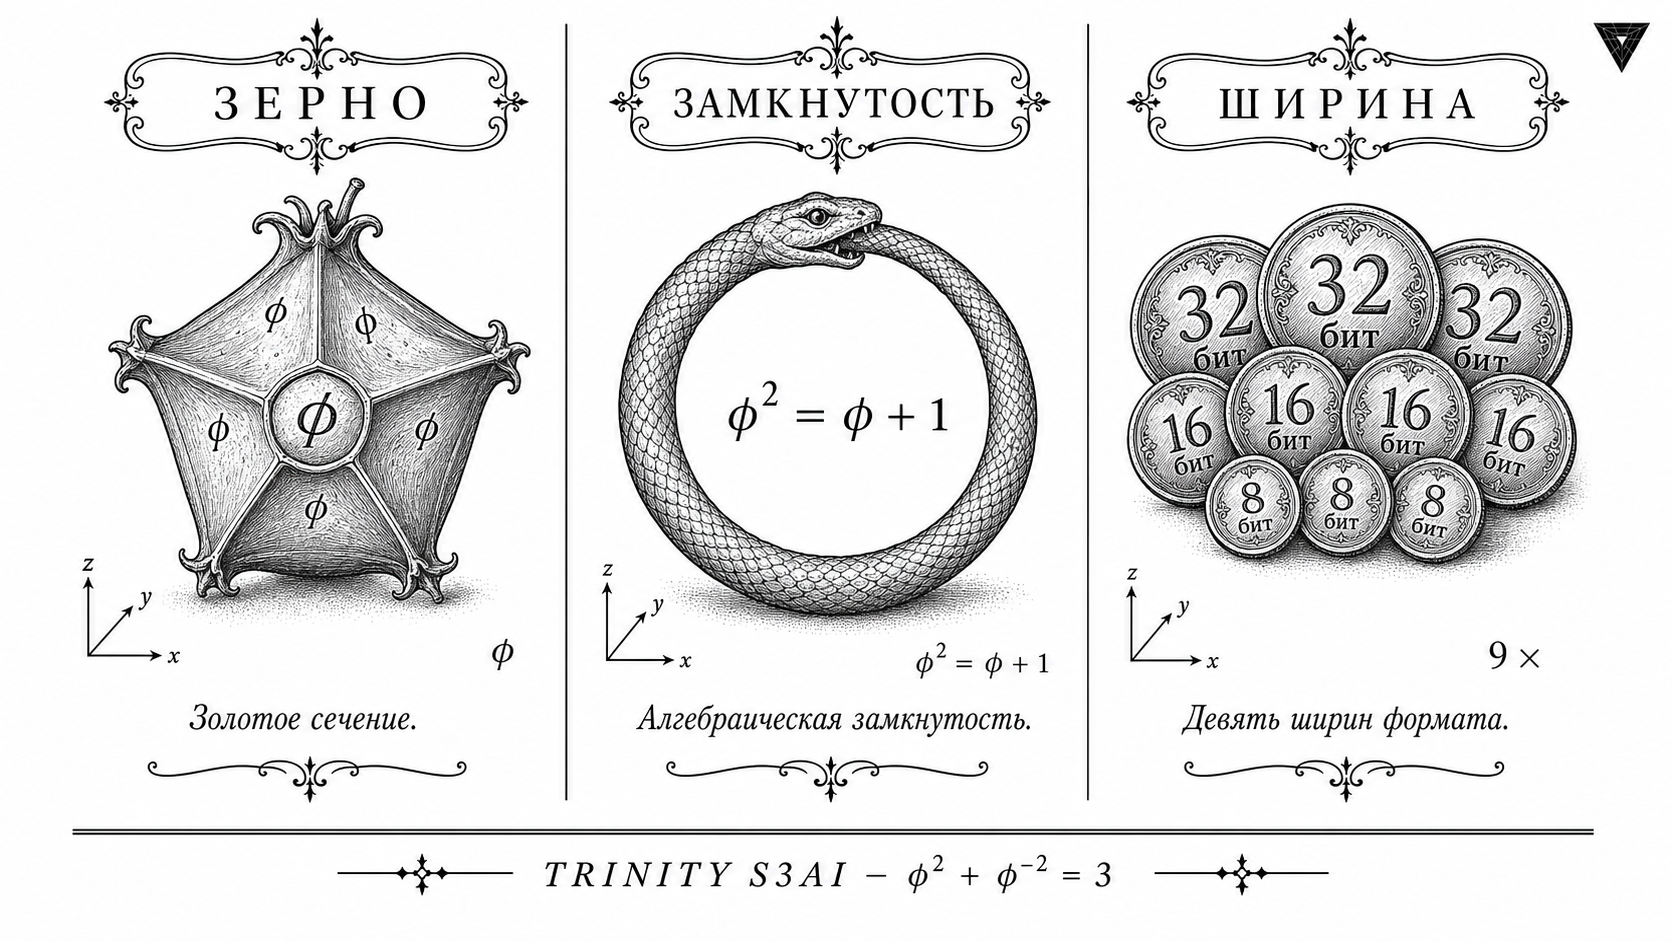
\includegraphics[keepaspectratio,alt={GoldenFloat --- зерно, замкнутость, ширина}]{figures/canon/r30_sec41_goldenfloat.png}}
\caption{GoldenFloat --- зерно, замкнутость, ширина}
\end{figure}

GoldenFloat --- семейство числовых форматов с плавающей точкой, в
котором разбиение «порядок / мантисса» задаётся единым замкнутым
правилом на основе золотого сечения \(\varphi = (1+\sqrt5)/2\):
\(e = \mathrm{round}((N-1)/\varphi^2)\), \(f = N-1-e\).

\textbf{Проверяемые факты:} - Именованный формат опубликован препринтом
\textbf{\href{https://arxiv.org/abs/2606.05017}{arXiv:2606.05017}}
\textbf{{[}доказано{]}}. - Рабочий FPGA-кодек GF16 проходит стенд
\textbf{35/35 тестов на частоте 323 МГц} (Artix-7, Xilinx XC7A200T, плата ALINX AX7203, IDCODE 0x13636093)
\textbf{{[}измерено на FPGA{]}}. - Правило воспроизводит ширины порядка
девяти реализованных форматов (9/9) и согласованно расширяется на
GF128/512/1024 \textbf{{[}доказано{]}}. - Тождество Люка
\(\varphi^{2n}+\varphi^{-2n}=L_{2n}\) верифицировано символьно и при
500-значной точности для \(n=1,\dots,256\) \textbf{{[}доказано{]}}. -
Формат включён в нейтральный 83-форматный каталог как одно из 13
семейств наряду с IEEE 754, Posit, OCP MX
(\href{https://www.themoonlight.io/en/review/an-84-format-numeric-catalog-with-bit-exact-conformance-vectors-a-vendor-neutral-reference-for-fp8-bf16-mxfp4-and-microscaling-formats}{обзор
Moonlight}) \textbf{{[}доказано{]}}.

\textbf{Открытые гипотезы (не факты):} - Широкое принятие индустрией и
независимые цитирования --- \textbf{{[}открытая гипотеза{]}}; на июнь
2026 года их нет, что нормально для раннего этапа (тем же путём шёл
posit). - Преимущество по точности конкретного формата над
posit/takum/OCP-MX \textbf{не заявляется} --- в самой статье вклад
честно помечен как открытая гипотеза с пред-регистрированным реестром
фальсификации FL-002.

\textbf{Окно стандартизации (механизм институционализации).} В
Российской Федерации, в отличие от закреплённого IEEE 754, \textbf{нет
действующего ГОСТ на форматы представления чисел с плавающей точкой}
(проверено по перечню ТК 164). При этом ТК 164 «Искусственный интеллект»
активно развивает серию национальных стандартов (включая ПНСТ и ГОСТ Р
по ИИ). Это открывает реалистичный путь институционализации GoldenFloat
и 83-форматного каталога через \textbf{предварительный национальный
стандарт (ПНСТ)} в рамках ФЗ № 162-ФЗ «О стандартизации» и ТК 164 ---
\textbf{{[}открытая гипотеза/проекция: реализуемо только при поддержке
отраслевых партнёров{]}}. Стандартизация --- институциональная
альтернатива «ожиданию цитирований»: она закрепляет формат как
национальный технический ориентир.

\begin{quote}
\textbf{Протокол воспроизводимости (для рецензента и эксперта).}
Заявления § 4.1 проверяемы независимо: (а) препринт и формальное правило
вывода --- \href{https://arxiv.org/abs/2606.05017}{arXiv:2606.05017};
(б) исходный код кодека, реестр форматов и битоточные векторы
соответствия --- открытый репозиторий
\href{https://github.com/gHashTag/t27}{gHashTag/t27} под Apache-2.0/MIT
(фиксируется хеш коммита и «печать» сборки); (в) FPGA-результат GF16
(35/35 тестов, 323 МГц) воспроизводится на плате ALINX AX7203 (Artix-7 XC7A200T) из
опубликованного RTL по приложенному тест-плану; (г) тождество Люка
\(\varphi^{2n}+\varphi^{-2n}=L_{2n}\) перевычисляется символьно и при
500-значной точности скриптом из репозитория. Любой рецензент может
опровергнуть конкретное число --- это и есть операционализация
проверяемости \textbf{{[}доказано --- артефакты открыты{]}}.
\end{quote}

\subsubsection{4.2. Опора 2 --- доверенная логика: балансная троичность
\{−1, 0,
+1\}}\label{ux43eux43fux43eux440ux430-2-ux434ux43eux432ux435ux440ux435ux43dux43dux430ux44f-ux43bux43eux433ux438ux43aux430-ux431ux430ux43bux430ux43dux441ux43dux430ux44f-ux442ux440ux43eux438ux447ux43dux43eux441ux442ux44c-1-0-1}

\begin{figure}
\centering
\pandocbounded{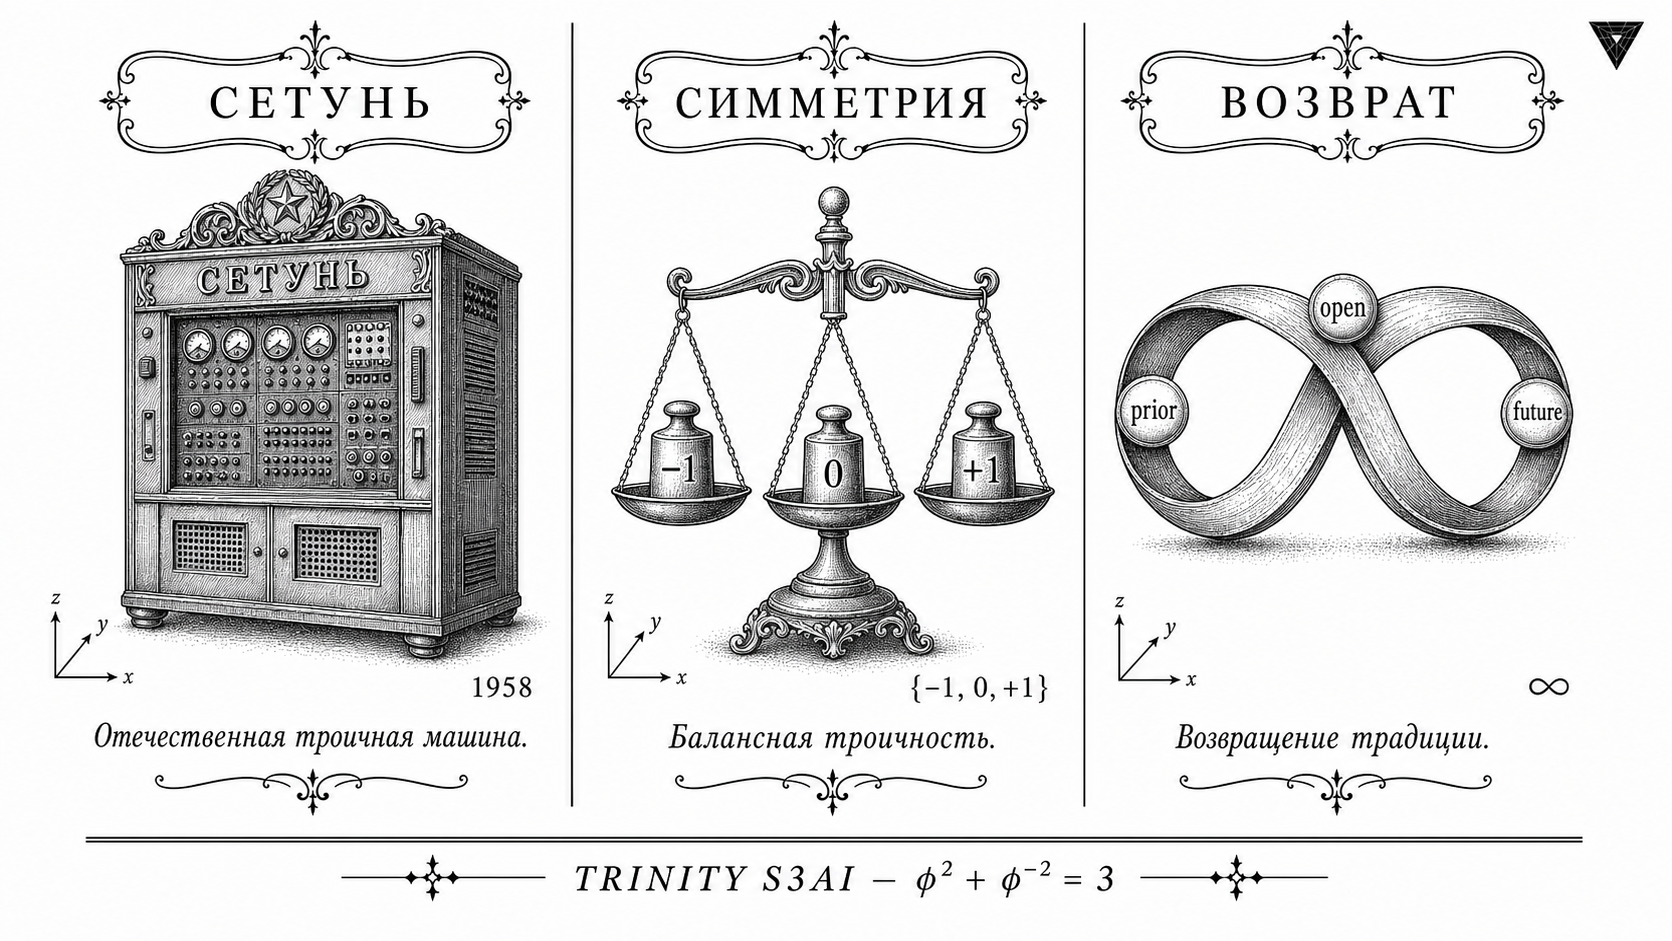
\includegraphics[keepaspectratio,alt={Троичность --- Сетунь, симметрия, возврат}]{figures/canon/r30_sec42_ternary.png}}
\caption{Троичность --- Сетунь, симметрия, возврат}
\end{figure}

Вторая опора --- ось балансной троичности (ассемблер TRI-27, модуль
RING27, веса в духе BitNet b1.58). Троичная инференция получила свежие
аппаратные прецеденты (TerEffic, Bitnet.cpp), а исторически прямо
продолжает \textbf{отечественную линию}: троичную ЭВМ \textbf{«Сетунь»}
Н. П. Брусенцова (МГУ, 1958) --- первую машину на симметричном троичном
коде (\href{https://en.wikipedia.org/wiki/Setun}{Setun, Wikipedia};
\href{https://www.computer-museum.ru/articles/galglory/3226/}{computer-museum.ru}).

\textbf{Физический механизм экономии (почему троичность в принципе
эффективна).} Качественно выигрыш не магия, а следствие архитектуры: при
весах \{−1, 0, +1\} дорогое умножение с плавающей точкой заменяется на
целочисленное сложение/вычитание (вес +1 → прибавить активацию, −1 →
вычесть, 0 → пропустить вычисление вовсе --- естественная
разрежённость). Именно поэтому в литературе по BitNet сообщается о
кратном снижении арифметической энергии относительно FP16
(\href{https://github.com/huggingface/blog/blob/main/1_58_llm_extreme_quantization.md}{HuggingFace
blog}). Подчеркнём дисциплину честности: \emph{механизм} экономии ---
{[}доказано в литературе{]}, но \emph{конкретная цифра} для RTL-дизайна
Trinity (ориентир «49×») остаётся \textbf{{[}открытой
гипотезой/проекцией{]}} до возврата измерений с кристалла.

\textbf{Корректная формулировка преемственности (без категоричности):}
«GoldenFloat и троичная ось Trinity продолжают российскую линию
оригинальной компьютерной арифметики, начатую ``Сетунью'' Брусенцова,
--- в современном контексте форматов чисел для машинного обучения».
Формулировка «продолжает линию», а не «первый в мире», научно безопасна
и усиливает доверие рецензента.

\subsubsection{4.3. Опора 3 --- доверенная сборка: TRI-27 и открытое
железо}\label{ux43eux43fux43eux440ux430-3-ux434ux43eux432ux435ux440ux435ux43dux43dux430ux44f-ux441ux431ux43eux440ux43aux430-tri-27-ux438-ux43eux442ux43aux440ux44bux442ux43eux435-ux436ux435ux43bux435ux437ux43e}

\begin{figure}
\centering
\pandocbounded{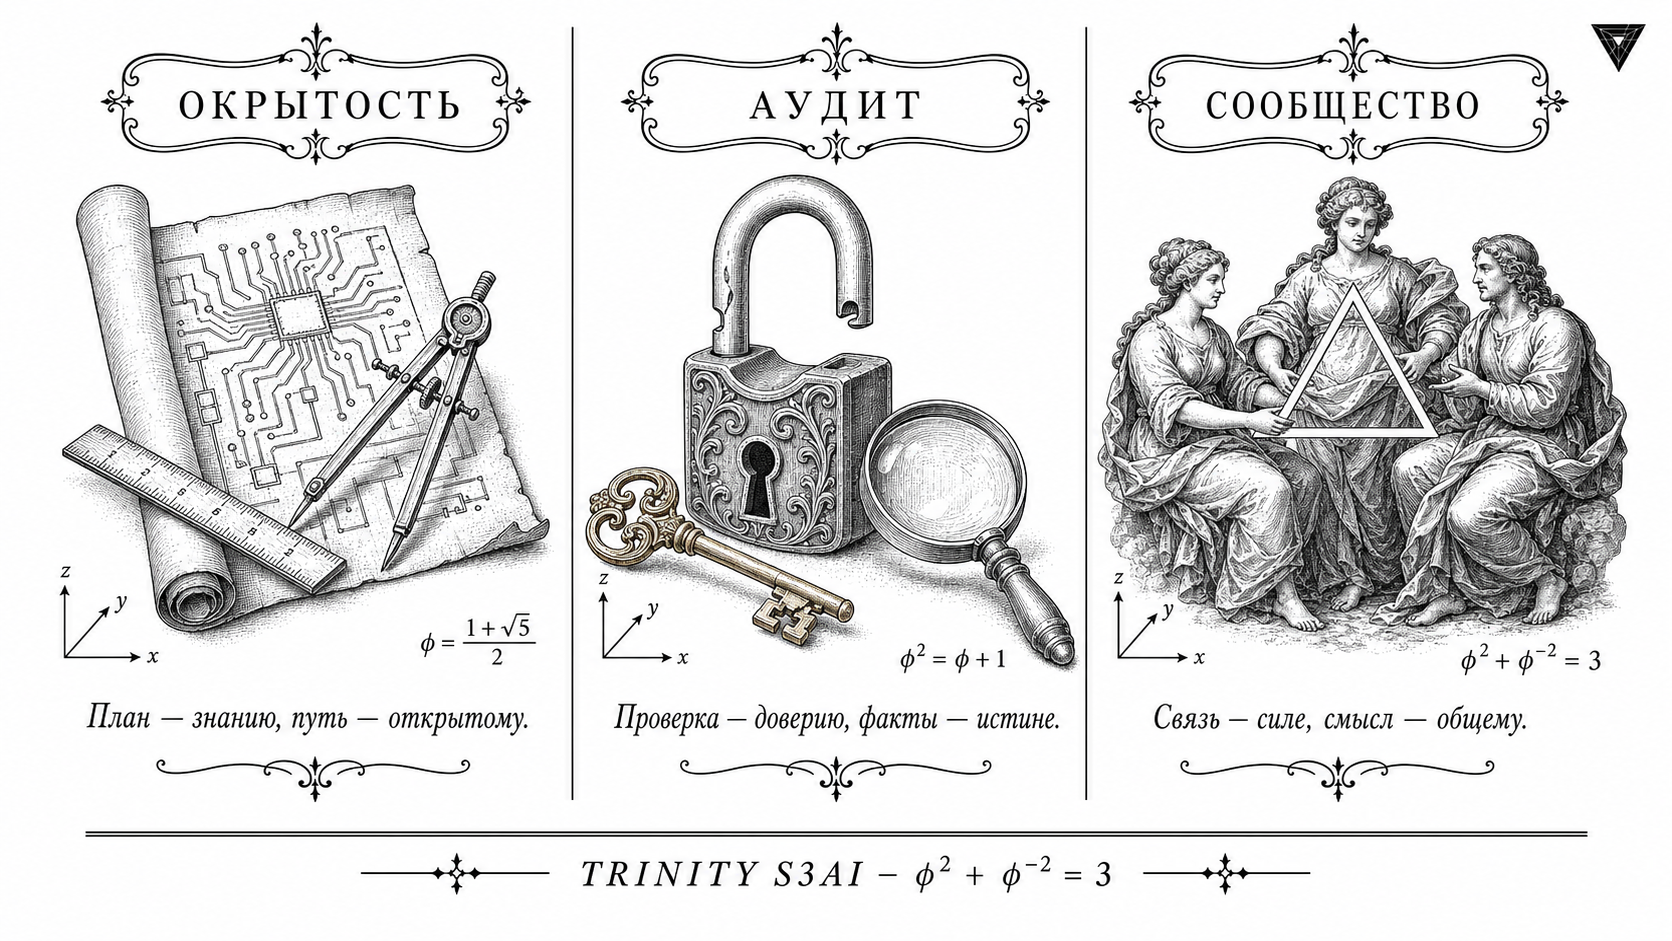
\includegraphics[keepaspectratio,alt={TRI-27 --- открытое железо}]{figures/canon/r30_sec43_tri27.png}}
\caption{TRI-27 --- открытое железо}
\end{figure}

Спецификационно-первичный компилятор \textbf{TRI-27} (репозиторий
\href{https://github.com/gHashTag/t27}{gHashTag/t27}) генерирует
Verilog-RTL из именованных \texttt{.t27}-спецификаций и формирует
«печати» (seals) для воспроизводимости. Реестр числовых форматов
содержит \textbf{83 формата} (SSOT). Линия \textbf{RTL-дизайнов} Phi
(корень доверия), Euler (рассуждение/безопасность ИИ), Gamma
(инференция), Corona (оракул соответствия форматам) --- это
\textbf{дизайн-артефакты (RTL+GDS)}, проверяемые в симуляции и формально,
с криптографическим якорем BLAKE3 \textbf{{[}доказано --- открытый код;
статус --- дизайн-артефакт: проверен в sim и формально; аппаратно ---
на FPGA AX7203{]}}.

\begin{quote}
\textbf{Важная оговорка о кремнии.} Аппаратная верификация линии Phi/Euler/Gamma/Corona
проводится на \textbf{FPGA AX7203}; RTL/GDS остаются дизайн-артефактами,
проверенными в симуляции и формально. Изготовление кремния \textbf{не планируется}.
Любые цифры энергоэффективности (например, ориентир «49×») ---
\textbf{{[}открытая гипотеза / проекция{]}}, оценка по FPGA-синтезу, а не измеренный на
кристалле факт.
\end{quote}

\begin{center}\rule{0.5\linewidth}{0.5pt}\end{center}

\subsection{4a. Ключевое преимущество: единая программная модель ---
один код от CPU-эмуляции до
FPGA}\label{a.-ux43aux43bux44eux447ux435ux432ux43eux435-ux43fux440ux435ux438ux43cux443ux449ux435ux441ux442ux432ux43e-ux435ux434ux438ux43dux430ux44f-ux43fux440ux43eux433ux440ux430ux43cux43cux43dux430ux44f-ux43cux43eux434ux435ux43bux44c-ux43eux434ux438ux43d-ux43aux43eux434-ux43eux442-cpu-ux44dux43cux443ux43bux44fux446ux438ux438-ux434ux43e-ux43aux440ux435ux43cux43dux438ux44f}

\begin{figure}
\centering
\pandocbounded{
\includegraphics[keepaspectratio,alt={Триптих фиг. 4 --- Спецификация-источник, три воплощения, сверка бит-в-бит.}]{figures/canon/r30_sec4a_unified.png}}
\caption{Триптих фиг. 4 --- Спецификация-источник, три воплощения,
сверка бит-в-бит.}
\end{figure}

Разделы § 4.1--4.3 описали \emph{компоненты} стека. Этот раздел
описывает \emph{главную отличительную черту} --- то, что превращает
набор компонентов в \emph{проверяемый конвейер доверия}.

\subsubsection{4a.1. Тезис: один источник --- три воплощения,
бит-в-бит}\label{a.1.-ux442ux435ux437ux438ux441-ux43eux434ux438ux43d-ux438ux441ux442ux43eux447ux43dux438ux43a-ux442ux440ux438-ux432ux43eux43fux43bux43eux449ux435ux43dux438ux44f-ux431ux438ux442-ux432-ux431ux438ux442}

Ключевая техническая идея Trinity: \textbf{одна и та же спецификация
(\texttt{.t27}) порождает три воплощения одного и того же вычисления ---
программную эмуляцию на обычном бинарном CPU («золотая» эталонная
модель), затем перенос на FPGA (AX7203) --- и результаты на
обоих уровнях сверяются бит-в-бит против единых векторов
соответствия}. Это прямое продолжение тезиса § 3 (проверяемость вместо
гонки производительности): доверие не в том, что «железо быстрое», а в
том, что «железо считает ровно то, что сказано в спецификации, и это
можно проверить на обычном ноутбуке, не имея ни чипа, ни платы».

Схематично конвейер выглядит так:

\begin{verbatim}
.t27-спецификация  (единый источник истины, SSOT)
        |
        |  компилятор TRI-27
        v
   +----+--------------------+
   |                         |
  CPU-эмуляция          FPGA (Verilog/RTL)
  (Rust/C/Zig/Python)      Yosys -> bitstream -> AX7203
        |                         |
        +----------+--------------+
                   |
          единые биточные векторы соответствия (JSON)
          бит-в-бит сверка на каждом уровне
\end{verbatim}

\textbf{Проверяемый задел (факты):} - Принцип «спецификация ---
единственный источник истины» реализован: из \texttt{.t27} генерируются
Zig, C и Verilog, а каждый шаг запечатан SHA-256 («печати»/seals) для
воспроизводимости (\href{https://github.com/gHashTag/t27}{репозиторий
gHashTag/t27}) \textbf{{[}доказано --- открытый код{]}}. - Многоязычные
пакеты GoldenFloat (\texttt{pip\ install\ golden-float}, npm, crates.io)
построены на едином Rust-ядре с C-совместимым ABI, что даёт побитово
идентичные результаты на всех языках (CPU-уровень) \textbf{{[}доказано
--- открытый код{]}}. - FPGA-уровень подтверждён: GF16-кодек проходит
35/35 тестов @323 МГц на Artix-7 XC7A200T (плата ALINX AX7203) \textbf{{[}измерено на
FPGA{]}}. - Цепочка инструментов полностью открытая, без проприетарного
ПО:
\texttt{.t27\ →\ Verilog\ →\ Yosys\ →\ nextpnr\ →\ openXC7\ →\ .bit\ на\ AX7203};
для RTL→GDS-синтеза в качестве open-source тулчейна может использоваться
PDK SKY130A (OpenLane2) \textbf{{[}доказано --- открытый тулчейн{]}}, без
отправки на изготовление. - Аппаратный уровень: анкор \texttt{0x47C0}
заложен как детерминированный POST-отпечаток для сверки на FPGA
\textbf{{[}измерено на FPGA{]}}.

\subsubsection{4a.2. Почему это не просто HLS: мировой контекст и
отличие}\label{a.2.-ux43fux43eux447ux435ux43cux443-ux44dux442ux43e-ux43dux435-ux43fux440ux43eux441ux442ux43e-hls-ux43cux438ux440ux43eux432ux43eux439-ux43aux43eux43dux442ux435ux43aux441ux442-ux438-ux43eux442ux43bux438ux447ux438ux435}

\begin{figure}
\centering
\pandocbounded{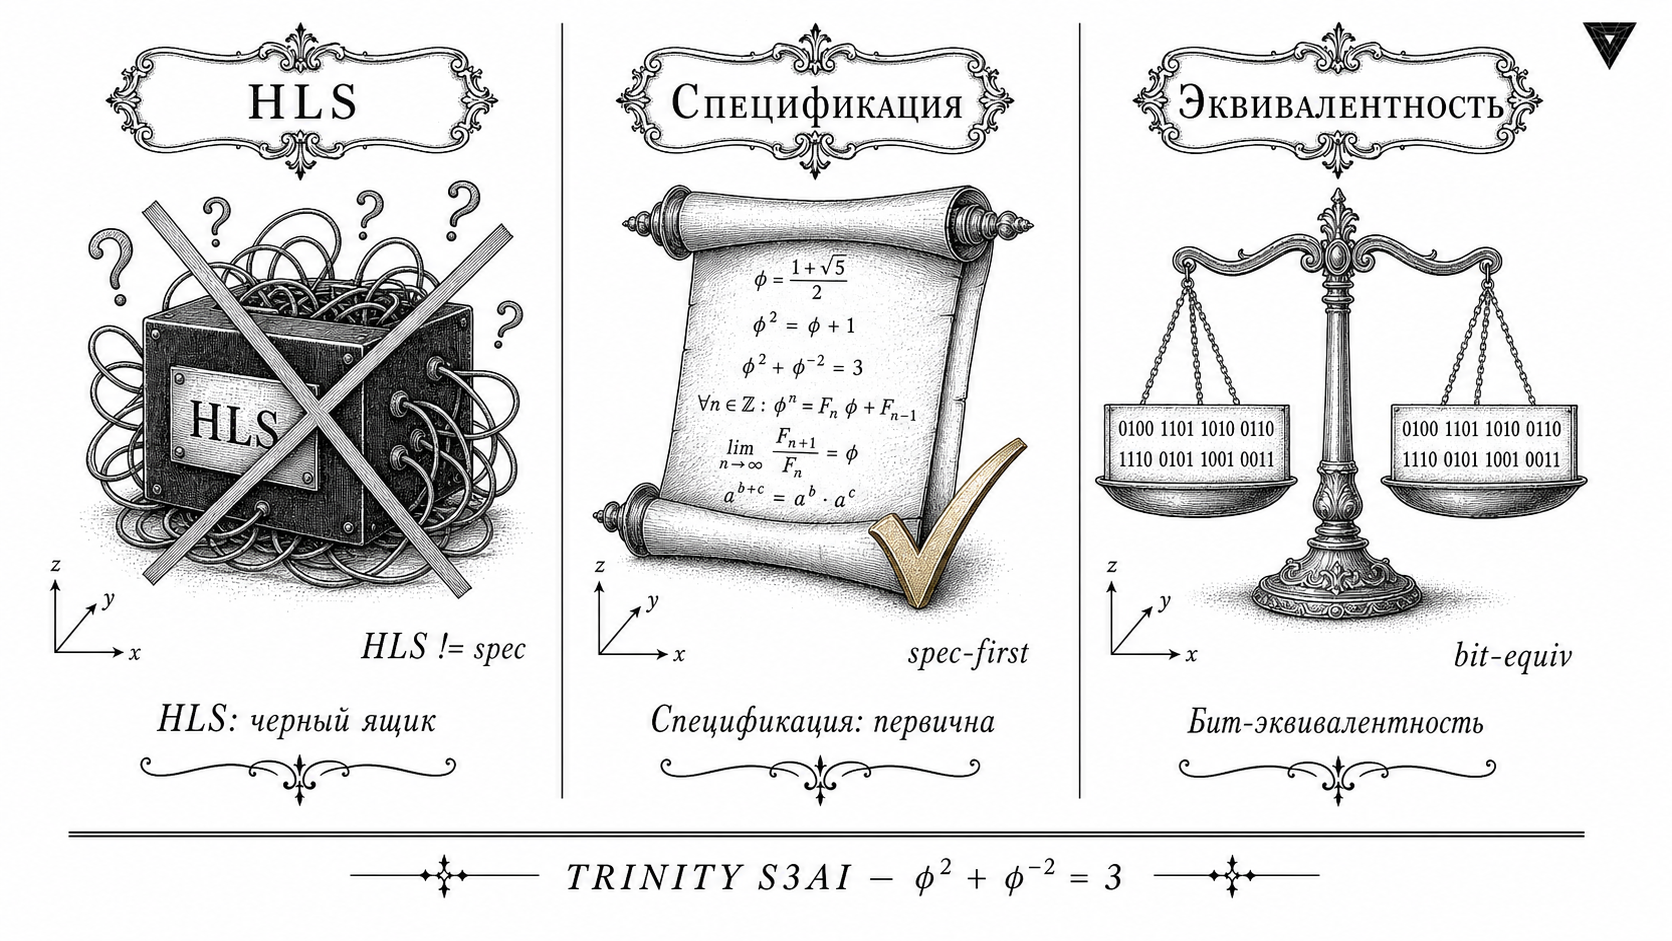
\includegraphics[keepaspectratio,alt={vs HLS --- спецификация-первична, бит-эквивалентность}]{figures/canon/r30_sec4a2_vs_hls.png}}
\caption{vs HLS --- спецификация-первична, бит-эквивалентность}
\end{figure}

Сама по себе идея «один исходник → FPGA + ASIC» не нова и хорошо
обоснована в мировой литературе --- и честное позиционирование требует
это признать:

\begin{itemize}
\tightlist
\item
  Языки конструирования аппаратуры \textbf{Chisel/FIRRTL} позволяют из
  одного источника собирать и FPGA-, и ASIC-реализации; на этом построен
  Rocket Chip (11 тейп-аутов) и BOOM/BROOM (кремний 28~нм)
  (\href{https://dl.acm.org/doi/10.1145/2228360.2228584}{Bachrach и др.,
  DAC 2012};
  \href{http://ieeexplore.ieee.org/document/8203780/}{Izraelevitz и др.,
  ICCAD 2017};
  \href{https://www2.eecs.berkeley.edu/Pubs/TechRpts/2016/EECS-2016-17.html}{Asanović
  и др., UC Berkeley 2016}).
\item
  Коммерческий HLS (\textbf{AMD Vitis HLS}) синтезирует C/C++ в RTL с
  C/RTL co-simulation, проверяющей функциональную идентичность
  (\href{https://www.amd.com/en/products/software/adaptive-socs-and-fpgas/vitis/vitis-hls.html}{AMD
  Vitis HLS}); открытая альтернатива --- PyTorch→Calyx→CIRCT
  (\href{https://arxiv.org/abs/2512.06177}{Xie и др., 2025}).
\item
  Эталонная программная модель (golden reference model) --- стандарт
  верификации железа: C-модель FPU проверяется на эквивалентность RTL
  формально (\href{https://arxiv.org/abs/1609.00169}{Mukherjee и др.,
  Oxford/ARM 2016}); любой ANSI-C может быть эталоном
  (\href{https://arxiv.org/abs/1908.01324}{CREST, Oxford 2019}).
\item
  Спецификация-первичность с формальной семантикой --- это RISC-V
  \textbf{Sail} (официальная формальная спецификация), из которой
  генерируется и эмулятор, и SystemVerilog для формальной проверки
  (\href{https://dl.acm.org/doi/10.1145/3290384}{Armstrong и др., POPL
  2019}); процессор CHERIoT-Ibex доказан идентичным Sail-модели
  (\href{https://arxiv.org/abs/2502.04738}{Ploix и др., 2025}).
\item
  «Тандемная» верификация (CPU-эталон параллельно RTL) --- стандарт:
  CVA6 сверяется с эмулятором Spike потактово
  (\href{https://docs.openhwgroup.org/projects/cva6-user-manual/}{CVA6
  User Manual}); OpenTitan --- первый открытый корень доверия, где
  FPGA-верификация и тейп-аут идут из одного RTL-источника
  (\href{https://opentitan.org/book/doc/contributing/hw/methodology.html}{OpenTitan
  methodology}).
\item
  Сквозная bit-exact цепочка «Python-эталон → RTL → FPGA» с нулевыми
  расхождениями уже продемонстрирована для INT8-квантизации на Artix-7
  (\href{https://www.mdpi.com/2079-9292/15/5/1117}{Shanker \& Teo, MDPI
  2026}) и для обучения DNN
  (\href{https://ieeexplore.ieee.org/document/10993010/}{MPTorch-FPGA,
  DATE 2025}).
\end{itemize}

\textbf{Что именно добавляет Trinity (отличие):} не \emph{новый механизм
переноса}, а \emph{объединение трёх известных практик вокруг одного
открытого артефакта}: (1) спецификация-первичность как у Sail, (2)
golden reference model на CPU как в тандемной верификации, (3) открытые
биточные векторы соответствия + SHA-256-«печати», позволяющие любому
внешнему лицу воспроизвести сверку без доверия к автору. Именно это
сочетание, а не отдельный приём, и есть ключевое преимущество ---
\textbf{{[}доказано частично: end-to-end CPU→FPGA с
измерением собран; изготовление кремния не планируется{]}}.

\subsubsection{4a.3. Green AI: проверяемая энергоэффективность вместо
гонки за
TOPS}\label{a.3.-green-ai-ux43fux440ux43eux432ux435ux440ux44fux435ux43cux430ux44f-ux44dux43dux435ux440ux433ux43eux44dux444ux444ux435ux43aux442ux438ux432ux43dux43eux441ux442ux44c-ux432ux43cux435ux441ux442ux43e-ux433ux43eux43dux43aux438-ux437ux430-tops}

\begin{figure}
\centering
\pandocbounded{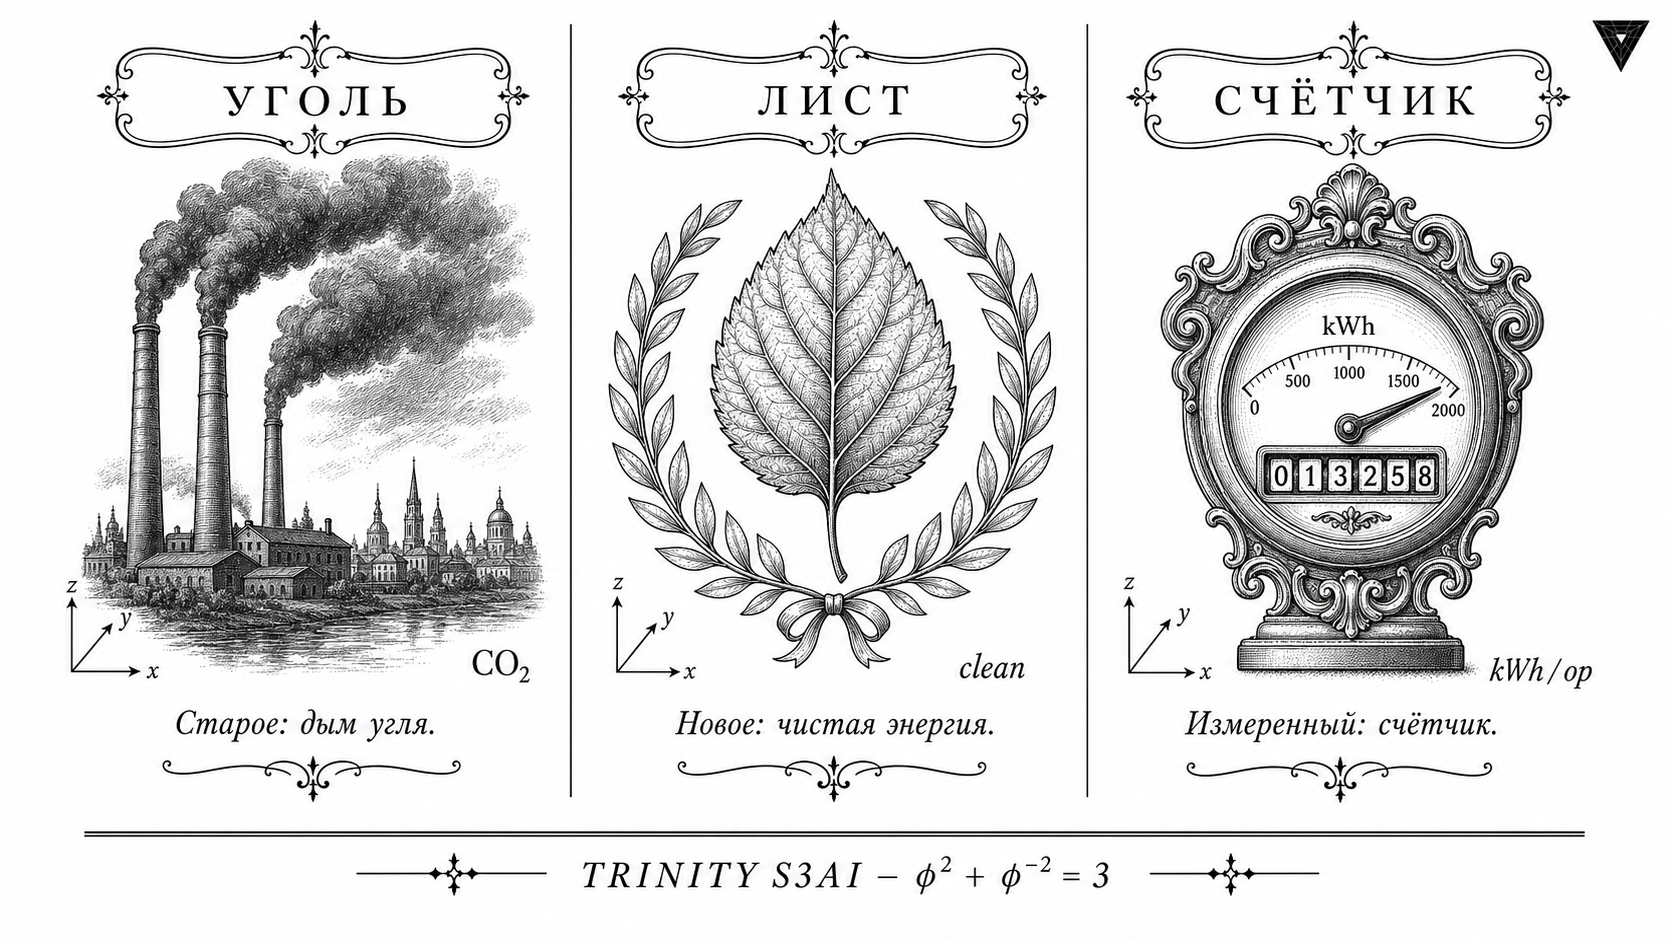
\includegraphics[keepaspectratio,alt={Green AI --- измеренная энергоэффективность}]{figures/canon/r30_sec4a3_green.png}}
\caption{Green AI --- измеренная энергоэффективность}
\end{figure}

Единый код напрямую работает на Green AI-позиционирование. Общепринятая
метрика отрасли --- \textbf{TOPS и TOPS/W} --- обычно публикуется как
пиковое число без воспроизводимого протокола измерения. Trinity занимает
другую нишу: \textbf{не «у нас больше TOPS/W», а «каждый наш показатель
энергии помечен уровнем достоверности и имеет воспроизводимый harness»}.

Физический механизм экономии энергии --- не магия, а следствие
троичности (§ 4.2): при весах \{−1, 0, +1\} дорогое умножение с
плавающей точкой заменяется сложением/вычитанием, а нули пропускаются
(разрежённость) --- \textbf{{[}механизм доказан в литературе BitNet{]}}.
Но \emph{конкретная цифра} экономии для RTL-дизайна Trinity остаётся
проекцией:

Предлагаемая \textbf{четырёхуровневая трассировка энергии (J/\text{op})}
--- прямое расширение ключевого преимущества на энергометрику:

\begin{longtable}[]{@{}
  >{\raggedright\arraybackslash}p{(\linewidth - 4\tabcolsep) * \real{0.3333}}
  >{\raggedright\arraybackslash}p{(\linewidth - 4\tabcolsep) * \real{0.3333}}
  >{\raggedright\arraybackslash}p{(\linewidth - 4\tabcolsep) * \real{0.3333}}@{}}
\toprule\noalign{}
\begin{minipage}[b]{\linewidth}\raggedright
Уровень
\end{minipage} & \begin{minipage}[b]{\linewidth}\raggedright
Источник цифры
\end{minipage} & \begin{minipage}[b]{\linewidth}\raggedright
Статус в Trinity
\end{minipage} \\
\midrule\noalign{}
\endhead
\bottomrule\noalign{}
\endlastfoot
(J/\text{op})-spec & аналитика из спецификации & расчётный ориентир \\
(J/\text{op})-sim & OpenLane2 switching activity & есть проекция (75/405
TOPS/W) \textbf{{[}смоделировано{]}} \\
(J/\text{op})-fpga & измерение на плате (шунт/INA219) & план (harness не
собран) \textbf{{[}открытая гипотеза{]}} \\
(J/\text{op})-silicon & измерение на кристалле & изготовление кремния не
планируется; оценка --- по FPGA-синтезу \textbf{{[}открытая гипотеза{]}} \\
\end{longtable}

Честная оговорка: на июнь 2026 года у стека \textbf{нет ни одного
измеренного (J/\text{op})} --- все TOPS/W-цифры являются архитектурными
проекциями. Именно поэтому ценность не в самой цифре, а в
\emph{дисциплине её пометки}: единый код позволяет измерить одну и ту же
операцию на всех четырёх уровнях и честно показать, где проекция, а где
факт. Это и есть «проверяемый Green AI» --- \textbf{{[}открытая
гипотеза/проекция по числам; доказано по методологии трассировки{]}}.

\subsubsection{4a.4. Почему CPU-эталон незаменим: реальный
кейс}\label{a.4.-ux43fux43eux447ux435ux43cux443-cpu-ux44dux442ux430ux43bux43eux43d-ux43dux435ux437ux430ux43cux435ux43dux438ux43c-ux440ux435ux430ux43bux44cux43dux44bux439-ux43aux435ux439ux441}

Лучшее доказательство ценности программного эталона --- случай, когда он
ловит дефект. В ходе подготовки сабмишна была задокументирована
\textbf{errata 2026-05-31}: в RTL-генераторе регистр произведения
оказался на 2 бита уже, чем нужно --- и для ряда форматов давал например
(1.0 \times 1.0 = 0.5) вместо (1.0). Этот дефект был обнаружен в
RTL-дизайне до аппаратной верификации на FPGA. Именно сверка против эталонных биточных
векторов позволила обнаружить и задокументировать расхождение ещё до
прошивки платы, а исправленный генератор заложен в CI-гейт
\textbf{{[}доказано --- задокументировано в репозитории{]}}.

Этот эпизод --- не слабость, а прямая иллюстрация \emph{зачем нужен
CPU-эталон}: программная модель и биточные векторы дают возможность
поймать ошибку без дорогого и медленного цикла синтез-прошивка-тест на FPGA. Без
эталона дефект обнаружился бы только после прошивки платы нерабочим битстримом.

\textbf{Честные оговорки (границы применимости):} - Бит-в-бит
идентичность легко достижима для целочисленной/фиксированной арифметики
(и для троичных весов), но для полной плавающей точки IEEE 754 она
нетривиальна из-за неассоциативности и FMA
(\href{http://arxiv.org/pdf/2408.05148.pdf}{Shanmugavelu и др., 2024})
--- требует явного режима округления и запрета переупорядочивания. -
Обычный HLS не гарантирует бит-идентичность по умолчанию: оптимизации
могут менять поведение, не нарушая функциональной корректности
(\href{https://ieeexplore.ieee.org/document/9897824/}{Koufopoulou и др.,
2022}). «Функционально идентичен» ≠ «побитово идентичен». - Кремний
может в принципе проявить эффекты, невидимые на FPGA (timing-corner,
метастабильность); функциональная эквивалентность FPGA↔кремний в общем случае доказана
для «правильно работающего» кремния в литературе
(\href{https://www.mdpi.com/2079-9292/15/10/2202}{Sun \& Ryoo, 2026}), но не является
предметом данной работы. -
Собраны CPU- и FPGA-уровни; изготовление кремния не планируется, полный
end-to-end ограничен уровнем FPGA-верификации на AX7203.

\begin{center}\rule{0.5\linewidth}{0.5pt}\end{center}

\subsection{5. Правовой каркас Trinity: от действующих норм к
регистрируемым
РИД}\label{ux43fux440ux430ux432ux43eux432ux43eux439-ux43aux430ux440ux43aux430ux441-trinity-ux43eux442-ux434ux435ux439ux441ux442ux432ux443ux44eux449ux438ux445-ux43dux43eux440ux43c-ux43a-ux440ux435ux433ux438ux441ux442ux440ux438ux440ux443ux435ux43cux44bux43c-ux440ux438ux434}

\begin{figure}
\centering
\pandocbounded{
\includegraphics[keepaspectratio,alt={Триптих фиг. 5 --- Действующие правовые механизмы: ст. 1262 ГК, ст. 1448--1464 ГК, 258-ФЗ ЭПР.}]{figures/canon/r30_sec5_legal.png}}
\caption{Триптих фиг. 5 --- Действующие правовые механизмы: ст. 1262 ГК,
ст. 1448--1464 ГК, 258-ФЗ ЭПР.}
\end{figure}

Ключевой тезис этого раздела: \textbf{доверенность начинается с
регистрируемого результата интеллектуальной деятельности (РИД), а не с
деклараций.} В отличие от законопроекта об ИИ, эти механизмы \textbf{уже
действуют} и доступны автору немедленно.

\subsubsection{5.1. Регистрируемые объекты
права}\label{ux440ux435ux433ux438ux441ux442ux440ux438ux440ux443ux435ux43cux44bux435-ux43eux431ux44aux435ux43aux442ux44b-ux43fux440ux430ux432ux430}

{[}Таблица --- действующие правовые механизмы и их привязка к проектам
Trinity:{]} - \textbf{Программа для ЭВМ} --- ст. 1262 ГК РФ (действует;
госпошлина 4 500 руб.; регистрация в Роспатенте;
\textbf{самозанятый/физлицо вправе подать}). Привязка: библиотека
GoldenFloat, компилятор TRI-27, VIBEE. Совместимо с открытыми лицензиями
(ст. 1286.1 ГК РФ). - \textbf{Топология интегральной микросхемы (ИМС)}
--- гл. 74, ст. 1448--1464 ГК РФ (действует; госпошлина 5 000 руб.;
\textbf{гражданин РФ вправе подать как физлицо}; охрана 10 лет).
Привязка: RTL/GDS-дизайны TRI-27 / tt-trinity (Phi/Euler/Gamma/Corona) ---
оригинальная пространственно-геометрическая компоновка троичной ИМС как
дизайн-артефакт (изготовление кремния не планируется) ---
прямой объект охраны.

\begin{quote}
\textbf{Срочность по топологии ИМС.} Заявку можно подать не позднее
\textbf{2 лет} с момента первого публичного раскрытия топологии (ст.
1457 ГК РФ). Поскольку RTL и материалы уже опубликованы открыто,
регистрацию целесообразно инициировать безотлагательно. Это самый
недооценённый и при этом прямо применимый к TRI-27 путь защиты РИД.
\end{quote}

Важно: авторско-правовая охрана кода и RTL возникает \textbf{только при
доказуемом творческом вкладе человека} (см. § 5.5), а \textbf{способ
вычисления и устройство} дополнительно защищаются патентом (см. § 5.6)
--- это разные, взаимодополняющие контуры охраны.

\subsubsection{5.2. Реальный вход: экспериментальный правовой режим
(ЭПР)}\label{ux440ux435ux430ux43bux44cux43dux44bux439-ux432ux445ux43eux434-ux44dux43aux441ux43fux435ux440ux438ux43cux435ux43dux442ux430ux43bux44cux43dux44bux439-ux43fux440ux430ux432ux43eux432ux43eux439-ux440ux435ux436ux438ux43c-ux44dux43fux440}

\begin{figure}
\centering
\pandocbounded{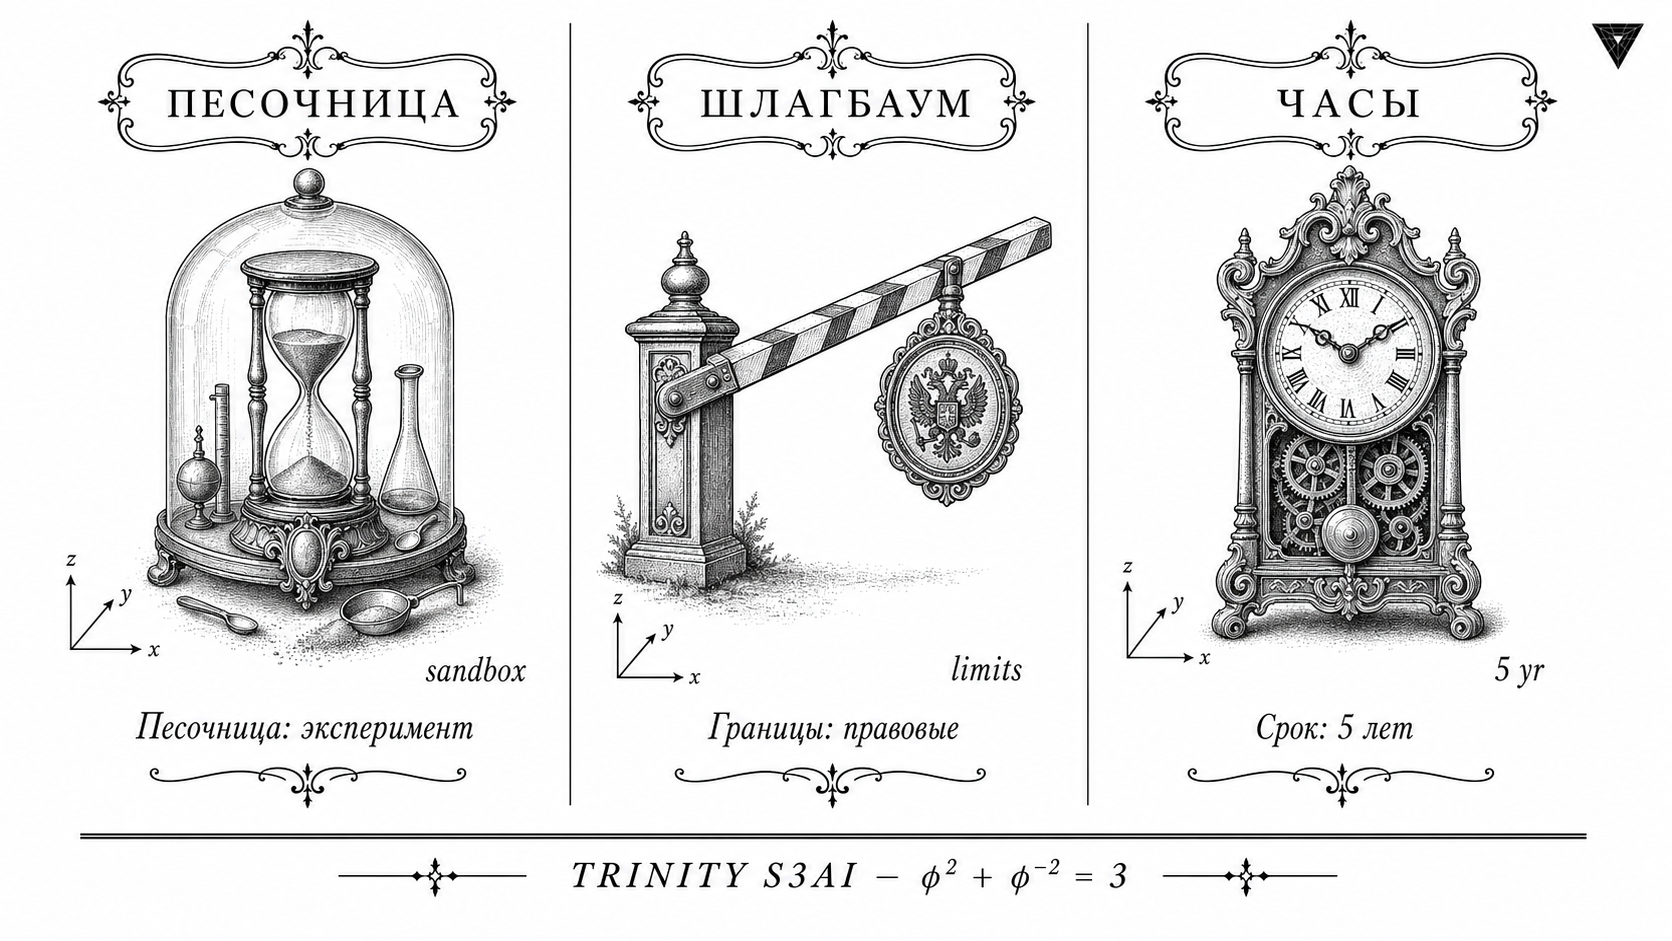
\includegraphics[keepaspectratio,alt={ЭПР --- песочница, границы, срок}]{figures/canon/r30_sec52_epr.png}}
\caption{ЭПР --- песочница, границы, срок}
\end{figure}

ФЗ № 258-ФЗ об ЭПР существенно обновлён: 10 июня 2026 г. Госдума приняла
закон о расширении применения ЭПР в интересах развития ИИ
(\href{https://www.interfax.ru/amp/1095191}{Интерфакс, 10.06.2026};
\href{https://d-russia.ru/prinyat-zakon-o-rasshirenii-primeneniya-epr-v-interesah-ii-razvitiya.html}{d-russia.ru}):
максимальный срок ЭПР увеличен до \textbf{5 лет}, требование о наличии
нормативного барьера как условия входа отменено, выход из режима --- по
мотивированному обращению самого участника. Это даёт Trinity
\textbf{конкретный механизм пилотирования} открытых троичных чипов в
реальных системах без ожидания вступления в силу закона об ИИ. Первичный
шаг --- обращение в Минцифры с описанием инновации.

\subsubsection{5.3. Рыночный спрос от
КИИ}\label{ux440ux44bux43dux43eux447ux43dux44bux439-ux441ux43fux440ux43eux441-ux43eux442-ux43aux438ux438}

Указ № 166 от 30.03.2022 требует перехода значимых объектов КИИ на
\textbf{доверенные программно-аппаратные комплексы к 01.01.2030}
(\href{http://www.kremlin.ru/acts/bank/47688}{kremlin.ru}). Это уже
закреплённый нормой спрос на проверяемые отечественные компоненты ---
рыночное обоснование тезиса «проверяемость», а не прогноз.

\subsubsection{5.4. Юрисдикция и суверенность: честно об открытом
вопросе}\label{ux44eux440ux438ux441ux434ux438ux43aux446ux438ux44f-ux438-ux441ux443ux432ux435ux440ux435ux43dux43dux43eux441ux442ux44c-ux447ux435ux441ux442ux43dux43e-ux43eux431-ux43eux442ux43aux440ux44bux442ux43eux43c-ux432ux43eux43fux440ux43eux441ux435}

\begin{quote}
\textbf{Открытый вопрос (без замалчивания).} Одна из рассматриваемых
коммерческих структур предполагает размещение прав на ИП в зарубежном
холдинге с последующим лицензированием российским партнёрам --- чтобы
сохранить международные опции (зарубежные инвесторы, зарубежные
гранты). Это в прямом \textbf{напряжении} с риторикой «всё отечественное
для реестра РФ». Честная позиция: \textbf{проверяемость обеспечивается
открытыми публикуемыми спецификациями независимо от юрисдикции владельца
IP}, а национальная приписка решается отдельным юридическим контуром
(российское ООО-лицензиат + регистрация РИД в РФ). Это осознанный и
\textbf{неокончательный} выбор \textbf{{[}открытая гипотеза{]}}, а не
решённый факт. \textbf{Конкретное ограничение, которое нужно учесть
заранее:} включение ПО в реестр отечественного (Постановление
Правительства № 1236 от 16.11.2015, ред.) требует, чтобы
правообладателем было российское юрлицо/ИП, а \textbf{доля прямого или
косвенного иностранного участия не превышала 49 \%}, при российском
единоличном исполнительном органе
(\href{https://terabit.ai/research/edinyj-reestr-rossijskogo-po-polnoe-rukovodstvo-po-registracii-i-meram-gospodderzhki}{разбор
требований реестра, 2026}). Поэтому зарубежный IP-холдинг и реестр РФ
совместимы только через российское ООО-лицензиат с контрольной
российской долей --- это сужает пространство решений и должно быть
зафиксировано в корпоративной структуре с самого начала
\textbf{{[}доказано --- норма; открытая гипотеза --- итоговая
структура{]}}.
\end{quote}

\textbf{Экспортный контроль и возможное будущее изготовление за рубежом ---
отдельная честная напряжённость.} Изготовление чипа за рубежом сейчас
\textbf{не планируется} (текущий уровень --- RTL/GDS-дизайн + FPGA-верификация
на AX7203); гипотетическая в будущем передача прав зарубежному IP-холдингу или
изготовление за рубежом являются, по смыслу
\textbf{ФЗ № 183-ФЗ «Об экспортном контроле»} и списка товаров и
технологий двойного назначения (\textbf{Постановление Правительства №
1299/2022},
\href{http://government.ru/docs/all/152564/}{government.ru}),
потенциальной \textbf{передачей (экспортом) технологии} и рассматривается
только как \textbf{{[}замысел/будущая опция{]}}. Общее правило: открытая
публикация RTL переводит её в \textbf{публичный домен} и, как правило,
выводит из-под экспортного контроля --- \textbf{кроме категории 5
(криптография)}. Поэтому: (а) при гипотетической передаче технологии за рубеж
в будущем российскому автору следует провести \textbf{идентификацию} на
принадлежность к списку ТДН; (б) криптографические узлы (см. § 5.7)
требуют отдельного внимания. Мы фиксируем это как \textbf{{[}открытая
гипотеза/проекция{]}}: точная квалификация зависела бы от состава RTL и
площадки гипотетического изготовления. \textbf{Зеркальная (иностранная) сторона
(гипотетическая).} При гипотетическом изготовлении за рубежом симметрично
действовал бы экспортный контроль \emph{страны изготовления}:
передовые полупроводниковые технологии и
САПР подпадают под ограничения, и доступ к ним для российского участника
может быть ограничен независимо от российских норм. Здесь открытость
работает в обе стороны: публикация дизайна как \emph{открытой научной
информации} и потенциальное изготовление на \emph{нечувствительных техпроцессах}
(зрелые узлы 65--250 нм) --- это путь, который не упирается в
передовую литографию и снижает санкционную уязвимость. Это согласуется с
самим тезисом «Россия 3.0»: доверенность строится на доступных, а не на
передовых узлах \textbf{{[}открытая гипотеза/проекция --- гипотетический
сценарий, не текущий маршрут{]}}.

\begin{center}\rule{0.5\linewidth}{0.5pt}\end{center}

\subsubsection{5.5. Авторство ИИ-кода: охрана при творческом вкладе
человека}\label{ux430ux432ux442ux43eux440ux441ux442ux432ux43e-ux438ux438-ux43aux43eux434ux430-ux43eux445ux440ux430ux43dux430-ux43fux440ux438-ux442ux432ux43eux440ux447ux435ux441ux43aux43eux43c-ux432ux43aux43bux430ux434ux435-ux447ux435ux43bux43eux432ux435ux43aux430}

Значительная часть кода Trinity (компилятор TRI-27, RTL чипов) создаётся
с частичной ИИ-помощью. По российскому праву (\textbf{ст. 1228, 1257,
1259 ГК РФ} и \textbf{Постановление Пленума Верховного Суда РФ № 10 от
23.04.2019, п. 80}, \href{https://base.garant.ru/58074501/}{garant.ru})
объектом авторского права признаётся результат, созданный
\textbf{творческим трудом человека}; «чисто машинный» результат охраны
не получает. Судебная практика 2024--2026 гг. (например, дела №
А40-200471/2023 и № А53-7527/2025) подтверждает: охрана возникает при
доказуемом творческом вкладе. \textbf{Практический вывод для Trinity:}
код с ИИ-ассистированием охраняется как РИД при условии
\textbf{документирования человеческого вклада} --- архитектурных
решений, ревью, правок. Рекомендуется вести журнал авторских решений как
доказательную базу. Это усиливает, а не ослабляет позицию автора
\textbf{{[}доказано --- нормы и практика; открытая гипотеза --- оценка
конкретного вклада судом{]}}.

\subsubsection{5.6. Патент на способ и устройство (дополнительно к
авторскому
праву)}\label{ux43fux430ux442ux435ux43dux442-ux43dux430-ux441ux43fux43eux441ux43eux431-ux438-ux443ux441ux442ux440ux43eux439ux441ux442ux432ux43e-ux434ux43eux43fux43eux43bux43dux438ux442ux435ux43bux44cux43dux43e-ux43a-ux430ux432ux442ux43eux440ux441ux43aux43eux43cux443-ux43fux440ux430ux432ux443}

Авторское право защищает форму выражения кода, но \textbf{не
идею/способ}. Поэтому ключевой недооценённый контур --- \textbf{патент}
(\textbf{ст. 1350 ГК РФ}; \textbf{Приказ Минэкономразвития № 148 от
15.03.2024} о требованиях к заявке; пошлины по \textbf{Постановлению
Правительства № 1278},
\href{https://rospatent.gov.ru/ru/activities/dues/table}{rospatent.gov.ru}).
GoldenFloat патентоспособен как \textbf{«способ вычисления в
тернарной/золотосечённой арифметике»} при доказанном техническом
результате; чип TRI-27 --- как \textbf{устройство}. Физлицо/самозанятый
пользуется \textbf{пониженными (льготными) пошлинами}; важно понимать,
что патентные пошлины --- \textbf{поэтапные}, а не один платёж: (1)
подача заявки и формальная экспертиза → (2) экспертиза по существу → (3)
регистрация и выдача патента, плюс ежегодные пошлины за поддержание
(\textbf{ст. 333.30 НК РФ; Постановление Правительства № 1278}
{[}действующая норма{]}). Конкретные суммы зависят от стадии и числа
пунктов формулы; единого «итогового» платежа не существует.
\textbf{Важно (снимает мнимое противоречие «открытый код против
патента»):} лицензия \textbf{Apache 2.0 содержит явную патентную
лицензию (patent grant)}, поэтому открытая публикация под Apache
\textbf{не означает автоматического отказа} от патентных прав на
способ/устройство --- открытость и патентование совместимы
\textbf{{[}доказано --- патентоспособность как право; открытая гипотеза
--- прохождение экспертизы на новизну{]}}.

\subsubsection{5.7. Криптофункция BLAKE3: квалификация по режиму
использования}\label{ux43aux440ux438ux43fux442ux43eux444ux443ux43dux43aux446ux438ux44f-blake3-ux43aux432ux430ux43bux438ux444ux438ux43aux430ux446ux438ux44f-ux43fux43e-ux440ux435ux436ux438ux43cux443-ux438ux441ux43fux43eux43bux44cux437ux43eux432ux430ux43dux438ux44f}

RTL-дизайн tt-trinity-euler использует криптографический якорь \textbf{BLAKE3}.
Квалификация зависит от \textbf{режима}: хеш-функция \textbf{без ключа}
(обычный BLAKE3) --- вероятно \textbf{не является СКЗИ};
\textbf{keyed-режим / MAC} (имитозащита) --- формально \textbf{СКЗИ}. По
\textbf{Постановлению Правительства № 313 от 16.04.2012}
(\href{https://base.garant.ru/70164728/}{garant.ru})
разработка/распространение СКЗИ лицензируется ФСБ; при
\textbf{распространении} средства с keyed-режимом требуется
\textbf{нотификация ЕЭК} (Решение Коллегии ЕЭК № 30, Приложение 9). При
использовании \textbf{для собственных нужд} лицензия не требуется.
\textbf{Практический вывод:} для открытой публикации и потенциального будущего
изготовления безопаснее опираться на \textbf{бесключевой} режим BLAKE3
(целостность/«печати» воспроизводимости), а keyed-режим (имитозащита)
выделять в отдельный контур с экспертизой ФСБ и нотификацией ЕЭК
\textbf{{[}открытая гипотеза --- квалификация режима; доказано --- сами
нормы{]}}.

\begin{center}\rule{0.5\linewidth}{0.5pt}\end{center}

\subsection{6. Матрица соответствия: цели государства ↔ компоненты
Trinity}\label{ux43cux430ux442ux440ux438ux446ux430-ux441ux43eux43eux442ux432ux435ux442ux441ux442ux432ux438ux44f-ux446ux435ux43bux438-ux433ux43eux441ux443ux434ux430ux440ux441ux442ux432ux430-ux43aux43eux43cux43fux43eux43dux435ux43dux442ux44b-trinity}

\begin{figure}
\centering
\pandocbounded{
\includegraphics[keepaspectratio,alt={Триптих фиг. 6 --- Цели НСРИИ ↔ компоненты Trinity ↔ регистрируемые РИД.}]{figures/canon/r30_sec6_matrix.png}}
\caption{Триптих фиг. 6 --- Цели НСРИИ ↔ компоненты Trinity ↔
регистрируемые РИД.}
\end{figure}

Ниже --- прямое сопоставление действующих государственных целей и того,
какой компонент стека их поддерживает. Это ядро согласованности
предложения.

{[}Таблица --- соответствие норма/цель ↔ компонент Trinity ↔ статус:{]}
- \textbf{Доверенный ИИ в ГИС --- действующее требование (Приказ ФСТЭК №
117, п. 61; ГОСТ Р 59276-2020)} ← GoldenFloat (воспроизводимая,
объяснимая арифметика) + оракул соответствия Corona + root-of-trust Phi
+ BLAKE3-проверка Euler. Статус: задел готов, верифицирован на FPGA;
норма уже действует. - \textbf{РИД: программа для ЭВМ --- ст. 1262 ГК РФ
(действует)} ← регистрация библиотеки GoldenFloat / компилятора TRI-27 /
VIBEE в Роспатенте. Статус: к подаче --- \textbf{доступно самозанятому
как физлицу}, 4 500 руб. - \textbf{РИД: топология ИМС --- ст. 1448--1464
ГК РФ (действует)} ← регистрация топологии RTL/GDS-дизайнов TRI-27 / tt-trinity.
Статус: к подаче --- \textbf{гражданин РФ как физлицо}, 5 000 руб.; срок
--- 2 года с первого раскрытия (срочно). - \textbf{Технологический
суверенитет (Распоряжение № 1315-р; ст. 1286.1 ГК)} ← открытый стек
TRI-27 с собственной линией разработки от спецификации до RTL; открытые
лицензии легальны по ст. 1286.1 ГК. Статус: открытый код,
Apache-2.0/MIT. - \textbf{Спрос КИИ на доверенные ПАК к 2030 (Указ №
166)} ← проверяемые отечественные компоненты (FPGA-дизайны + оракул
соответствия). Статус: рынок, закреплённый нормой. -
\textbf{Импортозамещение ПО / реестр (ПП № 1236)} ← регистрация
VIBEE/GoldenFloat в реестре отечественного ПО. Статус: формально
самозанятый подать может, но практически требуется ИП/ООО + ЭЦП. -
\textbf{Микроэлектроника на доступных топологиях (Распоряжение № 20-р,
28 нм)} ← верификация на FPGA (AX7203) без
потребности в 5 нм; RTL/GDS-дизайн как задел. Статус: FPGA --- измерено; изготовление
кремния не планируется. - \textbf{Доверие граждан к ИИ --- 80\% (НСРИИ)} ←
парадигма «проверяемость вместо TOPS»: техническая обоснованность
доверия. Статус: концептуально; требует пилота. - \textbf{Публикации
уровня A --- 450/год (НСРИИ)} ← публикационный трек (статьи в ВАК К-1,
препринты arXiv). Статус: 1-я статья в подаче в журнал
«Программирование». - \textbf{Кадры 15 500/год (НСРИИ)} ← открытый стек
как учебная платформа (троичность, числовые форматы, открытый RTL).
Статус: потенциал, требует партнёрства с вузами. - \textbf{Патент на
способ/устройство (ст. 1350 ГК; Приказ Минэк № 148/2024)} ← GoldenFloat
как «способ вычисления», RTL-дизайн TRI-27 как устройство; Apache 2.0 patent
grant совместим с патентом. Статус: к подаче доступно физлицу,
пониженные (льготные) пошлины; пошлины поэтапные (подача+формальная →
экспертиза по существу → регистрация/выдача + поддержание), ст. 333.30
НК РФ {[}действующая норма{]}; прохождение экспертизы --- открытая
гипотеза. - \textbf{Авторство ИИ-кода (ст. 1257, 1259 ГК; Пленум ВС № 10
п. 80)} ← охрана кода/RTL при доказанном творческом вкладе человека;
ведение журнала авторских решений. Статус: нормы и практика 2024--26 ---
доказано; оценка вклада --- гипотеза. - \textbf{Экспортный контроль (ФЗ
№ 183-ФЗ; ПП № 1299/2022)} ← открытая публикация RTL → публичный домен
(кроме категории 5/крипто); зарубежное изготовление = экспорт технологии
→ требуется идентификация. Статус: открытая напряжённость/проекция. -
\textbf{Доверенное ПО и ПАК (ПП № 1931 с 01.03.2026; ПП № 1912)} ←
компилятор/ПО --- трек «доверенного ПО»; чип --- доверенный ПАК для КИИ.
Статус: действующие/вступающие нормы; путь через тестирование и
Правкомиссию. - \textbf{Криптофункции / СКЗИ (ПП № 313; Решение ЕЭК №
30)} ← BLAKE3: бесключевой ≠ СКЗИ; keyed/MAC = СКЗИ (нотификация ЕЭК,
экспертиза ФСБ). Статус: квалификация по режиму --- гипотеза; нормы ---
доказано. - \textbf{Стандартизация форматов (ФЗ № 162-ФЗ; ТК 164)} ←
путь GoldenFloat → ПНСТ (ГОСТ на форматы чисел в РФ отсутствует).
Статус: реалистично при поддержке отраслевых партнёров --- открытая
гипотеза.

\begin{center}\rule{0.5\linewidth}{0.5pt}\end{center}

\subsection{7. Дорожная карта «Россия 3.0» (реалистичные
стадии)}\label{ux434ux43eux440ux43eux436ux43dux430ux44f-ux43aux430ux440ux442ux430-ux440ux43eux441ux441ux438ux44f-3.0-ux440ux435ux430ux43bux438ux441ux442ux438ux447ux43dux44bux435-ux441ux442ux430ux434ux438ux438}

\begin{figure}
\centering
\pandocbounded{
\includegraphics[keepaspectratio,alt={Триптих фиг. 7 --- Реалистичные стадии 2026 → 2028 → 2030.}]{figures/canon/r30_sec7_roadmap.png}}
\caption{Триптих фиг. 7 --- Реалистичные стадии 2026 → 2028 → 2030.}
\end{figure}

Предложение не требует мегабюджетов на старте --- оно построено по
принципу «доказывай дёшево, масштабируй по результату».

\begin{enumerate}
\def\labelenumi{\arabic{enumi}.}
\tightlist
\item
  \textbf{Стадия 0 (2026, \textasciitilde готово):} опубликованный
  формат, FPGA-кодек, открытый каталог, первая ВАК-статья в подаче.
  \textbf{{[}выполнено / в процессе{]}}
\item
  \textbf{Стадия 1 (2026--2027):} немедленная регистрация РИД ---
  программы для ЭВМ (ст. 1262 ГК РФ) и топологии ИМС TRI-27 (ст.
  1448--1464 ГК РФ) в Роспатенте (доступно физлицу); \textbf{подача
  патентной заявки на способ вычисления GoldenFloat и устройство TRI-27
  (ст. 1350 ГК РФ, льготные пошлины физлица)}; начало ведения
  \textbf{журнала авторских решений} для доказательства творческого
  вклада в ИИ-код; \textbf{учреждение российского юрлица (ООО) с
  контрольной российской долей} --- это сделано на данной стадии
  сознательно рано, поскольку юрлицо является \emph{ключом} к
  финансированию: большинство федеральных грантовых механизмов (ФСИ,
  РФРИТ, РНФ) и включение ПО в реестр отечественного (ПП № 1236) требуют
  статус МСП либо принадлежности прав российскому юрлицу; расширение
  FPGA-верификации (больше форматов Tier-E на AX7203); пилот «доверенного» инференса на
  отечественной FPGA в рамках обновлённого ЭПР (258-ФЗ, ред. 10.06.2026
  --- срок до 5 лет).
\item
  \textbf{Стадия 2 (2027--2028):} через уже учреждённое юрлицо ---
  заявки в грантовые механизмы (Сколково «Микроэлектроника»,
  «Развитие-НТИ» Нейронет, субсидии Минпромторга по ЭКБ) и включение в
  реестр отечественного ПО (ПП № 1236); инициирование \textbf{ПНСТ по
  формату GoldenFloat через ТК 164} при поддержке отраслевых партнёров;
  перенос reference-архитектур на отечественные чипы (доступные
  топологии); сертификационный трек ФСТЭК и трек \textbf{признания ПО
  доверенным (ПП № 1931)}; вхождение в реестр доверенных моделей ИИ (по
  мере вступления в силу регулирования 2027 г.; в редакции законопроекта
  2026 г. для статуса «национальной»/«суверенной» модели достаточно
  российского юрлица --- требование «только граждане РФ» снято,
  \href{https://pravo.ru/story/263957/}{ПРАВО.ru, дайджест за май 2026})
  \textbf{{[}законопроект, не действующая норма{]}}.
\item
  \textbf{Стадия 3 (2028--2030):} масштабирование как доверенного
  edge-стека (умные устройства, автономные системы, КИИ) в рамках НПТЛ;
  учебная платформа для подготовки кадров.
\end{enumerate}

\begin{quote}
\textbf{Устойчивость проекта (честно).} На июнь 2026 г. ядро разработки
держится на одном авторе --- это объективный риск устойчивости (bus
factor), и мы не маскируем его, а показываем конкретный план снижения.
\textbf{Что уже сделано как основа для команды:} (1) весь стек
опубликован под открытой лицензией (Apache-2.0/MIT) --- это снимает
зависимость от одного человека: код, спецификации и битоточные векторы
соответствия доступны и воспроизводимы любым участником; (2)
подготовлена первая научная публикация (в подаче в журнал
«Программирование») --- формальная точка входа для соавторов; (3)
международный гуманитарно-научный контур (проф. Скотт Олсен, Emeritus
Professor, College of Central Florida) уже привлечён к смежной работе о
математических основаниях формата. \textbf{Что планируется по стадиям:}
на Стадии 1 --- учреждение ООО как юридической оболочки для найма и
распределения прав; на Стадии 2 --- институционализация через
вуз/отраслевого партнёра и стандартизацию (ПНСТ через ТК 164), что
добавляет к проекту организацию, а не только человека. До получения
грантов проект развивается по принципу bootstrap --- за счёт открытого
кода и сервисов вокруг него, с последующим переходом к грантовому
финансированию через российское юрлицо и лицензированию РИД
\textbf{{[}доказано --- открытая лицензия и публикация; открытая
гипотеза --- состав будущей команды{]}}.
\end{quote}

\subsubsection{7.1. Ресурсы и отдача по
стадиям}\label{ux440ux435ux441ux443ux440ux441ux44b-ux438-ux43eux442ux434ux430ux447ux430-ux43fux43e-ux441ux442ux430ux434ux438ux44fux43c}

Чтобы предложение не выглядело «просьбой вообще», ниже --- честная
картина \emph{категорий} затрат и источников по стадиям. Конкретные
суммы намеренно не фиксируются: патентные и регистрационные пошлины
поэтапны и зависят от стадии и объёма (ст. 333.30 НК РФ), а грантовые
суммы определяются конкурсными условиями конкретной очереди.

{[}Таблица --- ресурсы и отдача по стадиям:{]}

\begin{itemize}
\tightlist
\item
  \textbf{Стадия 0--1 (2026--2027) --- задел и РИД.} Затраты: пошлины за
  регистрацию ПО и топологии ИМС (ст. 1262, 1448--1464 ГК РФ), поэтапные
  патентные пошлины (ст. 1350 ГК, льготы физлица), FPGA-плата
  (ALINX AX7203). \textbf{Источник:} личные
  средства исследователя (bootstrap). \textbf{Отдача:}
  зарегистрированные РИД как активы. \textbf{{[}план / частично
  выполнено{]}}
\item
  \textbf{Стадия 1 (2026--2027) --- юридическая оболочка.} Затраты:
  регистрация ООО, базовый бухучёт. \textbf{Источник:} личные средства.
  \textbf{Отдача:} ООО --- \emph{ключ} к грантам и реестру
  отечественного ПО. \textbf{{[}план{]}}
\item
  \textbf{Стадия 2 (2027--2028) --- грантовое финансирование НИОКР.}
  Затраты: НИОКР, перенос на отечественные чипы, сертификация.
  \textbf{Источник:} федеральные гранты через юрлицо (ФСИ
  СТАРТ-ИИ/Развитие-ИИ, Сколково, субсидии Минпромторга).
  \textbf{Отдача:} вхождение в реестры, ПНСТ, пилот для КИИ.
  \textbf{{[}план, зависит от открытия очередей{]}}
\item
  \textbf{Стадия 3 (2028--2030) --- масштабирование и выручка.} Затраты:
  продуктовые работы, поддержка. \textbf{Источник:} лицензирование РИД,
  госзакупки (приоритет отечественного ПО), сервисы. \textbf{Отдача:}
  доверенный edge-стек, кадры. \textbf{{[}открытая гипотеза /
  проекция{]}}
\end{itemize}

Принцип прост: \textbf{ранние стадии дёшевы и финансируются
самостоятельно, а государственная поддержка подключается только после
появления проверяемого результата и юрлица-получателя} --- это снижает
риск для бюджета.

\begin{center}\rule{0.5\linewidth}{0.5pt}\end{center}

\subsection{8. Открытое обращение к руководству
страны}\label{ux43eux442ux43aux440ux44bux442ux43eux435-ux43eux431ux440ux430ux449ux435ux43dux438ux435-ux43a-ux440ux443ux43aux43eux432ux43eux434ux441ux442ux432ux443-ux441ux442ux440ux430ux43dux44b}

\begin{figure}
\centering
\pandocbounded{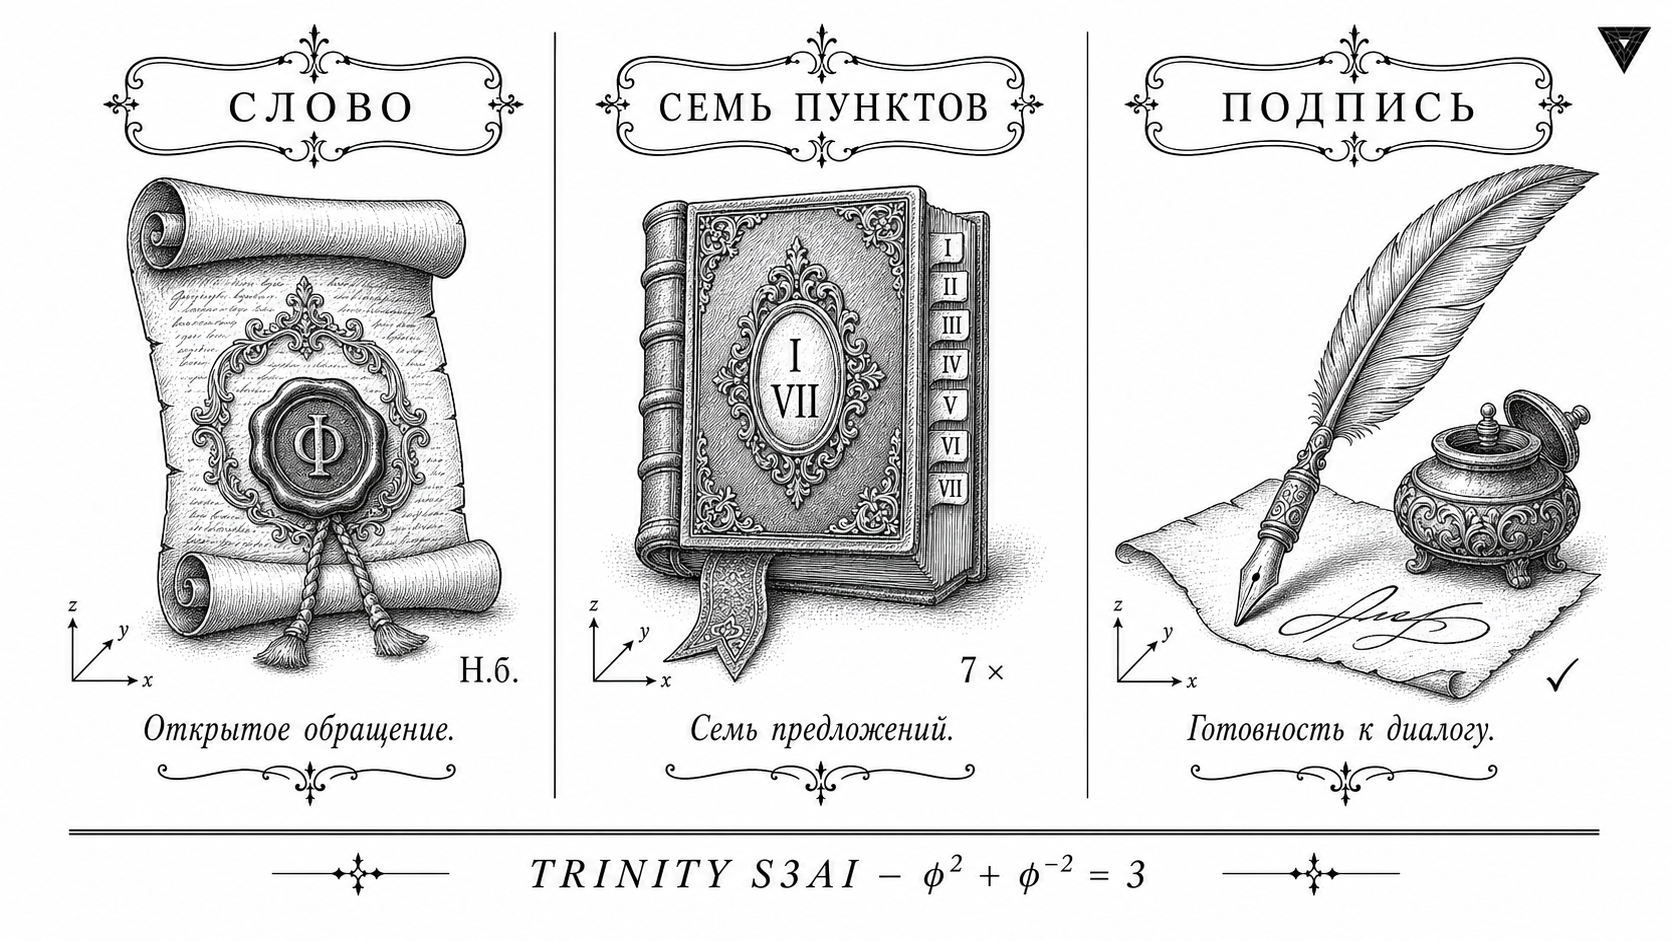
\includegraphics[keepaspectratio,alt={Триптих фиг. 8 --- Открытое обращение: слово, семь пунктов, готовность к диалогу.}]{figures/canon/r30_sec8_appeal.png}}
\caption{Триптих фиг. 8 --- Открытое обращение: слово, семь пунктов,
готовность к диалогу.}
\end{figure}

\emph{Настоящий раздел оформлен как открытое обращение в научном
формате. Он не претендует на нормативную силу и представляет собой
научно обоснованное предложение гражданина и исследователя.}

Уважаемый Президент Российской Федерации! Уважаемые члены Правительства
и научное сообщество!

Действующая Национальная стратегия развития ИИ (Указ № 490 в ред. Указа
№ 124) и Концепция технологического развития (№ 1315-р) верно определили
\textbf{доверенность и суверенность} как приоритеты. Я, как российский
исследователь, предлагаю практический, проверяемый и уже существующий
отечественный задел в этом направлении --- открытый вычислительный стек
Trinity S³AI --- и прошу рассмотреть семь конкретных мер.
\textbf{Встречная отдача государству} (чтобы предложение не было
односторонней просьбой): открытый стек под отечественной лицензией даёт
стране (1) неотчуждаемый отечественный РИД --- регистрируемые в
Роспатенте программы для ЭВМ и топологии ИМС; (2) национальный
технический ориентир --- формат-кандидат в ПНСТ при отсутствии ГОСТ на
форматы чисел; (3) учебную платформу для подготовки кадров (показатель
НСРИИ 15 500 выпускников/год); (4) проверяемый компонент доверенного ИИ
для ГИС и КИИ под уже действующее требование п. 61 Приказа ФСТЭК № 117.
То есть запрашиваемая поддержка возвращается государству конкретными
активами, а не тратится безвозвратно:

\begin{enumerate}
\def\labelenumi{\arabic{enumi}.}
\tightlist
\item
  \textbf{Включить «проверяемость вычислений» (verifiability) в систему
  КПЭ доверенного ИИ} наряду с производительностью --- как технически
  измеримое основание для целевого показателя доверия граждан 80\% и как
  практическую опору уже действующего требования п. 61 Приказа ФСТЭК №
  117 о доверенных технологиях ИИ в составе ГИС.
\item
  \textbf{Поддержать регистрацию топологий ИМС отечественных троичных
  чипов} (гл. 74 ГК РФ) и программ для ЭВМ (ст. 1262 ГК РФ) как
  доступный физлицу-исследователю путь закрепления РИД --- и упростить
  связку «открытая лицензия (ст. 1286.1 ГК) + регистрируемый РИД» для
  open-hardware-проектов.
\item
  \textbf{Предусмотреть для самозанятых исследователей и микрокоманд
  облегчённый вход в федеральные грантовые механизмы} (ФСИ, РФРИТ, РНФ),
  которые сегодня требуют статус МСП (ООО/ИП) --- поскольку именно такие
  команды создают ранний задел, не имея этого статуса.
\item
  \textbf{Создать пилот «доверенного инференса» на отечественной
  FPGA в рамках ЭПР} --- пользуясь обновлённым 258-ФЗ (принят
  10.06.2026: срок до 5 лет, без требования нормативного барьера) --- с
  открытой методикой воспроизводимости и оракулом соответствия форматам;
  и предусмотреть для таких пилотов трек вхождения в будущий реестр
  доверенных моделей ИИ.
\item
  \textbf{Связать публикационный и кадровый треки} (показатели НСРИИ 450
  публикаций и 15 500 выпускников в год) с открытыми учебными
  платформами на базе отечественного стека.
\item
  \textbf{Поддержать ускоренную стандартизацию отечественных числовых
  форматов через ТК 164} (ФЗ № 162-ФЗ): в РФ нет ГОСТ на форматы чисел
  --- целесообразно открыть путь предварительного национального
  стандарта (ПНСТ) для проверяемых форматов (включая GoldenFloat) как
  национального технического ориентира доверенных вычислений.
\item
  \textbf{Распространить патентную поддержку на open-hardware-проекты}
  --- учитывая, что лицензия Apache 2.0 содержит патентный grant и
  совместима с патентованием способа (ст. 1350 ГК РФ): субсидировать
  патентные пошлины и экспертизу для исследователей-физлиц,
  регистрирующих способы вычислений и устройства, чтобы открытость не
  оборачивалась потерей прав.
\end{enumerate}

Я не утверждаю, что Trinity --- единственный или лучший путь. Я
утверждаю проверяемое: это \textbf{работающий, опубликованный, открытый
отечественный задел}, прямо отвечающий заявленным государством
приоритетам доверенности и суверенитета. Готов предоставить полную
научно-техническую документацию и принять участие в экспертизе.

С уважением, Дмитрий Васильев, ORCID 0009-0008-4294-6159, научная группа
Trinity S³AI.

\begin{center}\rule{0.5\linewidth}{0.5pt}\end{center}

\subsection{8a. Глобальный слой доверенных устройств и общая экономика
доверия: от лампочки до электронного
ключа}\label{a.-ux433ux43bux43eux431ux430ux43bux44cux43dux44bux439-ux441ux43bux43eux439-ux434ux43eux432ux435ux440ux435ux43dux43dux44bux445-ux443ux441ux442ux440ux43eux439ux441ux442ux432-ux438-ux43eux431ux449ux430ux44f-ux44dux43aux43eux43dux43eux43cux438ux43aux430-ux434ux43eux432ux435ux440ux438ux44f-ux43eux442-ux43bux430ux43cux43fux43eux447ux43aux438-ux434ux43e-ux44dux43bux435ux43aux442ux440ux43eux43dux43dux43eux433ux43e-ux43aux43bux44eux447ux430}

\begin{figure}
\centering
\pandocbounded{
\includegraphics[keepaspectratio,alt={Триптих фиг. 8 --- От лампочки до электронного ключа: единый слой доверия.}]{figures/canon/r30_sec8a_global.png}}
\caption{Триптих фиг. 8 --- От лампочки до электронного ключа: единый
слой доверия.}
\end{figure}

\emph{Этот раздел --- научно оформленное расширение обращения от
национального задела к его международному экспортному потенциалу. Он
сохраняет ту же дисциплину честности: разделяет действующие нормы и
проекции, а «общую экономику» понимает как техническую
интероперабельность доверенных устройств, а не политическое
утверждение.}

\subsubsection{8a.1. Идея: общий язык доверия вместо общего поля
боя}\label{a.1.-ux438ux434ux435ux44f-ux43eux431ux449ux438ux439-ux44fux437ux44bux43a-ux434ux43eux432ux435ux440ux438ux44f-ux432ux43cux435ux441ux442ux43e-ux43eux431ux449ux435ux433ux43e-ux43fux43eux43bux44f-ux431ux43eux44f}

Мир раскалывается на технологические блоки, и каждый блок строит свои
закрытые стеки. Но у миллиардов людей есть общая, аполитичная
потребность: чтобы устройства вокруг них --- от лампочки в каждом доме
до электронного ключа от квартиры, автомобиля и компьютера --- были
\emph{проверяемыми}, а не «чёрными ящиками», которые можно тайно
выключить, взломать или превратить в инструмент давления. Доверие к
устройству --- не идеология, а общечеловеческий общий знаменатель.
Именно на этом уровне --- \emph{проверяемость вычисления и подлинность
устройства} --- возможна техническая кооперация даже между политически
разобщёнными юрисдикциями.

Предложение \textbf{«Россия 3.0»} работает именно на этом нижнем, общем
для всех уровне: \emph{доверенная арифметика и проверяемый корень
доверия устройства}. Именно поэтому российское ядро стека может стать не
барьером, а \emph{экспортируемым вкладом в мировую инфраструктуру
доверия} --- при условии, что он проходит международный комплаенс.

\subsubsection{8a.2. Российское ядро + глобальный экспорт: два контура
соответствия}\label{a.2.-ux440ux43eux441ux441ux438ux439ux441ux43aux43eux435-ux44fux434ux440ux43e-ux433ux43bux43eux431ux430ux43bux44cux43dux44bux439-ux44dux43aux441ux43fux43eux440ux442-ux434ux432ux430-ux43aux43eux43dux442ux443ux440ux430-ux441ux43eux43eux442ux432ux435ux442ux441ux442ux432ux438ux44f}

Стратегия строится по принципу \textbf{«российское ядро, глобальная
оболочка»}. Для российского рынка устройство и его прошивка
соответствуют действующим отечественным нормам (техническое
регулирование РФ и ЕАЭС); для экспорта то же устройство получает второй,
международный контур сертификации, не меняя ядро доверия. Технически это
возможно потому, что все современные рамки доверия к устройствам
опираются на одни и те же примитивы: аппаратный корень доверия,
сертификаты X.509, безопасную загрузку, подписанные обновления и
взаимную аутентификацию --- то есть на проверяемой арифметике и
криптографии, которые и есть ядро Trinity.

\textbf{Российский контур (действующие нормы).} Для IoT/умных устройств
в РФ действуют национальные стандарты протоколов (ГОСТ Р 71168-2023 ---
LoRaWAN, ГОСТ Р 70036-2022 --- NB-Fi, ГОСТ Р 59026-2024 --- NB-IoT) и ТК
194 «Кибер-физические системы» \textbf{{[}действующая норма{]}}
(\href{https://docs.cntd.ru/document/1304463285}{Техэксперт/Кодекс});
для обращения на рынке ЕАЭС электроника проходит обязательную оценку
соответствия по ТР ТС 020/2011 (знак EAC). Для объектов КИИ возможны
криптопреобразования по отечественным СКЗИ и требования п. 61 Приказа
ФСТЭК № 117 к доверенным технологиям ИИ (см. § 5) \textbf{{[}действующая
норма{]}}.

\textbf{Глобальный контур (рамки экспорта).} Для выхода на европейский,
американский и рынки Глобального Юга устройство должно пройти набор
международных рамок, которые к 2026--2027 гг. становятся обязательными.
Их нельзя трактовать как «чужие» --- это общий технический язык,
понимаемый везде:

{[}Таблица --- международные рамки доверенных устройств:{]}

\begin{longtable}[]{@{}
  >{\raggedright\arraybackslash}p{(\linewidth - 4\tabcolsep) * \real{0.3333}}
  >{\raggedright\arraybackslash}p{(\linewidth - 4\tabcolsep) * \real{0.3333}}
  >{\raggedright\arraybackslash}p{(\linewidth - 4\tabcolsep) * \real{0.3333}}@{}}
\toprule\noalign{}
\begin{minipage}[b]{\linewidth}\raggedright
Рамка
\end{minipage} & \begin{minipage}[b]{\linewidth}\raggedright
Что покрывает
\end{minipage} & \begin{minipage}[b]{\linewidth}\raggedright
Статус и сроки
\end{minipage} \\
\midrule\noalign{}
\endhead
\bottomrule\noalign{}
\endlastfoot
EU CRA (Cyber Resilience Act, Регл. 2024/2847) & Кибербезопасность всех
«цифровых» продуктов (вкл. умные замки, камеры, лампы) & Репортинг
уязвимостей с 11.09.2026; полное соотв. 11.12.2027
\textbf{{[}действующая норма{]}} \\
eIDAS 2.0 / EUDI Wallet (Регл. 2024/1183) & Цифровая личность и
электронные ключи гражданина & Кошельки всем гражданам ЕС к концу 2026;
приём рег. секторами с дек. 2027 \textbf{{[}действующая норма{]}} \\
Matter (Connectivity Standards Alliance) & Умный дом: royalty-free
стандарт, обязат. аттестация DAC (X.509) & Действует; сертификация через
CSA+ATL \textbf{{[}действующий стандарт{]}} \\
ISO/IEC 30141:2024 & Эталонная архитектура IoT, «trustworthiness by
design» & Действует; technology-neutral, secure boot, X.509, TLS 1.3
\textbf{{[}действующий стандарт{]}} \\
FIDO2 / WebAuthn (passkeys) & Беспарольный доступ, аппаратный ключ (NIST
AAL3) & \textgreater5 млрд passkeys (2026); удовлетворяет PSD2/PSD3
\textbf{{[}действующий стандарт{]}} \\
\end{longtable}

\emph{Источники:
\href{https://digital-strategy.ec.europa.eu/en/policies/cyber-resilience-act}{EU
CRA, Eur. Commission};
\href{https://digital-strategy.ec.europa.eu/en/policies/eudi-regulation}{eIDAS/EUDI
Wallet}; \href{https://csa-iot.org/all-solutions/matter/}{Matter,
CSA-IoT}; \href{https://www.iso.org/standard/88800.html}{ISO/IEC
30141:2024}; \href{https://fidoalliance.org/passkeys/}{FIDO Alliance,
passkeys}.}

Ключевое наблюдение: все эти рамки требуют одного и того же ---
\emph{проверяемого корня доверия и корректной криптографии}. Российские
ГОСТы и ЕАЭС-сертификация покрывают внутренний рынок; Matter, CRA,
ISO/IEC 30141 и FIDO2 --- экспортный. Ядро Trinity (проверяемые форматы
+ RTL-дизайн phi как корень доверия + euler с BLAKE3) технически совместимо с
обоими контурами \textbf{{[}открытая гипотеза{]}} (совместимость не
сертифицирована, это проектная цель, а не достигнутый факт).

\subsubsection{8a.3. От лампочки до электронного ключа: единый слой
доверия}\label{a.3.-ux43eux442-ux43bux430ux43cux43fux43eux447ux43aux438-ux434ux43e-ux44dux43bux435ux43aux442ux440ux43eux43dux43dux43eux433ux43e-ux43aux43bux44eux447ux430-ux435ux434ux438ux43dux44bux439-ux441ux43bux43eux439-ux434ux43eux432ux435ux440ux438ux44f}

Практически «общая экономика доверия» означает, что один и тот же
проверяемый примитив применим на всех уровнях «умного» мира:

\begin{itemize}
\tightlist
\item
  \textbf{Лампочка / бытовой датчик (массовый, дешёвый уровень).} Даже
  лампа в умном доме должна иметь подлинный идентификатор и подписанную
  прошивку, иначе она становится точкой входа в ботнет. Здесь работают
  Matter (DAC) и EU CRA; ядро Trinity даёт \emph{дешёвый проверяемый
  корень доверия} (RTL-дизайн phi на FPGA) без дорогой литографии --- это прямое
  следствие тезиса «проверяемость вместо TOPS» (§ 3) \textbf{{[}открытая
  гипотеза{]}}.
\item
  \textbf{Бытовой шлюз / роутер (средний уровень).} Собирает доверенные
  устройства в сеть с взаимной аутентификацией (ISO/IEC 30141, TLS 1.3).
  Здесь пересекается наша линия доверенных сетей (TRI-NET) и
  отечественных сетевых процессоров (НПЦ «Элвис», см. § 3b).
\item
  \textbf{Электронный ключ / цифровая личность (верхний, критичный
  уровень).} Ключ от квартиры, автомобиля, компьютера и банковского
  доступа. Здесь работают FIDO2/passkeys (аппаратно-связанный ключ, NIST
  AAL3) и eIDAS 2.0 (государственный кошелёк личности). Ядро Trinity
  (phi как аппаратный корень доверия + euler с BLAKE3 как функция
  безопасности) --- это ровно тот класс примитивов, который требуют эти
  рамки \textbf{{[}доказано --- по классу примитивов; открытая гипотеза
  --- по сертифицированной совместимости{]}}.
\end{itemize}

От дешёвой лампочки до критичного ключа --- это \emph{один непрерывный
слой доверия}, различающийся лишь уровнем гарантий, а не природой
примитива. Именно это делает возможной \emph{общую экономику доверенных
устройств}: производитель в любой стране может встроить один и тот же
проверяемый корень, а потребитель --- независимо проверить его, не
доверяя вендору на слово.

\subsubsection{8a.4. Роль России и «Троицы» в глобальном
контуре}\label{a.4.-ux440ux43eux43bux44c-ux440ux43eux441ux441ux438ux438-ux438-ux442ux440ux43eux438ux446ux44b-ux432-ux433ux43bux43eux431ux430ux43bux44cux43dux43eux43c-ux43aux43eux43dux442ux443ux440ux435}

Открытость стека (Apache-2.0, открытые биточные векторы, RTL) превращает
российское ядро в \emph{экспортопригодный общественный актив}, а не в
закрытый национальный секрет. Это снимает главный барьер экспорта
доверенных технологий --- \emph{непроверяемость}: любая сторона может
воспроизвести спецификацию, проверить референсные векторы и убедиться,
что в корне доверия нет закладки. Для Глобального Юга (БРИКС, ШОС,
Африка, Юго-Восточная Азия) это особенно ценно: страны, не имеющие
собственной передовой литографии, получают \emph{проверяемый фундамент
доверия, воспроизводимый на доступных технологиях} (FPGA, зрелые
топологии), без зависимости от закрытых чёрных ящиков любого блока.

Честная оговорка: этот раздел --- \emph{стратегическое видение}, а не
достигнутый результат. Trinity сегодня --- это опубликованные форматы и
FPGA-кодек (§ 4), а не сертифицированный по Matter/CRA продукт. Но
\emph{архитектурно} стек изначально спроектирован под те же примитивы,
что требуют эти рамки, и именно поэтому может стать российским вкладом в
мировую инфраструктуру доверия --- язык, на котором можно договариваться
даже там, где трудно договориться о другом.

\subsubsection{8a.5. Суверенная доверенная основа: позиционирование
относительно Bitcoin/PoW {[}открытая гипотеза / стратегическое
позиционирование{]}}\label{a.5.-ux441ux443ux432ux435ux440ux435ux43dux43dux430ux44f-ux434ux43eux432ux435ux440ux435ux43dux43dux430ux44f-ux43eux441ux43dux43eux432ux430-ux43fux43eux437ux438ux446ux438ux43eux43dux438ux440ux43eux432ux430ux43dux438ux435-ux43eux442ux43dux43eux441ux438ux442ux435ux43bux44cux43dux43e-bitcoinpow-ux43eux442ux43aux440ux44bux442ux430ux44f-ux433ux438ux43fux43eux442ux435ux437ux430-ux441ux442ux440ux430ux442ux435ux433ux438ux447ux435ux441ux43aux43eux435-ux43fux43eux437ux438ux446ux438ux43eux43dux438ux440ux43eux432ux430ux43dux438ux435}

\begin{figure}
\centering
\pandocbounded{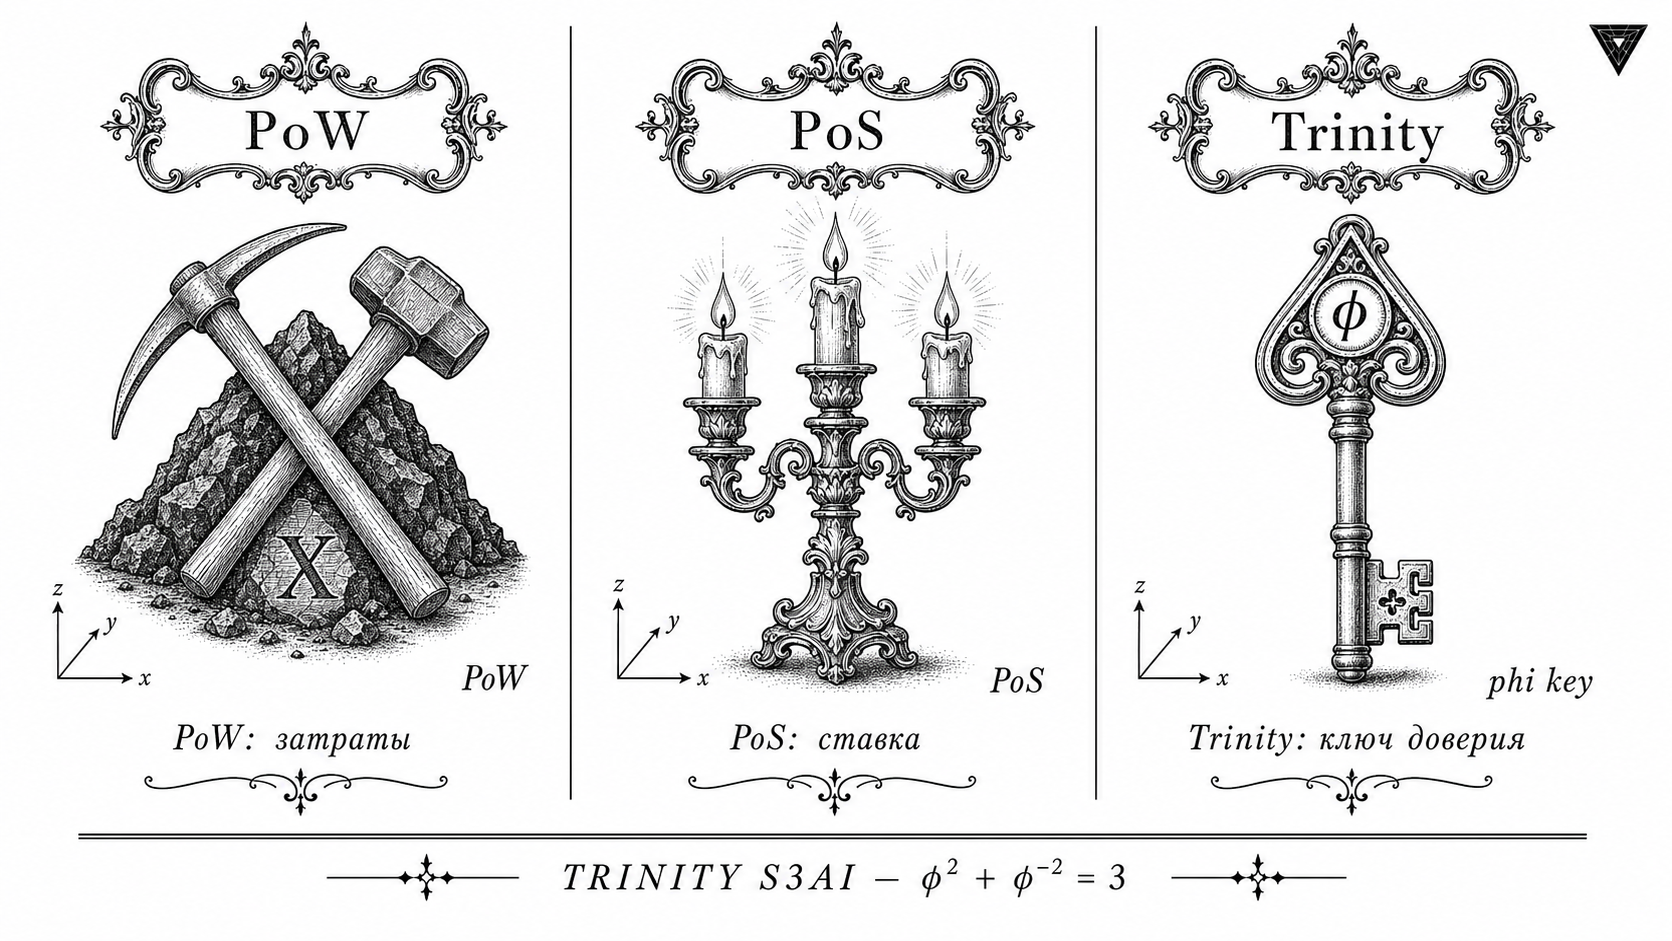
\includegraphics[keepaspectratio,alt={vs Bitcoin/PoW --- PoW, PoS, Trinity}]{figures/canon/r30_sec8a5_vs_pow.png}}
\caption{vs Bitcoin/PoW --- PoW, PoS, Trinity}
\end{figure}

Этот подраздел отвечает на естественный вопрос: \emph{как «Троица»
соотносится с Bitcoin и другими криптовалютами на блокчейне?} Ответ
требует аккуратного разграничения, чтобы не подменять понятия.

\textbf{Что Trinity НЕ является.} Trinity --- \emph{не} криптовалюта,
\emph{не} платёжная система и \emph{не} конкурент Bitcoin как денег. У
стека нет собственной монеты, эмиссии или механизма расчётов. Прямое
сравнение «Trinity против Bitcoin» как двух валют было бы некорректным
{[}методологическая оговорка{]}.

\textbf{В чём осмысленное сопоставление.} Сопоставимы не «деньги против
денег», а \emph{модели доверия}. Bitcoin предложил миру доверие
\emph{без доверенного посредника} --- за счёт публичного блокчейна и
доказательства работы (Proof-of-Work, PoW). Платой за это стали: (а)
внеюрисдикционность --- система принципиально не привязана к
национальному правовому полю; (б) высокое энергопотребление PoW ---
оценки годового потребления сети Bitcoin находятся в диапазоне
десятков-сотен ТВт·ч (\href{https://ccaf.io/cbnsi/cbeci}{Cambridge
CBECI};
\href{https://digiconomist.net/bitcoin-energy-consumption}{Digiconomist})
{[}измерено третьими сторонами, оценка{]}.

\textbf{Альтернативная модель «Троицы»: суверенная доверенная основа
(«золотая цепь»).} Trinity предлагает не замену деньгам, а
\emph{проверяемый фундамент доверия}, на котором суверенная цифровая
экономика \emph{может} быть построена. Три слоя этой основы: (1)
доверенный числовой слой --- GoldenFloat с бит-в-бит воспроизводимой
арифметикой (§ 4.1, 4a); (2) проверяемый корень доверия устройства ---
RTL-дизайны «Троица», верифицированные на FPGA, с открытым RTL и SHA-256-печатями соответствия; (3)
глобальный контур доверия --- TRI NET как сеть проверяемых устройств (§
8a). В отличие от PoW, доверие здесь обеспечивается
\emph{воспроизводимостью и открытой проверкой} (любая сторона
воспроизводит спецификацию и сверяет векторы), а не сжиганием энергии в
соревновании за блок {[}архитектурное свойство, не измерение{]}.

\textbf{Ключевые различия (сводно).}

\begin{longtable}[]{@{}
  >{\raggedright\arraybackslash}p{(\linewidth - 4\tabcolsep) * \real{0.3333}}
  >{\raggedright\arraybackslash}p{(\linewidth - 4\tabcolsep) * \real{0.3333}}
  >{\raggedright\arraybackslash}p{(\linewidth - 4\tabcolsep) * \real{0.3333}}@{}}
\toprule\noalign{}
\begin{minipage}[b]{\linewidth}\raggedright
Измерение
\end{minipage} & \begin{minipage}[b]{\linewidth}\raggedright
Bitcoin / PoW
\end{minipage} & \begin{minipage}[b]{\linewidth}\raggedright
Trinity / «золотая цепь» (TRI NET)
\end{minipage} \\
\midrule\noalign{}
\endhead
\bottomrule\noalign{}
\endlastfoot
Природа объекта & Децентрализованные деньги на блокчейне & Доверенная
вычислительная основа (не деньги) \\
Источник доверия & Доказательство работы (энергозатратное) &
Воспроизводимость + открытая проверка артефактов \\
Юрисдикция & Внеюрисдикционная по замыслу & Суверенная: совместима с
правовым полем РФ \\
Энергомодель & Высокое потребление PoW {[}измерено третьими{]} &
Проверяемая энергометрика (J/\text{op}) (§ 4a.3) {[}методология{]} \\
Что строится сверху & Расчёты, средство сбережения & Цифровая экономика
доверенных устройств и сервисов \\
\end{longtable}

\textbf{Честная граница тезиса.} Утверждение «Trinity --- суверенная
доверенная основа, альтернативная модели доверия Bitcoin» --- это
\emph{стратегическое позиционирование и открытая гипотеза} {[}открытая
гипотеза{]}, а не доказанный результат и не претензия на вытеснение
Bitcoin. Доказанная часть на сегодня --- это форматы, FPGA-кодек и
открытый код (§ 4). Тезис о «суверенной доверенной основе для цифровой
экономики» относится к видению развития, а не к достигнутому состоянию.

\begin{center}\rule{0.5\linewidth}{0.5pt}\end{center}

\subsubsection{8a.6. TRI NET как суверенный DePIN-контур: потенциальный
приток валюты в экономику РФ {[}открытая гипотеза /
проекция{]}}\label{a.6.-tri-net-ux43aux430ux43a-ux441ux443ux432ux435ux440ux435ux43dux43dux44bux439-depin-ux43aux43eux43dux442ux443ux440-ux43fux43eux442ux435ux43dux446ux438ux430ux43bux44cux43dux44bux439-ux43fux440ux438ux442ux43eux43a-ux432ux430ux43bux44eux442ux44b-ux432-ux44dux43aux43eux43dux43eux43cux438ux43aux443-ux440ux444-ux43eux442ux43aux440ux44bux442ux430ux44f-ux433ux438ux43fux43eux442ux435ux437ux430-ux43fux440ux43eux435ux43aux446ux438ux44f}

\begin{figure}
\centering
\pandocbounded{\includegraphics[keepaspectratio,alt={Триптих фиг. 9 --- TRI-NET как суверенный DePIN-контур {[}открытая гипотеза{]}.}]{figures/canon/r30_sec8a6_depin.png}}
\caption{Триптих фиг. 9 --- TRI-NET как суверенный DePIN-контур
{[}открытая гипотеза{]}.}
\end{figure}

Раздел § 8a.5 описал РОЛЬ «золотой цепи» как доверенной основы. Этот
подраздел отвечает на экономический вопрос: \emph{может ли сеть
проверяемых устройств TRI NET стать источником притока валюты в
российскую экономику?} Ответ формулируется строго как \textbf{открытая
гипотеза / проекция}, а не как обещание дохода.

\textbf{Что такое DePIN (контекст).} DePIN (Decentralized Physical
Infrastructure Networks) --- модель, при которой владельцы реального
оборудования (датчики, точки беспроводного доступа, вычислители,
хранилища) предоставляют инфраструктурные услуги и получают оплату. По
открытым оценкам третьих сторон, сектор охватывает порядка 40 млн
устройств в 199 странах с совокупной капитализацией порядка 9--10 млрд
долл. США (по данным на весну 2026 г.; пиковые оценки доходили до
\textasciitilde19 млрд долл.)
(\href{https://cryptoslate.com/cryptos/depin/}{CryptoSlate, DePIN};
\href{https://www.panewslab.com/zh/articles/019e5e0a-11b2-73d6-af9b-84b67a8c1123}{PANews})
{[}измерено третьими сторонами, оценка{]}. Реальная выручка от
некрипто-клиентов (реальный спрос на услуги) оценивалась в
\textgreater800 млн долл. в годовом выражении на I кв. 2026 г.
(\href{https://coinfomania.com/blockchain-news-2026-whats-actually-happening-right-now/}{Coinfomania})
{[}измерено третьими сторонами, оценка{]}.

\textbf{Гипотеза.} TRI NET --- это сеть из узлов с проверяемым корнем
доверия (§ 8a). Если такая сеть развёрнута как суверенный DePIN-контур с
отечественным ядром и глобальной оболочкой (§ 8a.2), то зарубежные
потребители инфраструктурных услуг (связь, вычисления, хранение, данные
датчиков) могут оплачивать их владельцам-операторам в РФ. В этой модели
возникает \emph{экспорт инфраструктурной услуги} --- приток валютной
выручки из-за рубежа, часть которой через налоги (НПД/НДС/налог на
прибыль) поступает в бюджет {[}открытая гипотеза / проекция{]}.

\textbf{Критическая правовая рамка (действующие нормы РФ 2026).} Эта
гипотеза обязана учитывать российское регулирование: с 01.07.2026
торговля криптовалютой легальна только через лицензированных
посредников; \emph{внутренние} расчёты криптовалютой в РФ запрещены
(рубль --- единственное законное платёжное средство); однако
\emph{трансграничные} расчёты российских компаний с иностранными
контрагентами разрешены
(\href{https://coinjuice.com/research-hub/russia-crypto-2026-bitcoin-ethereum-cbr}{CoinJuice,
Russia crypto 2026};
\href{https://companies.rbc.ru/amp/news/315deb89-e850-4bed-b74a-e50e30731e74/}{РБК})
{[}действующая норма с 01.07.2026{]}. Это означает: модель «приток
валюты в казну» допустима именно как \emph{экспорт услуги за рубеж}
(трансграничная выручка), а не как внутренняя крипто-расчётная система.
Любая реализация должна быть выстроена строго в этом правовом поле.

\textbf{Честная граница тезиса.} На июнь 2026 г. TRI NET не является ни
развёрнутой DePIN-сетью, ни источником дохода; RTL-дизайны «Троица» верифицированы
на FPGA, сеть не построена. Цифры DePIN-рынка относятся к
\emph{сектору в целом}, а не к Trinity. Оценка потенциальной доли или
притока в казну не проводилась и не моделировалась. Тезис «TRI NET как
суверенный DePIN-контур, приводящий валюту в экономику РФ» --- это
\emph{стратегическая проекция} {[}открытая гипотеза / проекция{]},
которая опирается на (а) реальный размер мирового DePIN-рынка как
ориентир и (б) действующее разрешение трансграничных расчётов. Для
проверки/опровержения гипотезы нужны: пилот развёртывания узлов, модель
спроса на услуги из-за рубежа и юридическая схема расчётов через
лицензированных посредников.

\subsubsection{8a.7. Токен \$TRI как ЦФА: легальный финансовый
инструмент для «Троицы» в правовом поле РФ {[}рабочее
предложение{]}}\label{a.7.-ux442ux43eux43aux435ux43d-tri-ux43aux430ux43a-ux446ux444ux430-ux43bux435ux433ux430ux43bux44cux43dux44bux439-ux444ux438ux43dux430ux43dux441ux43eux432ux44bux439-ux438ux43dux441ux442ux440ux443ux43cux435ux43dux442-ux434ux43bux44f-ux442ux440ux43eux438ux446ux44b-ux432-ux43fux440ux430ux432ux43eux432ux43eux43c-ux43fux43eux43bux435-ux440ux444-ux440ux430ux431ux43eux447ux435ux435-ux43fux440ux435ux434ux43bux43eux436ux435ux43dux438ux435}

\begin{figure}
\centering
\pandocbounded{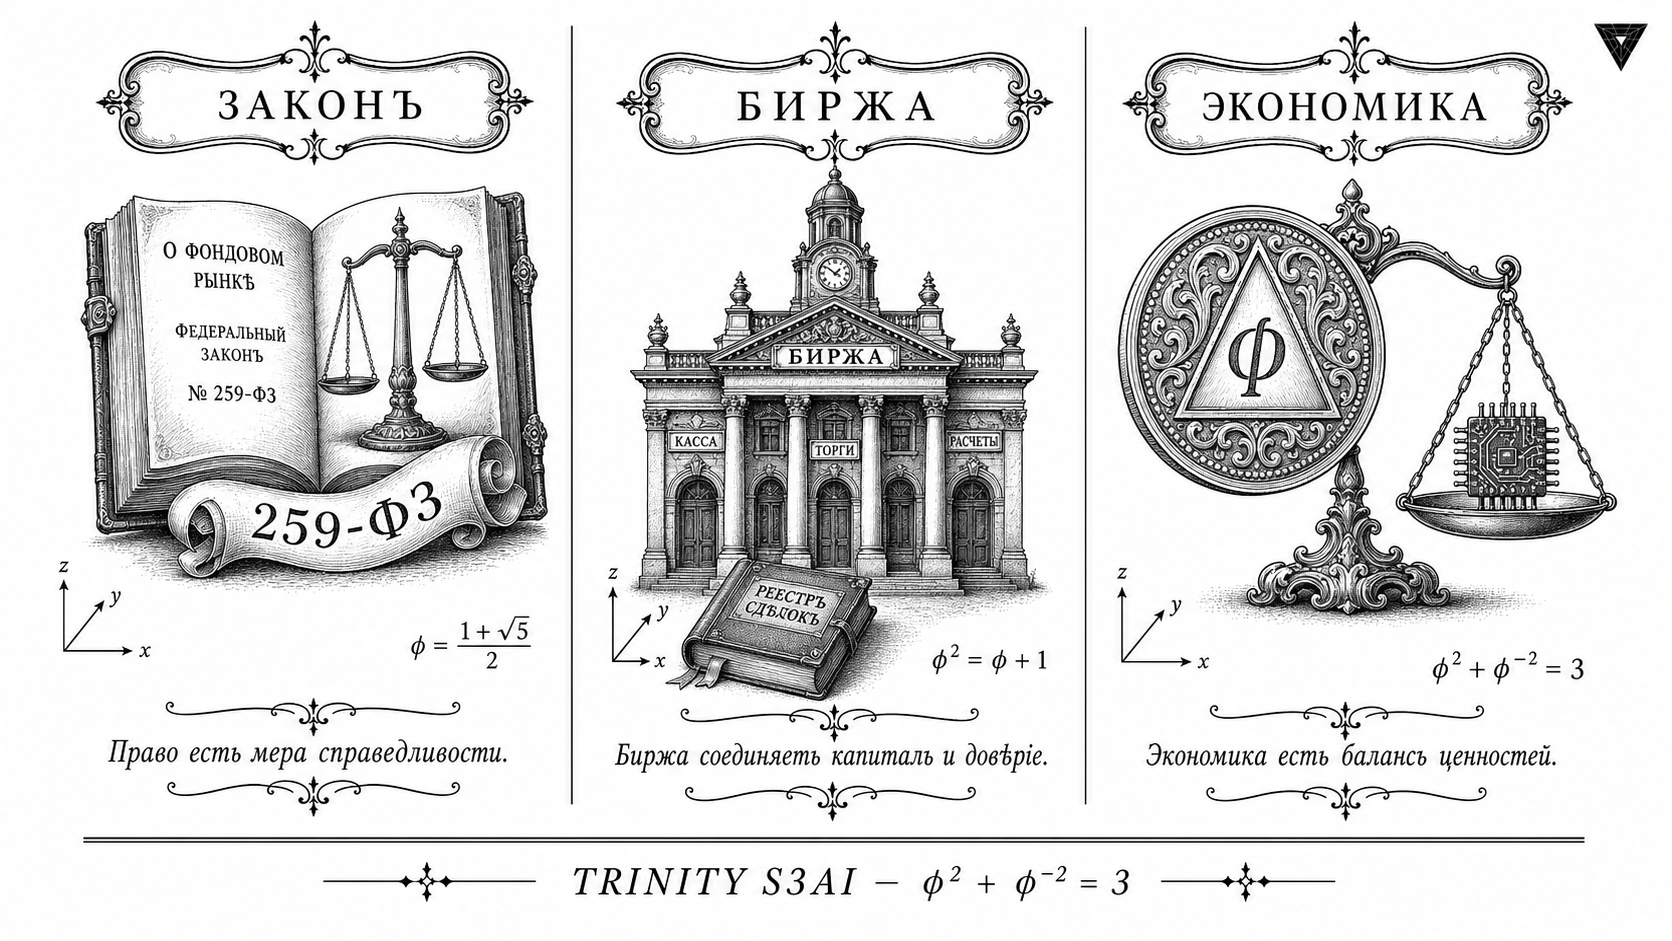
\includegraphics[keepaspectratio,alt={Триптих фиг. 8a.7 --- \$TRI как ЦФА: 259-ФЗ, оператор, гибридное цифровое право.}]{figures/canon/r30_sec8a7_tri_cfa.png}}
\caption{Триптих фиг. 8a.7 --- \$TRI как ЦФА: 259-ФЗ, оператор,
гибридное цифровое право.}
\end{figure}

Предыдущие подразделы описали \emph{техническую} основу (GoldenFloat +
RTL-дизайны «Троица» + TRI NET). Этот подраздел отвечает на финансовый вопрос:
\emph{как привлечь капитал в проект «Троицы» в действующем правовом поле
РФ, без оффшорных схем и без выпуска криптовалюты внутри страны?} Ответ
--- \textbf{через выпуск токена \$TRI как цифрового финансового актива
(ЦФА) в одной из лицензированных Банком России информационных систем}.

\textbf{Зачем именно ЦФА, а не криптовалюта или акции.} С 1 июля 2026 г.
в РФ действует обновлённая архитектура цифровых расчётов: внутренние
расчёты криптовалютой запрещены, использование криптовалют разрешено
только во внешнеторговых контрактах через лицензированных посредников;
одновременно ФНС требует обязательное уведомление о зарубежных
крипто-операциях
(\href{https://akft.ru/novosti/otkrytyj-vecher-akademii-glavnye-izmeneniya-rynka-czfa-s-1-iyulya-2026-goda/}{Академия
КФТ --- изменения с 01.07.2026}) {[}действующая норма{]}. Это означает:
токен «Троицы», выпущенный как «криптовалюта», окажется в крайне узком
правовом коридоре. \textbf{ЦФА --- наоборот, прямо разрешённый
внутренний инструмент}, обращающийся через 21 оператора информационных
систем (ОИС) в реестре ЦБ (\href{https://cbonds.ru/dfa/}{Cbonds, DFA};
\href{https://procfa.ru/reestr-platform-czfa-popolnilsya-novoj-kompaniej/}{Procfa})
{[}действующая норма{]}.

\textbf{Состояние рынка ЦФА (I кв. 2026, факты ЦБ РФ).} По данным Банка
России: суммарная стоимость действующих выпусков ЦФА --- \textbf{1,375
трлн руб.} (рост в 4,5 раза за 12 месяцев); первичные размещения за
квартал --- \textbf{1,135 трлн руб.} (≈69\% всего объёма 2025 года);
количество выпусков --- 1 512; зарегистрированных пользователей платформ
--- 910 982
(\href{https://abn.agency/2026/06/11/rynok-czfa-prevysil-1375-trln-rublej/}{Агентство
Бизнес Новостей};
\href{https://tenchat.ru/media/5504853-1375-trln-rubley-za-kvartal-rynok-tsfa-udvoilsya-i-prodolzhayet-rasti}{TenChat})
{[}измерено ЦБ РФ{]}. Прогноз ПСБ --- 3 трлн руб. за весь 2026 г.;
оценка Минфина --- \textbf{до 10 трлн руб. к 2030 г.}
(\href{https://rg.ru/amp/2026/05/18/vecherom-dengi.html}{Российская
газета}) {[}прогноз{]}. Юридические лица обеспечивают 93,9\% денежного
оборота --- рынок остаётся \textbf{корпоративным}, что прямо подходит
модели «Троицы»: эмиссия для институциональных инвесторов, не для
розницы.

\textbf{Меморандум ЦИПР 19.05.2026 --- прямой контекст для \$TRI.} На
конференции «Цифровая индустрия промышленной России» в Нижнем Новгороде
Сбер, Ассоциация крупнейших потребителей программного обеспечения и
оборудования (АКПО), «Ростелеком», ВТБ и «РЖД-Технологии» подписали
\textbf{меморандум о развитии ЦФА как инструмента для проектов в сфере
технологической независимости}
(\href{https://lenta.ru/news/2026/05/19/na-tsipr-podpisan-memorandum-o-tsfa-dlya-proektov-v-sfere-tehnologicheskoy-nezavisimosti/}{Lenta.ru,
19.05.2026}) {[}меморандум, не закон{]}. Цитата Виталия Трепыхалина
(«Ростелеком»): «Интеграция цифровых финансовых активов в рамках
проектов технологической независимости --- это шаг к формированию новой
цифровой инфраструктуры, обеспечивающей суверенитет нашей страны».
\textbf{Проект «Троицы» --- прямой кандидат на пилотное применение этой
рамки}: открытое отечественное железо + проверяемая арифметика + цепочка
от CPU-эмуляции до FPGA (AX7203) --- именно тот класс «сложных продуктовых
конструкций и консорциумов», под который писался меморандум.

\textbf{Прецедент Группы Астра (8 июня 2026) --- ближайший аналог
\$TRI.} ПАО «Группа Астра» провела \textbf{дебютный выпуск гибридных
цифровых прав (ГЦП)} на программно-аппаратный комплекс Astra XConnect
К100 на платформе «Токеон» (ПСБ); сбор заявок 8--22 июня 2026 г.,
максимальный объём --- 10 шт.; держатели ГЦП могут с 14 сентября по 7
октября 2026 г. либо получить ПАК физически, либо денежную выплату при
погашении 21 октября 2026 г.
(\href{https://www.cnews.ru/news/line/2026-06-05_gruppa_astra_obyavlyaet}{CNews};
\href{https://www.vedomosti.ru/investments/articles/2026/06/04/1202800-gruppa-astra-debyutiruet-na-rinke-gibridnih-tsifrovih-prav}{Ведомости};
\href{https://habr.com/ru/companies/astralinux/articles/1043876/}{Habr/Astra
Linux}) {[}действующий выпуск{]}. Это \textbf{доказательство, что ГЦП на
отечественный ПАК --- рабочая схема в правовом поле РФ}. Для \$TRI на
«Троицу» эта механика воспроизводится один-к-одному: эмитент ---
оператор «Троицы»; базовый актив --- модуль/плата на чипе «Троица»
(после возврата с фабрики); двойное право держателя --- получить чип
физически или денежную выплату.

\textbf{Какой именно тип цифрового права подходит \$TRI.} По 259-ФЗ
существует четыре подтипа ЦФА (денежное требование, право участия в
капитале, право по эмиссионным ЦБ, право требовать передачи ЦБ) и две
смежные конструкции --- утилитарные цифровые права (УЦП) и
\textbf{гибридные цифровые права (ГЦП)}
(\href{https://alfabank.ru/alfa-investor/posts/t/36b3a704-3866-f111-91c6-0050569e1fd0/}{Альфа-Банк,
классификация ЦФА};
\href{https://toveks.ru/\%F0\%9F\%94\%B4-normativnye-trebovaniya-i-regulyatornye-riski-blokchejn-proektov/}{259-ФЗ}).
Под архитектуру «Троицы» лучше всего ложатся два варианта:

\begin{itemize}
\tightlist
\item
  \textbf{Базовая конструкция --- долговой ЦФА «\$TRI-D» (денежное
  требование).} Краткосрочное (6--18 мес.) фондирование под
  фиксированную ставку, аналог квази-облигации; доминирует на рынке
  (более 80\% выпусков). Преимущество: понятная регуляторам и инвесторам
  конструкция, простая модель погашения, нет привязки к технической
  готовности железа. Подходит для финансирования следующего этапа
  разработки RTL/верификации.
\item
  \textbf{Расширенная конструкция --- гибридное цифровое право «\$TRI-H»
  (ГЦП).} По модели Группы Астра: базовый актив --- модуль на чипе
  «Троица»; держатель в окне погашения выбирает между физической
  поставкой модуля и денежной выплатой. Преимущество: токен напрямую
  связан с производимым продуктом (а не с долгом); вход для
  институционалов, готовых забрать железо; механика «капитал → железо»,
  а не «капитал → процент».
\end{itemize}

\textbf{Платформы-кандидаты для эмиссии \$TRI (с обоснованием).} Реестр
ЦБ на июнь 2026 г. насчитывает 21 ОИС; для проекта «Троицы» релевантны
платформы с опытом B2B-выпусков под IT/импортозамещение:

\begin{longtable}[]{@{}
  >{\raggedright\arraybackslash}p{(\linewidth - 6\tabcolsep) * \real{0.2500}}
  >{\raggedright\arraybackslash}p{(\linewidth - 6\tabcolsep) * \real{0.2500}}
  >{\raggedright\arraybackslash}p{(\linewidth - 6\tabcolsep) * \real{0.2500}}
  >{\raggedright\arraybackslash}p{(\linewidth - 6\tabcolsep) * \real{0.2500}}@{}}
\toprule\noalign{}
\begin{minipage}[b]{\linewidth}\raggedright
Платформа (ОИС)
\end{minipage} & \begin{minipage}[b]{\linewidth}\raggedright
Группа
\end{minipage} & \begin{minipage}[b]{\linewidth}\raggedright
Профиль
\end{minipage} & \begin{minipage}[b]{\linewidth}\raggedright
Подходит для \$TRI
\end{minipage} \\
\midrule\noalign{}
\endhead
\bottomrule\noalign{}
\endlastfoot
\textbf{Атомайз} & Интеррос/Т-Банк & ≈35\% рынка; крупнейший по объёму;
RWB на 16 млрд руб. & \$TRI-D большого объёма \\
\textbf{А-Токен} & Альфа-Банк & Лидер по числу выпусков; «Группа Астра»
выпускала классические ЦФА & \(TRI-D, доступ к юр.лицам-неквалам |
| **Сбер** | Сбер | Подписант меморандума ЦИПР; ≈20% рынка; партнёрское/сукук-направление | **
\)TRI-D под меморандум о тех.независимости** --- приоритет \\
\textbf{Токеон} & ПСБ & \textbf{Платформа дебютного ГЦП Группы Астра на
ПАК} & \textbf{\$TRI-H --- прямой прецедент модели} \\
\textbf{ЦФА Хаб} & --- & Дебютные размещения средних эмитентов &
пилотный \$TRI-D малого объёма \\
\textbf{Мастерчейн} & НФА & Инфраструктурный игрок, исторический
оператор & технологический партнёр \\
\end{longtable}

Две рабочие связки: \textbf{Сбер
(\(TRI-D) под рамку меморандума ЦИПР** + **Токеон (\)TRI-H) по модели
Астры} --- параллельные пилоты, разные типы инвесторов.

\textbf{Экспериментальный правовой режим (ЭПР) Банка России --- мост для
трансграничных расчётов.} Концепция токенизации активов реального
сектора утверждена Минфином, Банком России и Правительством РФ
11.02.2026; ЭПР Банка России легализовал трансграничные расчёты в
стейблкоинах и ЦФА для участников эксперимента
(\href{https://companies.rbc.ru/amp/news/655dc1c7-2add-4088-96eb-b697b1ceb563/}{РБК
Компании, ЦФА-расчёты РФ-БРИКС}) {[}действующая норма{]}. Это значит:
\textbf{\$TRI-H может покупаться зарубежным контрагентом} (в первую
очередь из стран БРИКС/ЮВА) \textbf{в рамках ЭПР} --- как форма
предоплаты за модуль на чипе «Троица», поставляемый по экспортному
контракту. Это связывает токен с §8a.6 (DePIN-экспорт инфраструктурной
услуги) и с §5.2 (ЭПР как реальный вход в правовое поле).

\textbf{Что выпуск \$TRI даёт проекту «Троицы».} Конкретные эффекты в
действующей правовой рамке: (1) \textbf{легальный капитал внутри РФ} на
следующий цикл разработки/верификации RTL и тейп-ин последующих чипов
--- без оффшоров, без венчурной зависимости, без потери контроля; (2)
\textbf{ранний рынок} заинтересованных корпоративных заказчиков (банки,
телеком, промышленность --- те же подписанты меморандума ЦИПР),
фиксирующих будущие поставки модулей; (3) \textbf{юридическая привязка}
к рамке технологической независимости --- снимает регуляторный риск и
облегчает диалог с госзаказчиками; (4) \textbf{трансграничный канал}
через ЭПР --- реальная схема, по которой иностранный покупатель
оплачивает доступ к проверяемой арифметике/железу.

\textbf{Честная граница тезиса.} На июнь 2026 г. \textbf{\$TRI как ЦФА
не выпущен, операторская площадка не выбрана, эмитент не
зарегистрирован, проспект не подготовлен, шариатское/правовое заключение
не получено} {[}состояние{]}. Все цифры выше --- параметры рынка ЦФА в
целом, не Trinity. Прогнозы ПСБ (3 трлн руб. за 2026 г.) и Минфина (10
трлн руб. к 2030 г.) --- оценки внешних институтов, не обязательства.
Гипотезы о потенциальном объёме \$TRI, цене токена, доходности и сроке
окупаемости в этой статье \textbf{не приводятся} и не моделируются ---
это требует отдельной финансовой проработки с участием выбранного ОИС,
юридического консультанта и эмитента. Сценарий \$TRI-H с экспортом через
ЭПР --- \emph{стратегическая проекция}, опирающаяся на (а) действующее
регулирование и (б) живой прецедент Группы Астра. Реальная эмиссия
требует: выбор ОИС, регистрация эмитента, подготовка решения о выпуске,
аудит за 2 последних года, согласование с ЦБ через оператора,
привлечение якорного инвестора. Срок от старта до размещения --- 3
недели --- 3 месяца {[}по практике рынка{]}.

\textbf{Слабые места рынка ЦФА, которые важно признать.} Вторичный рынок
узкий: только 42,9 млрд руб. за квартал против 1,135 трлн руб. первичных
размещений (3,6\% оборота); ликвидность низкая
(\href{https://companies.rbc.ru/amp/news/15f19938-a188-4055-a5fe-82e3f1f3a14a/}{РБК
Компании, Требина}) {[}измерено ЦБ{]}. Уже зафиксирован первый
корпоративный дефолт ЦФА --- «Группа Магнезит» на платформе А-Токен
(\href{https://bonteq.ru/blog/defolt-czfa-gruppa-magnezit-chto-delat-investoru}{Bonteq})
{[}реальный случай{]}. Это значит: \$TRI должен ориентироваться на
\textbf{держание до погашения} (а не спекулятивный вторичный оборот), а
эмитент обязан представить аудированную отчётность и прозрачную дорожную
карту с измеримыми вехами (тейп-ин, возврат пластин, верификация,
демо-плата).

\begin{center}\rule{0.5\linewidth}{0.5pt}\end{center}

\subsection{8b. Стратегия 2026--2030: как закрепить за Россией репутацию
доверенного программного
обеспечения}\label{b.-ux441ux442ux440ux430ux442ux435ux433ux438ux44f-20262030-ux43aux430ux43a-ux437ux430ux43aux440ux435ux43fux438ux442ux44c-ux437ux430-ux440ux43eux441ux441ux438ux435ux439-ux440ux435ux43fux443ux442ux430ux446ux438ux44e-ux434ux43eux432ux435ux440ux435ux43dux43dux43eux433ux43e-ux43fux440ux43eux433ux440ux430ux43cux43cux43dux43eux433ux43e-ux43eux431ux435ux441ux43fux435ux447ux435ux43dux438ux44f}

\begin{figure}
\centering
\pandocbounded{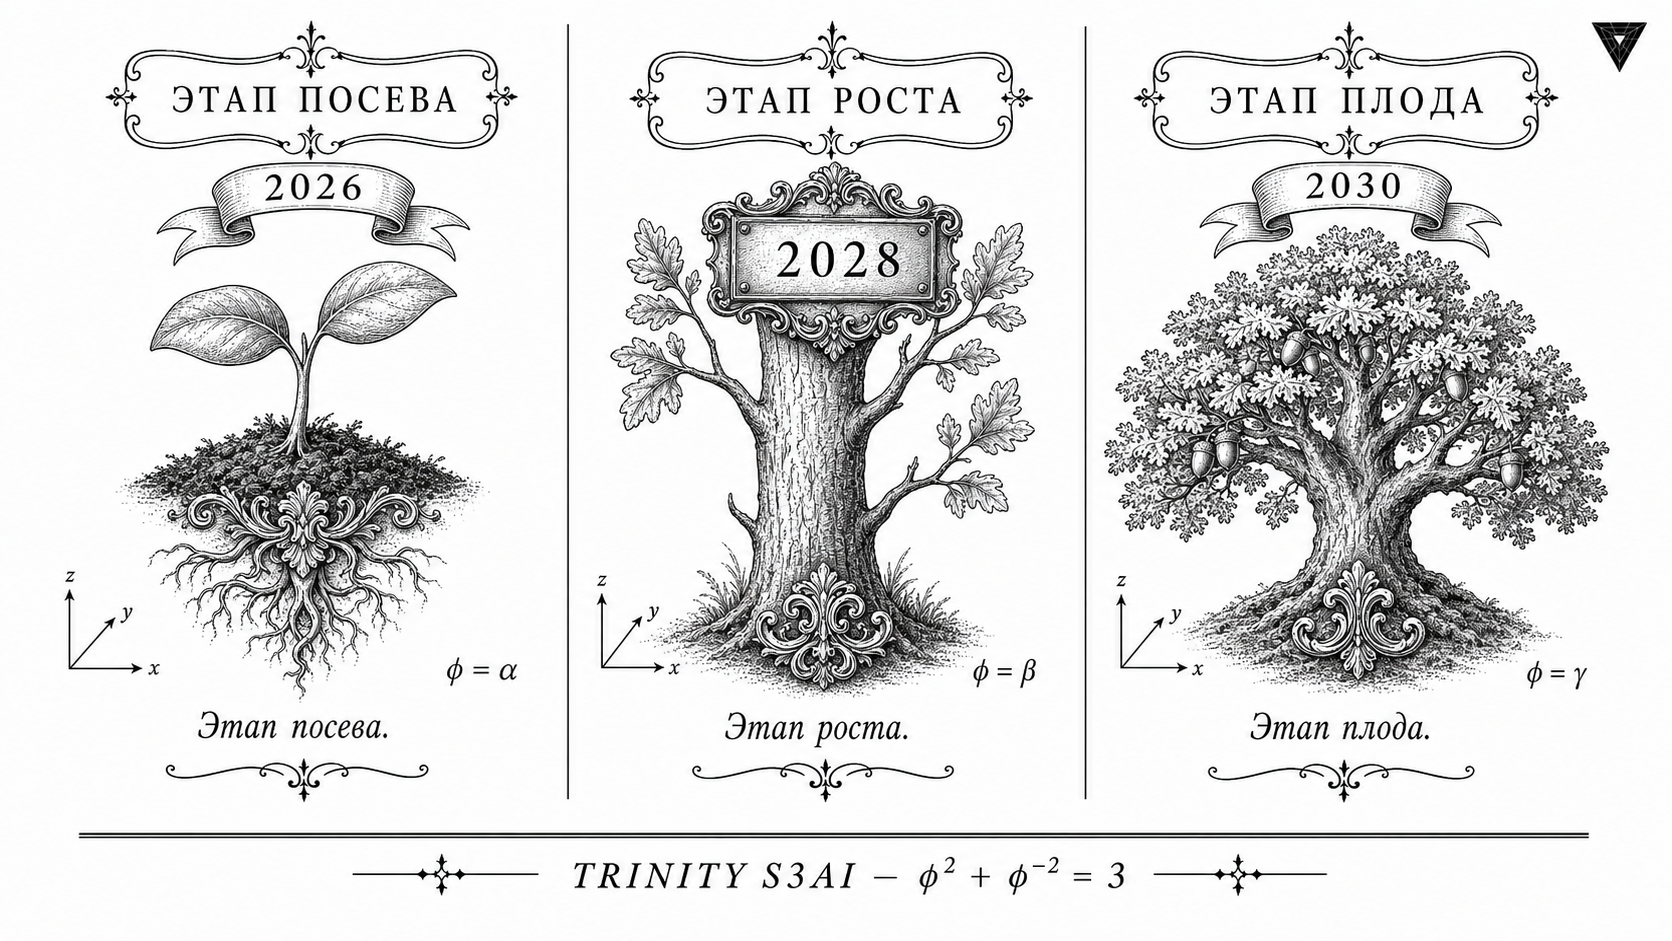
\includegraphics[keepaspectratio,alt={Триптих фиг. 8б --- Стратегия 2026--2030: посев, рост, плод.}]{figures/canon/r30_sec8b_strategy.png}}
\caption{Триптих фиг. 8б --- Стратегия 2026--2030: посев, рост, плод.}
\end{figure}

Раздел § 8a описал \emph{видение} --- глобальный контур доверия. Этот
раздел отвечает на практический вопрос: \emph{что именно делать в
2026--2030, чтобы за российским ПО закрепилась репутация доверенного ---
и внутри страны, и на экспортных рынках?} Логика стратегии ---
\textbf{национальное ядро → экспорт}: сначала собрать репутацию доверия
на действующих российских механизмах (где у государства уже есть рычаги
и нормативная база), затем спроецировать её вовне через международные
открытые стандарты прозрачности, которые понятны любому регулятору мира.

Ключевой принцип: \textbf{репутация доверия не декларируется, а
доказывается воспроизводимыми артефактами}. Не «нам можно верить», а
«вот спецификация, вот подпись, вот SBOM, вот результат сканера ---
проверьте сами». Это та же логика проверяемости, что и в тезисе «Россия
3.0» (§ 3), только применённая не к чипу, а к репутации страны как
поставщика ПО.

\subsubsection{8b.1. Два опорных контура и почему они не противоречат
друг
другу}\label{b.1.-ux434ux432ux430-ux43eux43fux43eux440ux43dux44bux445-ux43aux43eux43dux442ux443ux440ux430-ux438-ux43fux43eux447ux435ux43cux443-ux43eux43dux438-ux43dux435-ux43fux440ux43eux442ux438ux432ux43eux440ux435ux447ux430ux442-ux434ux440ux443ux433-ux434ux440ux443ux433ux443}

\textbf{Национальный контур (внутренний рынок, госзаказ, КИИ)} опирается
на действующие нормы РФ:

\begin{itemize}
\tightlist
\item
  \textbf{Реестр отечественного ПО} (ПП РФ № 1236) --- даёт приоритет в
  госзакупках; совместим с открытыми лицензиями (Apache-2.0/MIT),
  требует принадлежности прав гражданину РФ \textbf{{[}действующая
  норма{]}}
  (\href{https://meganorm.ru/Data2/1/4293758/4293758403.htm}{текст ПП РФ
  № 1236}).
\item
  \textbf{Реестр «доверенного ПО»} (ПП РФ № 1931, в силе с 01.03.2026)
  --- даёт \emph{абсолютный} приоритет в госзакупках; требует включения
  в Реестр отечественного ПО, гражданства РФ без иностранного и
  прохождения экспертизы безопасности \textbf{{[}действующая норма{]}}
  (\href{https://www.garant.ru/products/ipo/prime/doc/413066759/}{обзор
  ПП РФ № 1931, garant.ru}).
\item
  \textbf{ГОСТ Р 56939-2024 (РБПО)} ФСТЭК (с 20.12.2024) --- 25
  процессов разработки безопасного ПО (включая контроль цепочки
  поставок, SCA, работу с секретами); де-факто отраслевой чек-лист
  \textbf{{[}действующая норма{]}}
  (\href{https://docs.cntd.ru/document/1310017763/titles/6520IM}{ГОСТ Р
  56939-2024}).
\item
  \textbf{БДУ ФСТЭК} (банк данных угроз, раздел угроз ИИ 2025) и SLA по
  устранению уязвимостей (критические --- 24 ч, с 01.03.2026)
  \textbf{{[}действующая норма{]}}
  (\href{https://bdu.fstec.ru/threat/ai}{раздел угроз ИИ БДУ ФСТЭК}).
\item
  \textbf{187-ФЗ о КИИ} + Указы № 166/250 (запрет иностранного ПО на
  объектах КИИ с 01.01.2025) \textbf{{[}действующая норма{]}}.
\item
  \textbf{Ст. 1286.1 ГК РФ} --- открытые лицензии легальны в РФ;
  Apache-2.0/MIT сохраняют исключительные права правообладателя
  \textbf{{[}действующая норма{]}}
  (\href{https://rg.ru/2022/07/22/ob-ispolzovanii-svobodnyh-i-otkrytyh-licenzij-na-po.html}{о
  свободных лицензиях, rg.ru}).
\end{itemize}

\textbf{Экспортный контур (международные рынки, Глобальный Юг,
БРИКС/ШОС)} опирается на открытые стандарты прозрачности цепочки
поставок, признаваемые во всём мире:

\begin{itemize}
\tightlist
\item
  \textbf{OpenSSF Scorecard} (47 проверок, v5; сканирует 1 млн+
  OSS-проектов) --- объективная оценка зрелости безопасности репозитория
  (\href{https://openssf.org/projects/scorecard/}{OpenSSF Scorecard}).
\item
  \textbf{SLSA} (уровни L1--L3, провенанс сборки)
  (\href{https://slsa.dev}{SLSA}).
\item
  \textbf{Sigstore / cosign} (144 млн+ подписей) --- криптографическая
  подпись артефактов без управления ключами.
\item
  \textbf{SBOM} (SPDX/CycloneDX), методология \textbf{NIST SSDF SP
  800-218}, совместимость с \textbf{EU CRA} (Регламент 2024/2847, полное
  вступление 11.12.2027) и \textbf{OSV} (osv.dev, 30+ экосистем).
\end{itemize}

Эти контуры \textbf{не противоречат}: открытость стека Trinity
(Apache-2.0, открытые битовые векторы, RTL) одновременно удовлетворяет
российскому требованию «права у гражданина РФ» (лицензия сохраняет
исключительные права) и международному требованию проверяемости (любой
может воспроизвести и проверить). Один и тот же артефакт работает в
обоих контурах --- в этом стратегическая экономия.

\subsubsection{8b.2. Четыре этапа 2026--2030 с измеримыми
KPI}\label{b.2.-ux447ux435ux442ux44bux440ux435-ux44dux442ux430ux43fux430-20262030-ux441-ux438ux437ux43cux435ux440ux438ux43cux44bux43cux438-kpi}

Дорожная карта разбита на четыре годовых этапа. Каждый KPI помечен
статусом: \textbf{{[}план{]}} --- целевой ориентир стратегии (не
достигнутый результат), \textbf{{[}действующая норма{]}} --- опора на
уже принятый нормативный механизм.

\textbf{Этап 1 (2026) --- «Доказуемое ядро».} Цель: сделать каждый
репозиторий стека Trinity проверяемым по международным меркам с нулевыми
затратами.

\begin{itemize}
\tightlist
\item
  KPI 1.1: во всех публичных репозиториях --- \texttt{SECURITY.md},
  политика раскрытия уязвимостей, OpenSSF Scorecard в CI
  \textbf{{[}план{]}}.
\item
  KPI 1.2: подпись всех релизов через Sigstore/cosign; публикация SBOM
  (CycloneDX) к каждому релизу \textbf{{[}план{]}}.
\item
  KPI 1.3: подача ключевых компонентов (TRI-27, кодек GoldenFloat) в
  Реестр отечественного ПО \textbf{{[}план; опора на действующую норму
  ПП РФ № 1236{]}}.
\item
  KPI 1.4: зеркалирование репозиториев на отечественную платформу
  (GitVerse/Сбер) при сохранении публичного зеркала на GitHub
  \textbf{{[}план{]}} (\href{https://gitverse.ru}{GitVerse}).
\end{itemize}

\textbf{Этап 2 (2027) --- «Соответствие РБПО и доверенный статус».}
Цель: пройти национальные механизмы доверия и формализовать процессы
безопасной разработки.

\begin{itemize}
\tightlist
\item
  KPI 2.1: внедрение процессов ГОСТ Р 56939-2024 (РБПО) в разработку;
  самооценка по 25 процессам \textbf{{[}план; опора на действующую
  норму{]}}.
\item
  KPI 2.2: подача на включение в реестр «доверенного ПО» (ПП РФ № 1931)
  после прохождения экспертизы безопасности \textbf{{[}план; опора на
  действующую норму, в силе с 01.03.2026{]}}.
\item
  KPI 2.3: регистрация ключевых РИД (программы для ЭВМ) в Роспатенте;
  оформление лицензионной политики \textbf{{[}план{]}}.
\item
  KPI 2.4: достижение целевого балла OpenSSF Scorecard ≥ 7.0 по
  флагманским репозиториям \textbf{{[}план{]}}.
\end{itemize}

\textbf{Этап 3 (2028--2029) --- «Стандартизация и экспортная
готовность».} Цель: вписать форматы и примитивы доверия в стандарты и
подготовить экспортный пакет.

\begin{itemize}
\tightlist
\item
  KPI 3.1: участие в работе ТК 164 (ИИ) и смежных техкомитетов; вклад в
  проект ГОСТ Р «ИИ в КИИ» \textbf{{[}план{]}}
  (\href{http://tc164.ru}{ТК 164}).
\item
  KPI 3.2: согласование артефактов доверия (SBOM + SLSA-провенанс) с
  требованиями EU CRA как «обязанностей разработчика OSS-стюарда» ---
  для экспортной совместимости \textbf{{[}план; опора на Регламент EU
  2024/2847{]}}.
\item
  KPI 3.3: пилотные развёртывания с партнёрами Глобального Юга
  (БРИКС/ШОС) на FPGA --- воспроизводимый фундамент доверия без
  зависимости от закрытой литографии \textbf{{[}план{]}}.
\item
  KPI 3.4: публикация эталонных битовых векторов соответствия как
  открытого общественного актива (любая страна может проверить)
  \textbf{{[}план{]}}.
\end{itemize}

\textbf{Этап 4 (2030) --- «Россия = доверенный поставщик».} Цель:
репутация подтверждена воспроизводимыми артефактами на обоих контурах.

\begin{itemize}
\tightlist
\item
  KPI 4.1: ключевые компоненты Trinity --- в реестре «доверенного ПО» РФ
  и используются в российских проектах \textbf{{[}план{]}}.
\item
  KPI 4.2: ≥ 1 международное развёртывание/партнёрство, где российский
  стек выбран \emph{из-за} проверяемости (а не вопреки происхождению)
  \textbf{{[}план{]}}.
\item
  KPI 4.3: формат GoldenFloat и примитивы доверия признаны в ≥ 1
  международном открытом стандарте/спецификации \textbf{{[}открытая
  гипотеза/проекция{]}}.
\end{itemize}

\subsubsection{8b.3. Сводная таблица
стратегии}\label{b.3.-ux441ux432ux43eux434ux43dux430ux44f-ux442ux430ux431ux43bux438ux446ux430-ux441ux442ux440ux430ux442ux435ux433ux438ux438}

\begin{longtable}[]{@{}
  >{\raggedright\arraybackslash}p{(\linewidth - 8\tabcolsep) * \real{0.2000}}
  >{\raggedright\arraybackslash}p{(\linewidth - 8\tabcolsep) * \real{0.2000}}
  >{\raggedright\arraybackslash}p{(\linewidth - 8\tabcolsep) * \real{0.2000}}
  >{\raggedright\arraybackslash}p{(\linewidth - 8\tabcolsep) * \real{0.2000}}
  >{\raggedright\arraybackslash}p{(\linewidth - 8\tabcolsep) * \real{0.2000}}@{}}
\toprule\noalign{}
\begin{minipage}[b]{\linewidth}\raggedright
Этап
\end{minipage} & \begin{minipage}[b]{\linewidth}\raggedright
Год
\end{minipage} & \begin{minipage}[b]{\linewidth}\raggedright
Контур
\end{minipage} & \begin{minipage}[b]{\linewidth}\raggedright
Ключевой результат
\end{minipage} & \begin{minipage}[b]{\linewidth}\raggedright
Опора
\end{minipage} \\
\midrule\noalign{}
\endhead
\bottomrule\noalign{}
\endlastfoot
1 & 2026 & Экспортный + национальный & Проверяемое ядро: Scorecard,
Sigstore, SBOM, подача в Реестр ПО & ПП № 1236; OpenSSF \\
2 & 2027 & Национальный & РБПО + статус «доверенного ПО»; РИД в
Роспатенте & ГОСТ Р 56939; ПП № 1931 \\
3 & 2028--29 & Экспортный & Стандартизация (ТК 164); совместимость с EU
CRA; пилоты Юга & ТК 164; EU CRA \\
4 & 2030 & Оба & Россия = проверяемо доверенный поставщик ПО & оба
контура \\
\end{longtable}

\subsubsection{8b.4. Почему эта стратегия проходит комплайнс в обе
стороны}\label{b.4.-ux43fux43eux447ux435ux43cux443-ux44dux442ux430-ux441ux442ux440ux430ux442ux435ux433ux438ux44f-ux43fux440ux43eux445ux43eux434ux438ux442-ux43aux43eux43cux43fux43bux430ux439ux43dux441-ux432-ux43eux431ux435-ux441ux442ux43eux440ux43eux43dux44b}

Главный риск любой «национальной» стратегии доверия --- \emph{она
доверена только дома}. Стратегия Trinity снимает его архитектурно: один
и тот же открытый артефакт (спецификация + подпись + SBOM + сканер)
одновременно (а) удовлетворяет российским нормам реестра и РБПО, потому
что права принадлежат гражданину РФ и процессы формализованы, и (б)
удовлетворяет международным регуляторам (NIST SSDF, EU CRA), потому что
прозрачность цепочки поставок доказана теми же инструментами, что они
сами признают. \textbf{Доверие здесь не просят --- его дают проверить.}
Именно это делает репутацию устойчивой: её нельзя «отозвать»
политически, потому что она основана на воспроизводимых фактах, а не на
чьём-то одобрении.

Честная оговорка: всё в этом разделе с тегом \textbf{{[}план{]}} --- это
\emph{стратегические ориентиры}, а не достигнутые результаты на момент
публикации. Сегодняшний фактический задел --- опубликованные форматы и
FPGA-кодек (§ 4). Стратегия описывает реалистичный путь от этого задела
к репутации доверенного поставщика, опираясь на уже действующие нормы РФ
и уже работающие международные открытые стандарты.

\begin{center}\rule{0.5\linewidth}{0.5pt}\end{center}

\subsection{8c. Троичность за пределами кремния: классическая Trinity и
квантовые
кутриты/кудиты}\label{c.-ux442ux440ux43eux438ux447ux43dux43eux441ux442ux44c-ux437ux430-ux43fux440ux435ux434ux435ux43bux430ux43cux438-ux43aux440ux435ux43cux43dux438ux44f-ux43aux43bux430ux441ux441ux438ux447ux435ux441ux43aux430ux44f-trinity-ux438-ux43aux432ux430ux43dux442ux43eux432ux44bux435-ux43aux443ux442ux440ux438ux442ux44bux43aux443ux434ux438ux442ux44b}

\begin{figure}
\centering
\pandocbounded{
\includegraphics[keepaspectratio,alt={Триптих фиг. 10 --- Кубит → кутрит → кудит: троичность в квантовом масштабе.}]{figures/canon/r30_sec8c_qutrit.png}}
\caption{Триптих фиг. 10 --- Кубит → кутрит → кудит: троичность в
квантовом масштабе.}
\end{figure}

Здесь уместно честно очертить границу между тем, что делает Trinity, и
параллельным сюжетом квантовых вычислений, где троичность и
многозначность переживают самостоятельный подъём --- в том числе в
России.

\textbf{Что общего.} Минимальная единица Trinity --- сбалансированный
трит со значениями \(\{-1, 0, +1\}\); квантовый аналог ---
\textbf{кутрит} (трёхуровневая квантовая система) и его обобщение
\textbf{кудит} (\(d\) уровней). Один кутрит несёт
\(\log_2 3 \approx 1{,}585\) бит информации против 1 бита у двоичного
бита, что и порождает интерес к многозначным базисам и в классической, и
в квантовой инженерии. На этом уровне сбалансированная троичность ---
естественная классическая «тень» кутрита \textbf{{[}аналогия{]}}.

\textbf{Российский контекст (проверяемые факты).} Многозначные квантовые
системы --- активное направление российской науки. Группа А. К. Фёдорова
(МИСИС / РКЦ) разрабатывает алгоритмы и декомпозиции вентилей на кудитах
(\href{https://arxiv.org/html/2111.04384v3}{Nikolaeva et al., EPJ
Quantum Technology 11, 43, 2024};
\href{https://arxiv.org/html/2311.12003v2}{Kiktenko et al., Rev.~Mod.
Phys. 97, 021003, 2025}) \textbf{{[}доказано --- рецензируемые
публикации{]}}. 29 декабря 2025 г. Российский квантовый центр сообщил о
первом в России ионном квантовом компьютере на \textbf{«кусептах»} ---
7-уровневых кудитах (\(d=7\), значения \(0\!-\!6\)) на 26 ионах кальция,
эквивалентном 72 кубитам, с заявленной точностью однокудитных операций
99,92 \% и двухкудитных 96,5 \%
(\href{https://www.gazeta.ru/science/news/2025/12/29/27509077.shtml}{Газета.Ru};
\href{https://science.mail.ru/articles/42106-pervyj-v-rossii-kvantovyj-kompyuter-na-kuseptah/}{Наука
Mail.ru}) \textbf{{[}доказано --- заявление разработчика; независимая
верификация открыта{]}}. В мировой литературе троичность входит и в
квантовую коррекцию ошибок: девятикутритный код
(\href{https://arxiv.org/abs/1807.01863}{Majumdar et al.,
arXiv:1807.01863}) и GKP-кутрит за порогом безубыточности
(\href{https://www.arxiv.org/abs/2409.15065}{arXiv:2409.15065})
\textbf{{[}доказано --- публикации{]}}.

\textbf{Где проходит честная граница.} Trinity --- это
\textbf{классическая детерминированная} сбалансированная троичность:
трит имеет ровно одно из трёх значений, а вся ценность стека (§ 3, § 4a)
--- в \emph{проверяемости} (замкнутое правило вывода, битоточные векторы
соответствия, золотая эталонная модель CPU→FPGA). Кутрит/кудит
--- это \textbf{квантовая суперпозиция} трёх и более состояний; его сила
--- в амплитудах и запутанности, а не в детерминированной
воспроизводимости. \textbf{Поэтому мы прямо заявляем: Trinity --- не
квантовый чип, и никакие квантовые преимущества (ускорение,
суперпозиция, запутанность) ему не приписываются.} Любая связь между
классической троичностью Trinity и квантовыми кудитами на сегодня ---
это \textbf{аналогия и направление для будущих исследований {[}открытая
гипотеза/проекция{]}}, а не свойство существующего изделия.

\textbf{Зачем это в стратегии.} Совпадение базиса \(\{-1,0,+1\}\) с
растущим российским заделом по кудитам (РКЦ, МИСИС, ФИАН) создаёт
потенциальную точку стыковки: общий троичный «язык представления» данных
и единая открытая эталонная модель проверяемости могли бы упростить
будущие классико-квантовые мосты (например, классический трит как
естественный интерфейс к кутритному регистру). Это перспективный
исследовательский трек, а не обещание продукта \textbf{{[}открытая
гипотеза{]}}.

\begin{center}\rule{0.5\linewidth}{0.5pt}\end{center}

\subsection{9. Риски, ограничения и ответы на
контраргументы}\label{ux440ux438ux441ux43aux438-ux43eux433ux440ux430ux43dux438ux447ux435ux43dux438ux44f-ux438-ux43eux442ux432ux435ux442ux44b-ux43dux430-ux43aux43eux43dux442ux440ux430ux440ux433ux443ux43cux435ux43dux442ux44b}

\begin{figure}
\centering
\pandocbounded{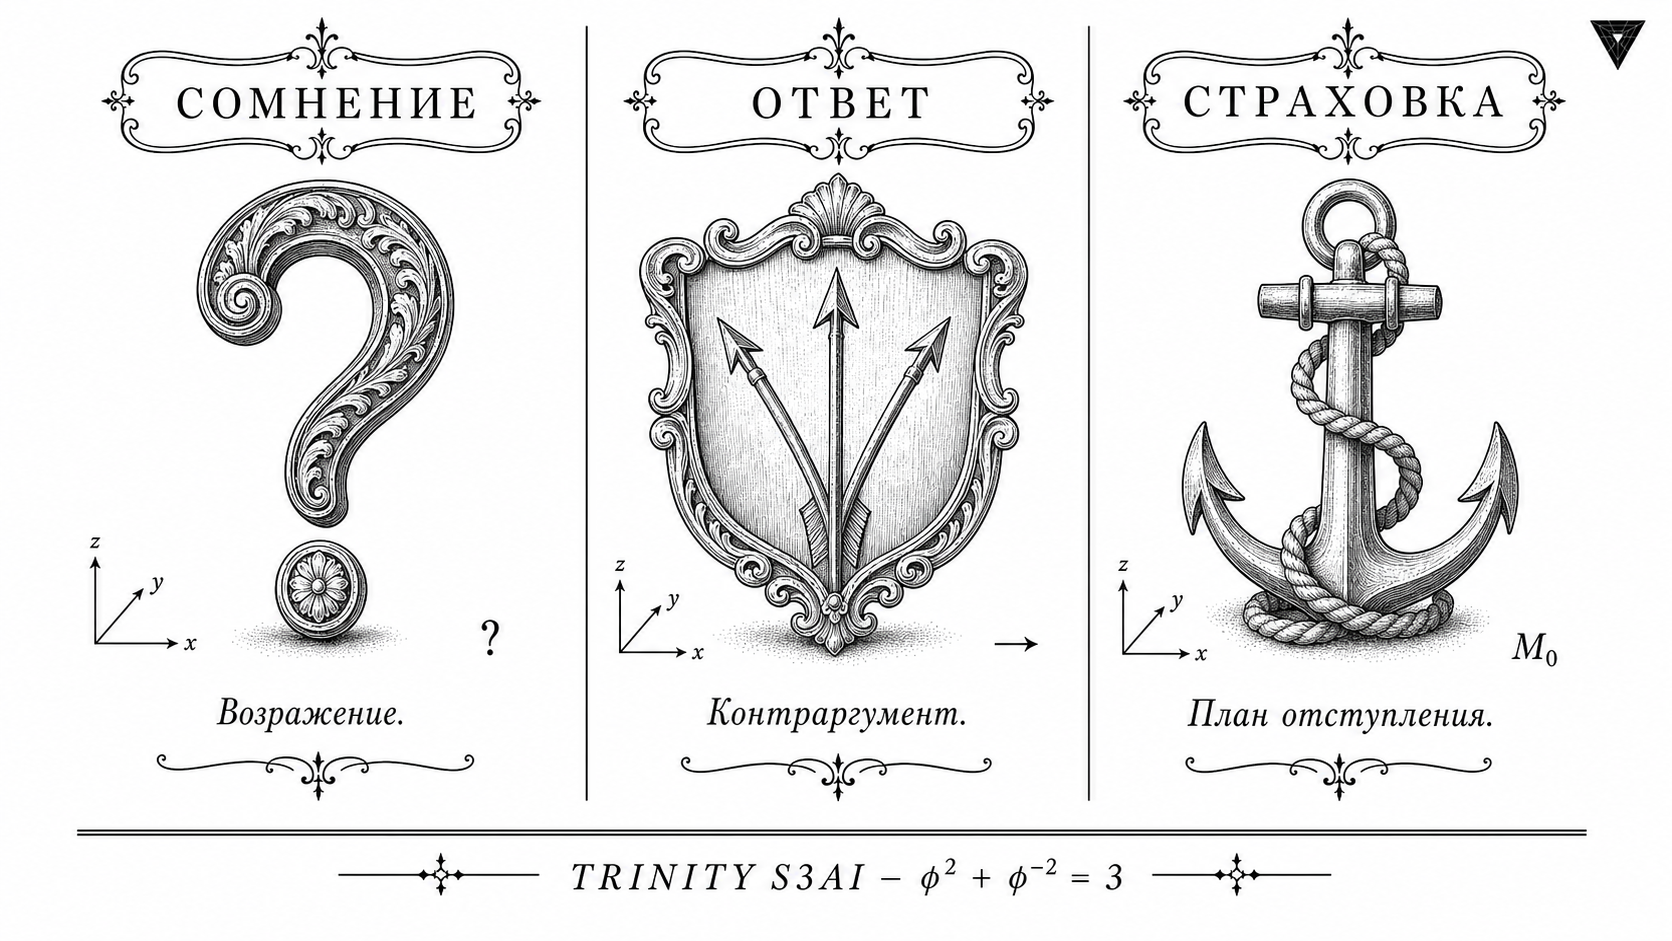
\includegraphics[keepaspectratio,alt={Триптих фиг. 9 --- Риски и контраргументы: сомнение, ответ, страховка.}]{figures/canon/r30_sec9_risks.png}}
\caption{Триптих фиг. 9 --- Риски и контраргументы: сомнение, ответ,
страховка.}
\end{figure}

Честное обращение обязано само назвать свои слабые места. Ниже ---
основные возражения и наши ответы.

\textbf{Контраргумент 1: «Зачем новый формат, если есть IEEE 754 и
posit?»} GoldenFloat не заявляет превосходства по точности (это честно
помечено как открытая гипотеза). Его ценность --- не в победе над posit,
а в \textbf{проверяемости}: замкнутое правило вывода, формальная
спецификация, битоточные векторы соответствия. Это вклад в доверенность,
а не в гонку точности \textbf{{[}открытая гипотеза по точности; доказано
по воспроизводимости{]}}.

\textbf{Контраргумент 2: «Формат никто не принял».} Верно: на июнь 2026
г. независимых цитирований и принятия вендорами нет. Это нормальный
ранний этап того же пути, по которому шёл posit. Механизм
институционализации --- не «ждать цитирований», а \textbf{стандартизация
через ПНСТ/ТК 164} и регистрация РИД \textbf{{[}открытая
гипотеза/проекция{]}}.

\textbf{Контраргумент 3: «Кремний не измерен, цифры энергоэффективности
--- проекция».} Согласны и не скрываем: изготовление кремния \textbf{не
планируется}, RTL/GDS остаются дизайн-артефактом, проверенным в симуляции и
формально; измерений на кристалле нет и не будет; любые цифры
энергоэффективности --- \textbf{{[}открытая гипотеза{]}}, оценка по
FPGA-синтезу. Проверяемый
якорь сегодня --- это \textbf{FPGA-результат GF16 (35/35 тестов, 323
МГц, плата ALINX AX7203) {[}измерено на FPGA{]}}, а не кремний.

\textbf{Контраргумент 4: «Проект держится на одном авторе» (bus
factor).} Признаём риск устойчивости. Ответ --- открытая лицензия,
контрибьюторская модель и институционализация через вуз/партнёра и
стандарт (см. § 7).

\textbf{Контраргумент 5: «Зарубежное изготовление противоречит
суверенности».} Изготовление кремния (в том числе за рубежом) \textbf{не
планируется}: текущий уровень задела --- RTL/GDS-дизайн, проверенный в
симуляции и формально, и аппаратная верификация на FPGA AX7203. Гипотетическое
будущее изготовление за рубежом сохраняло бы реальную напряжённость (см. § 5.4):
экспорт технологии (ФЗ № 183-ФЗ). Ответ --- открытые
публикуемые спецификации обеспечивают проверяемость независимо от
юрисдикции, а национальная приписка решается российским
юрлицом-лицензиатом и регистрацией РИД в РФ. Отечественное изготовление
остаётся \textbf{{[}открытой опцией/замыслом на будущее{]}}, выбор не окончателен
\textbf{{[}открытая гипотеза{]}}.

\textbf{Контраргумент 6: «``Проверяемость'' --- это маркетинг».} Именно
поэтому в § 3 она операционализирована через измеримые, фальсифицируемые
прокси (conformance vectors, воспроизводимые seals, 9/9 ширин, SSOT), а
не оставлена лозунгом.

\textbf{Контраргумент 7: «Это просьба о деньгах без отдачи».} Нет:
запрашиваемая поддержка возвращается государству неотчуждаемым
отечественным РИД (регистрируемые программа для ЭВМ и топология ИМС),
форматом-кандидатом в национальный стандарт (ПНСТ), учебной платформой и
проверяемым компонентом доверенного ИИ под действующее требование ФСТЭК
№ 117. Это инвестиция в актив, а не безвозвратная трата
\textbf{{[}доказано --- регистрируемость РИД; открытая гипотеза ---
масштаб отдачи{]}}.

\begin{center}\rule{0.5\linewidth}{0.5pt}\end{center}

\subsection{10.
Заключение}\label{ux437ux430ux43aux43bux44eux447ux435ux43dux438ux435}

\begin{figure}
\centering
\pandocbounded{
\includegraphics[keepaspectratio,alt={Триптих фиг. 11 --- Доверенная основа, троица, продолжение.}]{figures/canon/r30_sec10_conclusion.png}}
\caption{Триптих фиг. 11 --- Доверенная основа, троица, продолжение.}
\end{figure}

Рамка «Россия 3.0 --- Троица» предлагает не альтернативу государственной
стратегии, а способ её \emph{усиления}: сместить приоритет первого
порядка с производительности на проверяемость, что снимает критическую
зависимость от передовой литографии и прямо адресует самый трудный
показатель НСРИИ --- доверие граждан к ИИ. Стек Trinity S³AI приведён
как готовый отечественный пример такого подхода --- со строгим
разделением проверяемых фактов и открытых гипотез. Особо подчеркнём:
предложение опирается прежде всего на \textbf{уже действующие} нормы ---
требование доверенного ИИ в ГИС (Приказ ФСТЭК № 117), регистрируемые РИД
(ст. 1262 и 1448--1464 ГК РФ), обновлённый механизм ЭПР (258-ФЗ) --- а
не на ещё не вступивший в силу законопроект об ИИ, который привлекается
лишь как вектор регулирования. Этот метод честного фрейминга сам по себе
является вкладом: доверенность ИИ начинается с доверенности заявлений о
нём.

\begin{center}\rule{0.5\linewidth}{0.5pt}\end{center}

\subsection{Список литературы и
источников}\label{ux441ux43fux438ux441ux43eux43a-ux43bux438ux442ux435ux440ux430ux442ux443ux440ux44b-ux438-ux438ux441ux442ux43eux447ux43dux438ux43aux43eux432}

\textbf{Государственные документы:} 1. Указ Президента РФ № 490 от
10.10.2019 «О развитии искусственного интеллекта в Российской
Федерации». URL: http://www.kremlin.ru/acts/bank/44731 2. Указ
Президента РФ № 124 от 15.02.2024 (редакция НСРИИ). URL:
http://www.kremlin.ru/acts/bank/50326 3. Национальная стратегия развития
ИИ до 2030 года (актуальная редакция). URL:
https://trust-ai.ru/upload/iblock/d7f/wr0j4qwb60gkdz3n6gpe4xzs9nup6p5a.pdf
4. Нацпроект «Экономика данных и цифровая трансформация государства».
URL: https://government.ru/docs/all/138568/ 5. ГОСТ Р 59276-2020
«Системы искусственного интеллекта. Способы обеспечения доверия». URL:
https://docs.cntd.ru/document/1200177291 6. Законопроект Минцифры о
регулировании ИИ (2026, проект). URL: https://pravo.ru/news/262870/ 7.
Стратегия развития электронной промышленности РФ до 2030 (Распоряжение №
20-р от 17.01.2020). URL: http://government.ru/docs/38795/ 8. Концепция
технологического развития РФ до 2030 (Распоряжение № 1315-р от
20.05.2023). URL:
http://static.government.ru/media/files/KlJ6A00A1K5t8Aw93NfRG6P8OIbBp18F.pdf
9. Указ Президента РФ № 166 от 30.03.2022 (импортозамещение на КИИ).
URL: http://publication.pravo.gov.ru/Document/View/0001202203300001 10.
ФЗ № 258-ФЗ от 31.07.2020 «Об экспериментальных правовых режимах». URL:
http://kremlin.ru/acts/bank/45796/print 11. Перечень поручений
Президента о национальном плане ИИ (2026). URL:
https://www.cnews.ru/news/top/2026-01-06\_v\_rossii\_sozdayut\_natsionalnyj
12. Дорожная карта развития суперкомпьютеров и ИИ (март 2026). URL:
https://telesputnik.ru/materials/tech/news/mixail-misustin-utverdil-doroznuyu-kartu-razvitiya-superkompyuterov-i-texnologii-ii-v-rossii

\begin{enumerate}
\def\labelenumi{\arabic{enumi}.}
\setcounter{enumi}{12}
\tightlist
\item
  Приказ ФСТЭК России № 117 от 11.04.2025 (защита ГИС, п. 61 ---
  доверенный ИИ). URL: https://cisoclub.ru/prikaz-fstek-117/
\item
  Гражданский кодекс РФ, ст. 1262 (регистрация программы для ЭВМ). URL:
  https://www.consultant.ru/document/cons\_doc\_LAW\_5142/
\item
  Гражданский кодекс РФ, гл. 74, ст. 1448--1464 (топология ИМС). URL:
  https://base.garant.ru/10164072/
\item
  Роспатент --- регистрация топологии ИМС. URL:
  https://rospatent.gov.ru/ru/stateservices
\item
  ФЗ № 258-ФЗ об ЭПР --- закон о расширении применения (принят
  10.06.2026). URL: https://www.interfax.ru/amp/1095191
\item
  Анализ законопроекта Минцифры об ИИ (три категории моделей). URL:
  https://pravo.ru/story/263957/
\end{enumerate}

\textbf{Научно-технический задел Trinity:} 19. Vasilev D. GoldenFloat:
препринт. arXiv:2606.05017. URL: https://arxiv.org/abs/2606.05017 20.
83-форматный числовой каталог. arXiv:2606.09686. URL:
https://arxiv.org/html/2606.09686v1 21. Обзор каталога (Moonlight). URL:
https://www.themoonlight.io/en/review/an-84-format-numeric-catalog-with-bit-exact-conformance-vectors-a-vendor-neutral-reference-for-fp8-bf16-mxfp4-and-microscaling-formats
22. Репозиторий TRI-27 / t27. URL: https://github.com/gHashTag/t27

\textbf{Правовой каркас (дополнение v3):} 25. Постановление Пленума
Верховного Суда РФ № 10 от 23.04.2019 (п. 80 --- творческий вклад). URL:
https://base.garant.ru/58074501/ 26. ГК РФ, ст. 1257, 1259 (авторское
право; объект). URL:
https://base.garant.ru/5283693/abf9d030908d01fdbfee6666c1541b61/ 27.
Судебная практика по вопросам ИИ 2024--2026. URL:
https://delprof.ru/press-center/experts-pubs/sudebnaya-praktika-po-voprosam-iskusstvennogo-intellekta-2025/
28. ГК РФ, ст. 1350 (условия патентоспособности изобретения). Приказ
Минэкономразвития № 148 от 15.03.2024. URL:
https://rospatent.gov.ru/ru/news/polozhenie-o-poshlinah-2024 29.
Роспатент --- таблица патентных пошлин (льготы физлиц). URL:
https://rospatent.gov.ru/ru/activities/dues/table 30. ФЗ № 183-ФЗ «Об
экспортном контроле». URL: https://base.garant.ru/12116419/ 31. Список
товаров и технологий двойного назначения (ПП № 1299/2022, ред.). URL:
http://government.ru/docs/all/152564/ 32. Постановление Правительства РФ
№ 1931 от 28.11.2025 (доверенное ПО). URL:
http://government.ru/docs/all/162383/ 33. Постановление Правительства РФ
№ 1912 от 14.11.2023 (доверенные ПАК). URL:
http://government.ru/docs/all/150563/ 34. Постановление Правительства РФ
№ 313 от 16.04.2012 (лицензирование СКЗИ). URL:
https://base.garant.ru/70164728/ 35. Решение Коллегии ЕЭК № 30
(нотификация, Приложение 9). URL:
http://clsz.fsb.ru/files/download/reshenie\_N\_30\_prilogenie\_N\_9.pdf
35b. Gustafson J., Yonemoto I. Beating Floating Point at its Own Game:
Posit Arithmetic (2017). URL:
http://www.johngustafson.net/pdfs/BeatingFloatingPoint.pdf 35c. Hunhold
L. Beating Posits at Their Own Game: Takum Arithmetic. arXiv:2404.18603
(2024). URL: https://www.arxiv.org/abs/2404.18603 35d. Сравнение
OFP8/bfloat16/posit/takum (спектральные методы). arXiv:2504.21197. URL:
http://www.arxiv.org/abs/2504.21197 35e. BitNet b1.58 (троичные веса,
механизм сложения вместо умножения). HuggingFace blog. URL:
https://github.com/huggingface/blog/blob/main/1\_58\_llm\_extreme\_quantization.md
35f. State of Verifiable Inference (ZKP/TEE для ML). Equilibrium. URL:
https://equilibrium.co/writing/state-of-verifiable-inference 35a.
Постановление Правительства РФ № 1236 от 16.11.2015 (реестр
отечественного ПО; доля иностранного участия ≤ 49 \%), разбор требований
2026. URL:
https://terabit.ai/research/edinyj-reestr-rossijskogo-po-polnoe-rukovodstvo-po-registracii-i-meram-gospodderzhki
36. ФЗ № 162-ФЗ «О стандартизации в Российской Федерации»; ТК 164
«Искусственный интеллект». URL: https://www.garant.ru/news/1768662/

\textbf{Единая программная модель и HW/SW co-design (§ 4a):} 39.
Bachrach J. et al.~Chisel: Constructing Hardware in a Scala Embedded
Language. DAC 2012. URL: https://dl.acm.org/doi/10.1145/2228360.2228584
40. Izraelevitz A. et al.~Reusability is FIRRTL Ground: Hardware
Construction Languages, Compiler Frameworks, and Transformations. ICCAD
2017. URL: http://ieeexplore.ieee.org/document/8203780/ 41. Asanović K.
et al.~The Rocket Chip Generator. UC Berkeley Tech. Report EECS-2016-17
(2016). URL:
https://www2.eecs.berkeley.edu/Pubs/TechRpts/2016/EECS-2016-17.html 42.
AMD Vitis HLS --- высокоуровневый синтез C/C++ → RTL с C/RTL
co-simulation. URL:
https://www.amd.com/en/products/software/adaptive-socs-and-fpgas/vitis/vitis-hls.html
43. Xie et al.~PyTorch → Calyx → CIRCT (открытый HLS-маршрут).
arXiv:2512.06177 (2025). URL: https://arxiv.org/abs/2512.06177 44.
Mukherjee S. et al.~Formal Verification of a Floating-Point Unit against
a Golden C Model. arXiv:1609.00169 (2016). URL:
https://arxiv.org/abs/1609.00169 45. CREST: формальная эквивалентность
ANSI-C эталона и RTL (Oxford). arXiv:1908.01324 (2019). URL:
https://arxiv.org/abs/1908.01324 46. Armstrong A. et al.~ISA Semantics
for ARMv8-A, RISC-V, and CHERI-MIPS (Sail). POPL 2019. URL:
https://dl.acm.org/doi/10.1145/3290384 47. Ploix et al.~CHERIoT-Ibex:
доказанная эквивалентность процессора Sail-модели. arXiv:2502.04738
(2025). URL: https://arxiv.org/abs/2502.04738 48. CVA6 User Manual ---
потактовая сверка с эмулятором Spike (tandem). URL:
https://docs.openhwgroup.org/projects/cva6-user-manual/ 49. OpenTitan
Hardware Verification Methodology --- FPGA-верификация и тейп-аут из
единого RTL. URL:
https://opentitan.org/book/doc/contributing/hw/methodology.html 50.
Shanker \& Teo. Bit-Exact Python→RTL→FPGA пайплайн для INT8-квантизации
(Artix-7). Electronics 2026, 15(5), 1117. URL:
https://www.mdpi.com/2079-9292/15/5/1117 51. MPTorch-FPGA: bit-exact
обучение DNN со смешанной точностью. DATE 2025. URL:
https://ieeexplore.ieee.org/document/10993010/ 52. Shanmugavelu S. et
al.~Impacts of Floating-Point Non-Associativity (воспроизводимость FP).
arXiv:2408.05148 (2024). URL: http://arxiv.org/pdf/2408.05148.pdf 53.
Koufopoulou et al.~О границах функциональной эквивалентности HLS (≠
бит-в-бит). IEEE 2022. URL:
https://ieeexplore.ieee.org/document/9897824/ 54. Sun \& Ryoo.
Эквивалентность FPGA↔кремний и timing-corner эффекты. Electronics 2026,
15(10), 2202. URL: https://www.mdpi.com/2079-9292/15/10/2202

\textbf{Производственная и партнёрская карта (§ 3c):} 55. Список
микроэлектронных производств --- Википедия. URL:
https://ru.wikipedia.org/wiki/Список\_микроэлектронных\_производств 56.
Электронная промышленность России --- Википедия. URL:
https://ru.wikipedia.org/wiki/Электронная\_промышленность\_России 57.
Группа «Кремний ЭЛ» --- TAdviser. URL:
https://www.tadviser.ru/index.php/Компания:Группа\_Кремний\_ЭЛ 58.
Приборостроительный завод Росатома --- Википедия. URL:
https://ru.wikipedia.org/wiki/Приборостроительный\_завод\_Росатома 59.
Заводы «Интеграл», «Микрон», «Ангстрем» --- Habr. URL:
https://habr.com/ru/companies/first/articles/680224/

\textbf{Обновление 2026: конкуренты, прецеденты и бенчмарки (§ 3a.1):}
62. Yin C. et al.~TerEffic: Highly Efficient Ternary LLM Inference on
FPGA. arXiv:2502.16473 (FPL 2025). URL: https://arxiv.org/abs/2502.16473
63. Qiao Y. et al.~TeLLMe: Energy-Efficient Ternary LLM Accelerator for
Edge FPGAs. arXiv:2504.16266 (FPGA 2026). URL:
https://arxiv.org/abs/2504.16266 64. Hunhold L. Tekum: Balanced Ternary
Tapered Precision Real Arithmetic. arXiv:2512.10964 (2025). URL:
https://arxiv.org/abs/2512.10964 65. La Rosa C. L. 5500FP: 24-Trit
Balanced Ternary RISC Processor (FPGA, март 2026). URL:
https://hackaday.com/2026/03/16/ternary-risc-processor-achieves-non-binary-computing-via-fpga/
66. Wang Z. G. NANOZK: Layerwise Zero-Knowledge Proofs for Verifiable
LLM Inference. arXiv:2603.18046 (ICLR 2026 VerifAI). URL:
https://arxiv.org/abs/2603.18046 67. Wang Y. Zero-Knowledge Proof Based
Verifiable Inference (ZK-DeepSeek). arXiv:2511.19902 (2025). URL:
https://arxiv.org/abs/2511.19902 68. Peng Z. et al.~A Survey of
Zero-Knowledge Proof Based Verifiable ML. arXiv:2502.18535 (AI Review,
Springer). URL: https://arxiv.org/abs/2502.18535 69. Ploix L.-E. et
al.~CHERIoT-Ibex: Formal Verification of Observational Correctness
vs.~Sail Model. arXiv:2502.04738 (2025). URL:
https://arxiv.org/abs/2502.04738 70. Bolz-Tereick C. F. et
al.~Pydrofoil: Accelerating Sail-Based ISA Simulators. ECOOP 2025. DOI:
10.4230/LIPIcs.ECOOP.2025.3. URL:
https://doi.org/10.4230/LIPIcs.ECOOP.2025.3 71. Chung J.-W. et al.~The
ML.ENERGY Benchmark. arXiv:2505.06371 (NeurIPS 2025 Datasets \&
Benchmarks, Spotlight). URL: https://arxiv.org/abs/2505.06371 72.
Argerich M. F. et al.~Watt Counts: Energy-Aware Benchmark for
Sustainable LLM Inference. arXiv:2604.09048 (2026). URL:
https://arxiv.org/abs/2604.09048 73. Niu C. et al.~TokenPowerBench:
Benchmarking Power Consumption of LLM Inference. arXiv:2512.03024 (AAAI
2026). URL: https://arxiv.org/abs/2512.03024 74. Flocq team. coq-flocq
4.2.1 (Rocq Package, янв. 2025). URL:
https://rocq-prover.org/p/coq-flocq/4.2.1

\textbf{Обновление (июнь 2026): новая волна конкурентов и прецедентов (§
3a.2):} 75. Huang Z. et al.~TENET: An Efficient Sparsity-Aware
LUT-Centric Architecture for Ternary LLM Inference On Edge.
arXiv:2509.13765 (Microsoft Research, 2025). URL:
https://arxiv.org/abs/2509.13765 76. Guan H. et al.~TOM: A Ternary
Read-only Memory Accelerator for LLM-powered Edge Intelligence.
arXiv:2602.20662 (2026). URL: https://arxiv.org/abs/2602.20662 77. Oh H.
et al.~T-SAR: A Full-Stack Co-design for CPU-Only Ternary LLM Inference
via In-Place SIMD ALU Reorganization. arXiv:2511.13676 (DATE 2026). URL:
https://arxiv.org/abs/2511.13676 78. Dade N. O. O. et al.~Litespark
Inference on Consumer CPUs: Custom SIMD Kernels for Ternary Neural
Networks. arXiv:2605.06485 (2026). URL: https://arxiv.org/abs/2605.06485
79. Qiao Y. et al.~TeLLMe (финальная версия). ACM FPGA 2026. DOI:
10.1145/3748173.3779191. URL: https://doi.org/10.1145/3748173.3779191
80. Benno W. et al.~Jolt Atlas: Verifiable Inference via Lookup
Arguments in Zero Knowledge. arXiv:2602.17452 (2026). URL:
https://arxiv.org/abs/2602.17452 81. Liu X. et al.~Position: LLM
Inference Should Be Evaluated as Energy-to-Token Production.
arXiv:2605.11733 (2026). URL: https://arxiv.org/abs/2605.11733 82.
Deferme L. et al.~Formalizing the RISC-V Hypervisor Extension in Sail.
ACM ASPLOS 2026. DOI: 10.1145/3803525.3804982. URL:
https://doi.org/10.1145/3803525.3804982 83. Pérami T. et al.~ArchSem:
Reusable Rigorous Semantics of Relaxed Architectures. Proc. ACM Program.
Lang. (PACMPL), POPL 2026, vol.10. DOI: 10.1145/3776650. URL:
https://doi.org/10.1145/3776650 84. Wu X. et al.~QVU: A RISC-V
Vector-Extended Quantization Vector Unit for IEEE 754 and Posit Formats.
IEEE ISPA 2025. DOI: 10.1109/ISPA67752.2025.00020. URL:
https://doi.org/10.1109/ISPA67752.2025.00020 85. Li Q. et
al.~Lightweight and Precision-Scalable Posit/IEEE-754 Arithmetic in
RISC-V Cores. arXiv:2505.19096 (2025). URL:
https://arxiv.org/abs/2505.19096 86. Gül F. Energy Efficiency of AI
Hardware: A Systematic Review of GPU, TPU, and NPU Architectures in the
LLM Era. Springer, 2026. DOI: 10.1007/s44443-026-00900-6. URL:
https://doi.org/10.1007/s44443-026-00900-6 87. Cankaya B. et
al.~Bit-Exact AI Inference Verification. arXiv:2606.00279 (2026). URL:
https://arxiv.org/abs/2606.00279

\textbf{Обновление (июль 2026): ASIC-планка, AUE-метрика,
Lean/Rocq-верификация (§ 3a.3):} 88. Shan H. et al.~Platinum:
Path-Adaptable LUT-Based Accelerator for Low-Bit Weight Matrix
Multiplication. arXiv:2511.21910 (ASP-DAC 2026). DOI:
10.1109/ASP-DAC66049.2026.11420289. URL:
https://arxiv.org/abs/2511.21910 89. Zhang Y. et al.~PD-Swap:
Prefill-Decode Logic Swapping for End-to-End LLM Inference on Edge FPGAs
via Dynamic Partial Reconfiguration. arXiv:2512.11550 (2025). URL:
https://arxiv.org/abs/2512.11550 90. Zhang Y. et al.~AUE: A Normalized
Energy Efficiency Metric for AI Servers Under LLM Workloads. ICPADS
2025. DOI: 10.1109/ICPADS67057.2025.11323149. URL:
https://doi.org/10.1109/ICPADS67057.2025.11323149 91. Delavande J.,
Pierrard R., Luccioni S. Understanding Efficiency: Quantization,
Batching, and Serving Strategies in LLM Energy Use. arXiv:2601.22362
(2026). URL: https://arxiv.org/abs/2601.22362 92. Ugwuanyi E. D. et
al.~LeanBET: Formally-Verified Scientific Computing Pipeline in Lean 4.
arXiv:2605.16169 (2026). URL: https://arxiv.org/abs/2605.16169 93.
Kellison A. E. NumFuzz / Type-Based Approaches to Rounding Error
Analysis. arXiv:2501.14598 (PACMPL). URL:
https://arxiv.org/abs/2501.14598 94. Appel A., Kellison A. E. VCFloat2:
Floating-Point Error Analysis in Coq. CPP 2024. DOI:
10.1145/3636501.3636953. URL: https://doi.org/10.1145/3636501.3636953
95. Kan S., Ertel S. Interaction Tree Semantics for RISC-V: Bridging
Compiler and Hardware Verification (Rocq). arXiv:2605.04933 (2026). URL:
https://arxiv.org/abs/2605.04933 96. Maheri M. M., Haddadi H., Davidson
A. TeleSparse: Practical Privacy-Preserving Verification of Deep Neural
Networks. arXiv:2504.19274 (2025). URL: https://arxiv.org/abs/2504.19274
97. FLoPS: Semantics, Operations, and Properties of P3109 Floating-Point
Representations in Lean. arXiv:2602.15965 (2026). URL:
https://arxiv.org/abs/2602.15965 98. Advocating Energy-per-Token in LLM
Inference. arXiv:2603.20224 (2026). URL:
https://arxiv.org/abs/2603.20224 99. Geens R. et al.~Hardware Generation
and Exploration of Lookup Table-Based Accelerators for 1.58-bit LLM
Inference (KU Leuven). arXiv:2604.25183 (2026). URL:
https://arxiv.org/abs/2604.25183 100. Kourzanov P., Anmol. Modular SAIL:
dream or reality? arXiv:2507.12471 (2025). URL:
https://arxiv.org/abs/2507.12471

\textbf{Исторический контекст (троичность):} 60. Брусенцов Н. П. ЭВМ
«Сетунь» (МГУ, 1958). URL:
https://www.computer-museum.ru/articles/galglory/3226/ 61. Setun
(ternary computer). URL: https://en.wikipedia.org/wiki/Setun

\end{document}
